\documentclass[12pt,a4paper,oneside]{report}

% Page layout and typography
\usepackage[a4paper,margin=2.5cm]{geometry}
\usepackage[T1]{fontenc}
\usepackage[utf8]{inputenc}
\usepackage{lmodern}
\usepackage{microtype}
\usepackage{setspace}
\usepackage{enumitem}
\usepackage{graphicx}
\usepackage{pdflscape}
\usepackage{caption}
\onehalfspacing

\usepackage{graphicx}
\usepackage{pdflscape}
\usepackage{geometry}
\usepackage{caption}

% Mathematics
\usepackage{amsmath}
\usepackage{amssymb}
\usepackage{mathtools}

% Tables and figures
\usepackage{graphicx}
\usepackage{booktabs}
\usepackage{tabularx}
\usepackage{array}
\usepackage{float}
\usepackage{plantuml}

\usepackage{xltabular} % Recommended: handles tabularx + longtable beautifully
\usepackage{booktabs}   % For \toprule, \midrule, \bottomrule

% Quotations and citations
\usepackage{csquotes}
\usepackage[authoryear,round]{natbib}
\newcommand{\parencite}{\citep}
\renewcommand{\bibname}{References}

% The chapter uses \parencite. Add the project's bibliography as references.bib.
% Keeping this conditional allows the document to compile before that file is added.
\newif\ifbibliographyavailable
\IfFileExists{references.bib}{%
  \bibliographyavailabletrue
}{%
  \bibliographyavailablefalse
}

% Links and cross-references (load hyperref late)
\usepackage{xcolor}
\usepackage[hidelinks]{hyperref}
\usepackage[nameinlink,noabbrev]{cleveref}

% Inline code used by the methodology chapter
\newcommand{\code}[1]{\texttt{#1}}

% Prevent isolated heading lines at the foot of a page
\clubpenalty=10000
\widowpenalty=10000
\displaywidowpenalty=10000

%try
\usepackage{pdflscape}
\usepackage{tabularx}
\usepackage{booktabs}
\usepackage{array}
\usepackage{amssymb}
\usepackage{float}
\usepackage{geometry}

\newcommand{\yes}{\(\checkmark\)}
\newcommand{\partialfit}{\(\sim\)}
\newcommand{\no}{---}
\usepackage{xltabular}
\usepackage{pdflscape}
\usepackage{geometry}
\usepackage{booktabs}
\usepackage{array}
\usepackage{amssymb}
\usepackage{pdflscape}
\usepackage{tikz}

% ------------------------------------------------------------
% TeXcount configuration
% ------------------------------------------------------------

% Count words appearing inside table bodies, not only captions.
% This is needed because the university includes tables.
%TC:envir table [] otherword
%TC:envir table* [] otherword

% Count citation keys as citation occurrences rather than ignoring
% citations completely. See note below about exact citation counts.
%TC:macro \citep [text]
%TC:macro \citet [text]
%TC:macro \parencite [text]

\title{When the Decision Is Right but the Map Is Wrong: Adversarial Robustness of Identity-Document Fraud Detection and Localisation}
\author{Sush Arora}
\date{September 2026}

\begin{document}

% \pagenumbering{roman}
% \maketitle
% ============================================================
% 00_frontmatter.tex
% Front matter for the dissertation.
% Intended order: title page -> abstract -> declaration ->
% acknowledgements -> table of contents (called from main.tex).
% ============================================================

% ---- Edit these only if required ---------------------------------
\providecommand{\studentid}{U5757978}
\providecommand{\supervisorname}{Dr Muhammad Ajmal Azad}
\providecommand{\degreeprogramme}{Master of Science in Cyber Security Engineering}

% Change this filename if your existing WMG/Warwick logo uses a
% different name in the Images folder. The file still compiles if the
% image is not found, using a text fallback instead.
\providecommand{\wmglogofile}{Images/Uni_Logo.jpg}

% ------------------------------------------------------------
% Title page -- deliberately unnumbered
% ------------------------------------------------------------
\pagenumbering{gobble}
\begin{titlepage}
    \thispagestyle{empty}
    \centering

    \vspace*{0.5cm}

    \IfFileExists{\wmglogofile}{%
        \includegraphics[width=0.52\textwidth]{\wmglogofile}
    }{%
        \IfFileExists{Images/Uni_Logo.jpg}{%
            
\includegraphics[width=0.52\textwidth]{Images/Uni_Logo.jpg}
        }{%
            {\LARGE\bfseries WMG\par}
            \vspace{0.15cm}
            {\large THE UNIVERSITY OF WARWICK\par}
        }%
    }

    \vfill

    \makeatletter
    {\Large\bfseries \@title\par}
    \makeatother

    \vspace{1.4cm}
    {\large by\par}

    \vspace{1.1cm}
    \makeatletter
    {\large \@author\par}
    \makeatother

    \vspace{0.75cm}
    {\normalsize Student ID: \studentid\par}

    \vspace{1.7cm}
    {\normalsize Supervisor: \supervisorname\par}

    \vfill

    {\normalsize
    Dissertation submitted in partial fulfilment for the Degree of\par
    \vspace{0.35cm}
    \degreeprogramme\par}

    \vfill

    \begin{flushright}
        WMG\\
        University of Warwick
    \end{flushright}

    \vspace{1.2cm}

    \begin{flushleft}
        \makeatletter
        Submitted \@date
        \makeatother
    \end{flushleft}
\end{titlepage}

% ------------------------------------------------------------
% Roman-numbered front matter begins here: Abstract = i
% ------------------------------------------------------------
\clearpage
\pagenumbering{roman}
\setcounter{page}{1}

\chapter*{Abstract}
\phantomsection
% \addcontentsline{toc}{chapter}{Abstract}

% Identity-document fraud detection is a challenging field because forgery can range from small alterations like a single digit in date of birth to complex multi-faceted changes including potrait faces and identity related text fields. 
% In identity-document fraud detection, there is an increasing use of explainable artificial intelligence to detect forgery and explain the reason of the detection visually. Spatial outputs in the form of localisation maps are used for this purpose, yet a correct document-level decision does not establish that the accompanying spatial evidence identifies the manipulated region. This dissertation investigates whether an attacker with knowledge about the underlying architecture of localisation pipeline, using bounded adversarial perturbations can degrade initially acceptable spatial evidence while preserving the correct forgery decision. Such an attack can weaken trust in the use and reliability of XAI systems and potentially invalidate perfectly valid detection decisions. Two contrasting spacial output generation pipelines are evaluated on identity-document imagery: ResNet-18 with Grad-CAM as a post-hoc attribution approach, and TruFor as a native manipulation-localisation approach.

% The evaluation is organised around a novel three-stage DC--DCEC--DCEW framework. Decision Correct (DC) identifies manipulated images classified correctly before attack. Decision Correct, Evidence Correct (DCEC) retains the subset whose clean spatial maps satisfy joint relevance-mass ($E$) and relevance-rank-overlap (RRA) requirements calibrated from clean development evidence and visual review. Decision Correct, Evidence Wrong (DCEW) then records attacks that preserve the correct decision while causing either evidence requirement to fail. 
% The study also conducts additional Clean-data audits to examine possible shortcut cues and regional sensitivity, while classification-targeted attacks provide complementary controls. Each pipeline is assessed against its own clean baseline, with uncertainty estimated through document-stem resampling and shared eligible images used as an additional comparison view.

% The study provides a comprehensive analysis of benchmark dataset in ID fraud detection 'FantasyID' dataset and its limitations, identifies the need for newer metrics which can assit in the complex task of ID forgery detection, proposes novel framework of DC-DCEC-DCEW for robustness of detection and localisation pipelines and also highlikghts the need for further creation of datasets which can be used for research purposes and that model the real word scenario's. 

% The study therefore evaluates a distinct reliability risk: spatial forensic evidence can require separate robustness assessment even when the associated forgery decision remains correct. The conclusions are bounded by the selected dataset, model pipelines, spatial criteria and attack configurations, and do not constitute evidence of a verification bypass or of human-review performance.
\addcontentsline{toc}{chapter}{Abstract}

Identity-document fraud detection is challenging because manipulations can range from small textual changes, such as a single digit in a date of birth, to complex multi-region alterations involving portraits and identity-related text fields. Spatial outputs are used alongside forgery decisions to indicate where manipulation may have occurred. However, a correct document-level decision does not establish that the accompanying spatial evidence identifies the manipulated region. This dissertation investigates whether, under a white-box threat model, bounded adversarial perturbations can degrade initially acceptable spatial evidence while preserving the correct forgery decision. Such an attack can undermine trust in the spatial evidence accompanying an otherwise correct forgery decision. Two contrasting spatial-output pipelines are evaluated on identity-document imagery: ResNet-18 with Grad-CAM as a post-hoc attribution approach, and TruFor as a native manipulation-localisation approach.

The evaluation is organised around a three-stage DC--DCEC--DCEW framework. Decision Correct (DC) identifies manipulated images classified correctly before attack. Decision Correct, Evidence Correct (DCEC) retains the subset whose clean spatial maps satisfy joint relevance mass accuracy ($E$) and relevance rank accuracy (RRA) requirements, with thresholds calibrated using clean development evidence and visual review. Decision Correct, Evidence Wrong (DCEW) then records attacks that preserve the correct decision while causing either evidence requirement to fail. The study also conducts clean-data audits to examine possible shortcut cues and regional sensitivity, while classification-targeted attacks provide complementary controls. Each pipeline is assessed against its own clean baseline, with uncertainty estimated through document-stem resampling and shared eligible images used as an additional comparison view.

The study provides a detailed analysis of the FantasyID dataset and its limitations, demonstrates the value of complementary mass- and rank-based measures for assessing spatial evidence, and proposes the DC--DCEC--DCEW framework for evaluating the robustness of detection and localisation pipelines. It also highlights the need for future datasets that better represent the diversity and complexity of real-world identity-document fraud scenarios.

The study therefore evaluates a distinct reliability risk: spatial forensic evidence can require separate robustness assessment even when the associated forgery decision remains correct. The conclusions are bounded by the selected dataset, model pipelines, spatial criteria and attack configurations, and do not constitute evidence of a verification bypass or of human-review performance.
\clearpage
\chapter*{Declaration}
\phantomsection
\addcontentsline{toc}{chapter}{Declaration}

I have read and understood the University rules concerning academic integrity, plagiarism and appropriate referencing. I declare that the work presented in this dissertation is my own except where the contribution of others has been clearly acknowledged and referenced.

No substantial part of this dissertation has been submitted by me for assessment on another course or degree, except where this has been explicitly declared in accordance with University requirements.

% If WMG provides mandatory declaration wording for your programme,
% replace the two paragraphs above with the current official wording.

\clearpage
\chapter*{Acknowledgements}
\phantomsection
\addcontentsline{toc}{chapter}{Acknowledgements}

I would like to thank my parents and my life partner for their patience, encouragement and constant support throughout my studies. I am grateful to my supervisor, \supervisorname, and to the WMG teaching team for their guidance and feedback during the programme and this dissertation.

I also thank my in-laws for their support, and my university friends, with whom the long hours, shared challenges and hard work have created new and valued friendships.

\tableofcontents
\clearpage

\pagenumbering{arabic}


% Chapter 1, version 7 (01V7.tex): 21 September 2026.
% Supersedes the supplied 01V6.tex; existing section/objective labels retained.
% V7: bold problem statement, explained/repositioned risk figure, agreed RQ scope.
% Uses the citation keys already present in the supplied Chapter 1.
% Risk diagram: Images/CH01_02_revised.pdf, with Images/CH01_02.png as fallback.
% The risk diagram is fixed after the Section 1.2 explanation (requires float).
% Optional new figure: Images/CH01_DCEC_DCEW.pdf (prompt supplied separately).
% Threshold values and unfinished experiments are deliberately not asserted.

\chapter{Introduction}

\label{ch:introduction}

\section{From physical to image-based verification}
\label{sec:intro-document-as-image}

Modern identity documents have a long history, including medieval safe-conducts protected by the English Safe Conducts Act 1414 \citep{McHugh2021,SafeConducts1414}. Their value as evidence nevertheless depends on establishing that the document is genuine and belongs to the person presenting it.

The digital-first economy has changed how these documents are checked. Consumers now open bank accounts remotely, and the physical ID may be flattened into a smartphone photograph and examined through software. Remote services can inspect visible security features or incorporate chip reading, but a single photograph cannot provide the same evidence as handling a document or accessing its electronically stored information \parencite{GovUK2018}. NIST's guidelines recognise remote unattended proofing, where automated checks do not require interaction with a proofing agent \citep{nist2025sp80063a}.

This workflow creates different opportunities for cyber criminals. Where an attacker can submit or inject a modified image, the forgery can target the captured pixels without requiring a convincing physical counterfeit. International security and law-enforcement agencies recognise identity and document fraud as facilitating wider criminal activity \parencite{EuropolSOCTA2025, frontex2025ara}. Driven by this changing threat landscape, researchers therefore evaluate both manipulation detection and spatial localisation \citep{LuoICDAR2023,GuanOpenMFC2022} through shared datasets and benchmark competitions organised by bodies such as IAPR and NIST. The first asks whether a document was altered; the second asks where.

Spatial outputs also appear in commercial services. IDVerse reports using a neural network for document authentication, while Shufti provides heatmaps highlighting suspected alterations \citep{LexisNexis2025IDVerse,Shufti2025Heatmaps}. Such maps can support inspection, but neither commercial adoption nor greater spatial detail establishes their correctness.


\section{From performance to dependable evidence}
\label{sec:intro-performance-to-evidence}

\begin{samepage}
\hrule
\vspace{0.6em}
\noindent\textbf{\underline{Problem addressed:}} A correct forgery decision does not establish that the accompanying spatial map identifies the altered region. This thesis investigates whether bounded adversarial perturbations can degrade initially acceptable spatial evidence while preserving that correct decision.\par
 \vspace{0.9em}
\hrule
\end{samepage}
\vspace{0.8em}
Neural forensic detectors learn patterns in image acquisition, editing and compression \parencite{verdoliva2020overview}. TruFor, for example, combines noise-sensitive features with RGB information to produce a spatial anomaly map and a document-level score \parencite{guillaro2023trufor}. These outputs answer different questions and require separate evaluation.

Learned detectors may also exploit dataset-specific shortcuts. Compression or capture-device differences can separate training classes without representing the manipulation itself \parencite{geirhos2020shortcut,Lapuschkin2019CleverHans}. Processing inconsistencies can provide useful forensic evidence, but they may also reflect how the dataset was assembled. The clean-data audit examines this distinction before adversarial degradation is interpreted.

Adversarial perturbations are deliberately optimised pixel modifications that target model behaviour within a specified budget \parencite{goodfellow2015explaining,szegedy2014intriguing}. It is important to consider that a document may already contain a swapped portrait or altered text before a subsequent perturbation is applied. Throughout this study, \emph{clean} means before this additional perturbation; a clean image can therefore already contain a forgery. The concern is that a reviewer receives the correct warning with forgery detection but a less useful indication of where the alteration lies from spatial maps.

Figure~\ref{fig:risk-summary-critical} follows these routes from the document to the detector's outputs. The left-hand branch shows how dataset shortcuts can undermine decisions or spatial evidence before an attack. The right-hand branch separates attacks, that change the decision from those that degrade spatial evidence while preserving it. The highlighted route with double red boxes is the focus of this thesis. The other routes explain the need for clean-data checks and classification-attack controls.

% Fixed here so the diagram follows its explanation and precedes Section 1.3.
\begin{figure}[H]
\centering
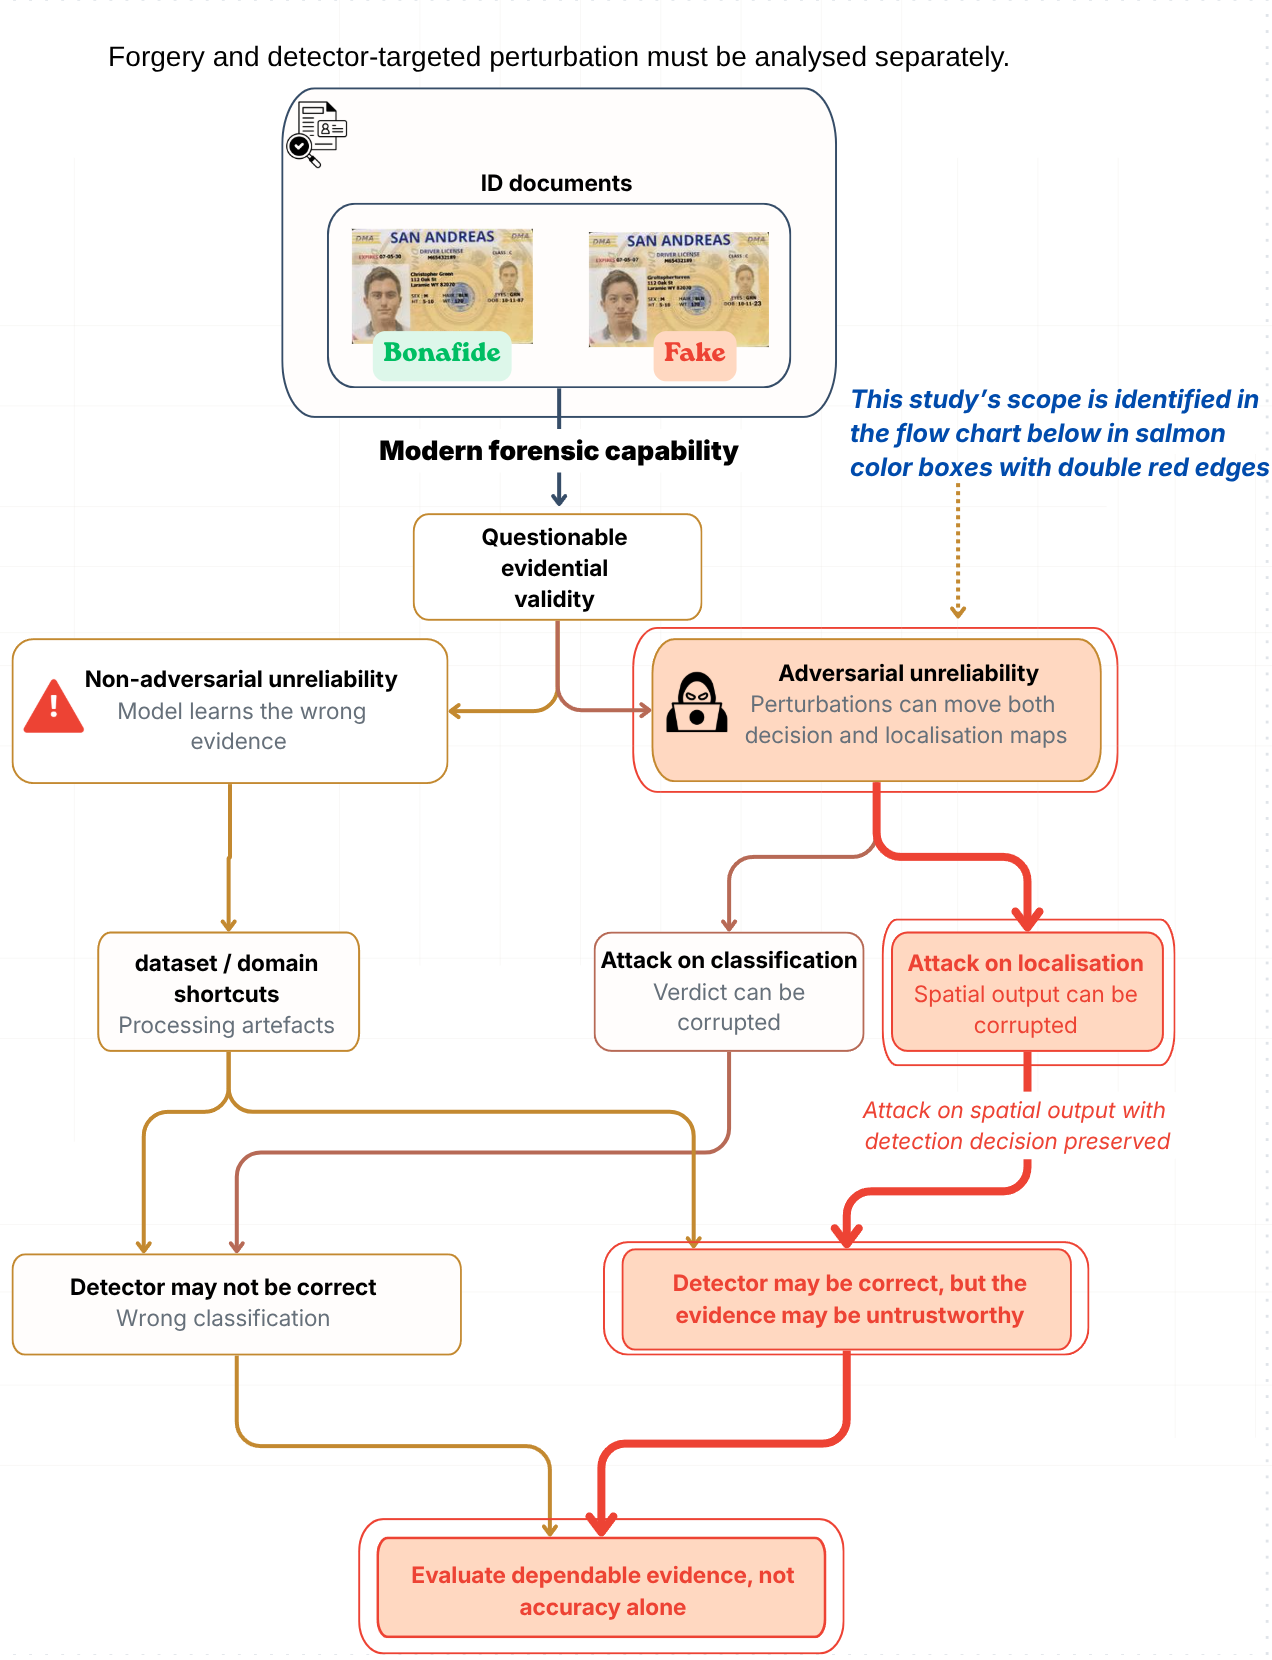
\includegraphics[width=0.95\textwidth,height=0.73\textheight,keepaspectratio]{Images/CH01_02.png}
\caption{Conceptual routes to unreliable forensic outputs. Arrows show possible routes to failure; the highlighted route with double red boxes concerns degradation of spatial evidence while the correct forgery decision is preserved.}
\label{fig:risk-summary-critical}
\end{figure}
%------------------------------------------------------------------
\clearpage
\section{Two ways of producing spatial evidence, and what is not known}
\label{sec:intro-two-paradigms-gap}

Learned detectors produce spatial evidence in two different ways.

\begin{enumerate}
    \item \textbf{Post-hoc attribution:} A classifier returns a score, and an attribution method such as Grad-CAM is applied afterwards to indicate regions contributing to the target score \parencite{Selvaraju2017GradCAM}. The map is an inference about the classifier, rather than an output it was trained to produce.
    \item \textbf{Native manipulation-localisation:} A purpose-built system such as TruFor is trained to estimate manipulated regions directly. Its spatial map is a supervised prediction, accompanied by confidence and detection outputs \parencite{guillaro2023trufor}.
\end{enumerate}

These outputs have different meanings. Agreement with manipulation annotations asks whether a map identifies the labelled regions. Explanation faithfulness asks whether it reflects the classifier's behaviour. This study concerns the first property and its vulnerability to attack; spatial agreement alone does not establish the second.

Earlier work demonstrates prediction-preserving attacks on explanations and attacks on forensic localisers \parencite{ghorbani2019fragile,dombrowski2019explanations,cao2024transferable}. The studies reviewed in Chapter~2 do not establish how initially acceptable spatial evidence degrades under a decision-preserving constraint in both kinds of pipeline on identity-document images.

FantasyID supplies complete document images, physical print-and-capture conditions, manipulated face and text regions, and public annotations \parencite{korshunov2025fantasyid}. ResNet-18 with Grad-CAM and TruFor represent the two routes. Each pipeline is evaluated against its own clean performance. The aim is to measure vulnerability within that performance, rather than to develop a higher-scoring detector.

The analysis follows three stages:
\begin{enumerate}
    \item \textbf{DC(Decision Correct):} Identify manipulated images correctly classified before adversarial perturbation.
    \item \textbf{DCEC(Decision Correct, Evidence Correct):} Within DC, retain images whose clean maps meet both a relevance-mass requirement and a relevance-rank-overlap requirement against the annotations.
    \item \textbf{DCEW(Decision Correct, Evidence Wrong):} Within the fixed clean DCEC set, count attacks that preserve the correct decision but cause either evidence requirement to fail.
\end{enumerate}

Relevance mass accuracy ($E$) measures how much map mass lies inside the annotation. Relevance rank accuracy (RRA) measures how far a set of the strongest map pixels, equal in size to the annotated region, overlaps it. ``Evidence correct'' therefore means passing this study's spatial criterion. The protocol requires thresholds to be calibrated using clean development evidence and fixed before evaluating DCEC-to-DCEW outcomes. Both pipelines follow the same calibration procedure, although their numerical thresholds may differ. Within each pipeline, the same thresholds apply to clean and adversarial maps.

Reporting the numbers reaching DC and DCEC keeps limited coverage visible. Classification flips remain in the DCEC denominator and are reported separately. Images qualifying for both pipelines provide an additional view of each pipeline's degradation; they do not remove differences in architecture, training or map resolution.

% This figure is included automatically once the prompted artwork is added.
\IfFileExists{Images/CH01_DCEC_DCEW.pdf}{%
Figure~\ref{fig:dc-dcec-dcew} summarises the analysis populations and outcomes.
\begin{figure}[tbp]
\centering
\includegraphics[width=\textwidth,height=0.66\textheight,keepaspectratio]{Images/CH01_DCEC_DCEW.pdf}
\caption{DC, DCEC and adversarial outcomes. Clean eligibility fixes the denominator. An evidence failure counts as DCEW only while the decision remains correct.}
\label{fig:dc-dcec-dcew}
\end{figure}
}{}

\section{Aim, research question and objectives}
\label{sec:intro-aim-rq-objectives}

This dissertation evaluates whether bounded adversarial perturbations can undermine initially acceptable spatial evidence while preserving a correct identity-document forgery decision.

\begin{quote}
\noindent\textbf{Research question.} To what extent can bounded adversarial perturbations degrade initially acceptable spatial evidence from post-hoc attribution and native localisation while preserving the correct identity-document forgery decision?
\end{quote}

This question is investigated using ResNet-18 with Grad-CAM and TruFor. Each pipeline is evaluated against its own clean performance. Chapter~2 explains the reasons for selecting these models.

The following five objectives address this question.

\crefname{enumi}{objective}{objectives}
\Crefname{enumi}{Objective}{Objectives}
\begingroup
\renewcommand{\theenumi}{O\arabic{enumi}}
\renewcommand{\labelenumi}{\textbf{\theenumi.}}
\begin{enumerate}
    \item\label{obj:baselines} Establish clean detection and spatial-agreement baselines under documented preprocessing, reporting the images and forgery families each pipeline can support.
    \item\label{obj:evidence} Audit compression-related cues and regional sensitivity, and calibrate the joint $E$ and RRA criterion using clean-development measurements and a visual review conducted without access to those measurements.
    \item\label{obj:attack} Evaluate bounded, white-box attacks on spatial evidence, measuring DCEC-to-DCEW transitions and continuous degradation while reporting decision preservation. Use classification-targeted attacks as complementary controls.
    \item\label{obj:compare} Assess each pipeline against its own clean baseline, quantify uncertainty using document-stem resampling, and examine shared eligible images and visual examples as an additional analytical view.
    \item\label{obj:implications} Synthesise the findings to identify when spatial outputs support manipulation assessment, explaining the practical value, remaining risks and limits of the evidence.
\end{enumerate}
\endgroup

\section{Contribution}
\label{sec:intro-contribution}

The contribution is an evaluation of attacks that undermine spatial evidence while preserving correct forgery decisions. Its outputs are clean coverage estimates, conditional DCEC-to-DCEW rates and continuous changes in spatial agreement. The clean audit supplies the context needed to distinguish an attack-induced failure from evidence that was already inadequate.

For financial-services practitioners, the study examines whether a map accompanying a correct forgery warning can become less useful for inspecting the document. It does not demonstrate a verification bypass or measure how human reviewers respond. For researchers, it provides a documented evaluation framework and experimental evidence for studying this failure.

The claims remain bounded by the selected dataset, pipelines and attack configurations. Rectangular annotations approximate manipulated regions, and the maps differ in meaning and resolution. These limits remain relevant when interpreting degradation relative to each pipeline's clean baseline.

\section{Structure of the dissertation}
\label{sec:intro-structure}

Chapter~2 reviews the datasets, spatial outputs, evaluation measures and adversarial literature. Chapter~3 defines the methodology, calibration and risk controls. Chapter~4 reports clean performance and DCEC coverage; Chapter~5 evaluates adversarial degradation. Chapter~6 discusses the findings and concludes. Supporting detail is organised in Appendix~A for metric calibration and sensitivity checks, Appendices~B and~C for ResNet-18 and TruFor decisions and risk registers, and Appendix~D for reproducibility records.

% Chapter 2, version 1 (02V1.tex): 21 September 2026.
% Supersedes the supplied 02V0(1).tex. Existing active section labels retained once.
% Required packages: amsmath, graphicx, booktabs, array, tabularx, natbib.
% Figure: Images/CH02_MassRank_V1.pdf (supplied with this revision).
% References: merge Chapter_02_References_V1.bib by citation key; do not duplicate keys.
% Calibration thresholds and incomplete experiments are not presented as completed.

\chapter{Literature Review}
\label{ch:litreview}

% \section{Introduction}
% \label{sec:lr-intro}

% A forgery detector neural network pipeline can make the correct decision between bona-fide and forged identification document(ID) while giving a poor indication on the spatial map, as to where the alteration lies. This chapter reviews the literature needed to investigate whether an adversary can create that failure from an initially useful spatial map. This included research into identity-document datasets, spatial map generation techniques including post-hoc attribution and native localisation, and attacks on spatial outputs. It then explains the choice of relevance mass and rank accuracy, and how these established metrics and measures support this study's DC--DCEC--DCEW framework.

% The review connects findings to the research choices they support. Dataset and pipeline selection inform the clean baselines in O1; limitations of spatial measures inform the audit and calibration in O2; adversarial studies inform O3 and O4. Its scope is a focused critical review of these connected areas. The research gap concerns a particular conditional failure, rather than a claim that spatial maps have not previously been attacked.

\section{Introduction} \label{sec:lr-intro} A forgery detector neural network pipeline can make the correct decision between bona-fide and forged identity document (ID) while giving a poor indication on the spatial map, as to where the alteration lies. This distinction is particularly important because IDs have many semantically distinct regions such as portraits, biographical text and document identifiers, coexisting with graphical and security features that are issuing authority specific. ID forgery may affect anything from a small part of a textual field to an entire portrait. 

Before considering attacks on spatial evidence, it is therefore necessary to establish the characteristics of ID forgery as a forensic problem. This chapter reviews the literature needed to investigate whether an adversary can degrade an initially useful spatial map while preserving the detector's forgery decision. It considers the domain-specific characteristics of manipulated IDs and the datasets available for studying them. 

It then reviews two routes to spatial evidence followed by methods for evaluating spatial agreement and adversarial work targeting spatial outputs. These strands motivate the use of relevance mass and relevance rank accuracy and support this study's DC--DCEC--DCEW framework. 

The review connects findings to the research choices they support. 
\begin{enumerate}[itemsep=1pt]
    \item Dataset and pipeline selection inform the clean baselines in O1
    \item Limitations of spatial measures inform the audit and calibration in O2
    \item Adversarial studies inform O3 and O4.
\end{enumerate}

Its scope is therefore a focused critical review of the literature needed to examine whether spatial evidence that is acceptable on a correctly detected forged ID can be degraded without changing the forgery decision. The research gap is this domain-specific conditional failure evaluation rather than a claim that spatial maps have not previously been attacked.

% \section{Manipulated identity document as a forensic problem}
% \label{sec:lr-context}

% In remote verification, software often examines a photograph of a document. A digitally replaced portrait or an edited date of birth can therefore reach a detector without the attacker producing a convincing physical counterfeit. FantasyID models this digital-manipulation setting using face swapping and text inpainting \citep{korshunov2025fantasyid}. The later adversarial perturbation studied here is a separate change to that already manipulated image.

% Hence in the remote verification, two naturally arising questions are:
% \begin{enumerate}
%     \item Whether the document is forged
%     \item Whether detectors pipeline's spatial output directs attention towards the alteration.
% \end{enumerate}

% Neither answer establishes how a person using remote verification pipeline in banking or law enforcement agencies will use the map. NIST's Explainable AI principles distinguishes an explanation that is user-centric and understandable from an explanation that embeds model fidelity and accurately reflects the system's process \citep{phillips2021four}. This distinction motivates careful evaluation, but annotation agreement alone cannot demonstrate explanation faithfulness or improved human in the loop's decisions. The present study evaluates spatial agreement. It does not test a banking verification service or its reviewers.

%--------------------------------------------------------------------------------------------------
\section{Identity-document forgery as a domain-specific forensic problem} \label{sec:lr-context} 

International specifications for machine-readable travel documents define standards for physical dimensions, visual data layouts, and machine-readable zones to ensure global interoperability. The framework also addresses guidelines for protecting biographical data against alteration and establishes electronic chip and cryptographic standards \citep{icao9303}. For certification of remote verification software, FIDO's standardised test criteria include features such as holograms, guilloché patterns, microprinting, ghost images, specialised fonts, and interactions between the primary portrait and the document background \citep{fido2026docauth}. 

Consequently, IDs are a structured security artefact but not all of the physical security properties are observable from a single digital photograph used in remote verification. Some features depend on illumination, viewing angle, wavelength or electronic access. Since remote verification commonly operates on captured or uploaded document images, it makes it possible for alterations to the visually observable identity fields to reach an automated detector without the attacker constructing a complete physical counterfeit. The forensic problem considered in this thesis is restricted to this digital-image setting. 

Within that setting, the spatial scale and semantic importance of a manipulation can vary substantially. Altering one or more characters in a date of birth, name or document number may modify only a very small image region while materially changing the represented identity. At the other extreme, a portrait may be partially modified or replaced entirely. The DeepID challenge identifies this combination of high-value targets including names, dates, identification numbers and facial portraits as a distinctive difficulty in ID manipulation detection, and treats document-level detection and pixel-level localisation as separate forensic tasks \citep{korshunov2025deepid}. FantasyID models the same digital-manipulation setting using face-swapping and text-inpainting attacks and provides annotations of the manipulated regions \citep{korshunov2025fantasyid}. 

These properties also affect the learning formulation. A generic whole-image representation need not explicitly encode that a small change inside a date field can have greater forensic significance than a visually larger change in an irrelevant background region. Recent field-localised work therefore argues for explicitly modelling semantically important regions such as portraits and textual fields rather than treating the entire document as homogeneous image content \citep{kumar2026flid}. 

By explicitly representing manipulation classes during training, supervised modelling enables the system to learn the domain structure directly from the available labels. This does not mean that unsupervised or self-supervised approaches are unsuitable for ID fraud. A purely closed-set supervised detector may fail to represent new document layouts, fabrication processes or previously unseen fraud strategies. Recent work on open-set ID-fraud discovery consequently combines document-specific representation learning with self-supervised and supervised objectives to identify anomalous and previously unseen fraud patterns \citep{li2026layoutaware}. Supervised detection and open-set anomaly discovery should therefore be viewed as complementary responses to different parts of the problem. 

The present study concerns known digital manipulation families for which labels and alteration regions are available, making supervised detection and explicit spatial evaluation appropriate to the research question. 

In remote verification pipelines, two naturally arising questions are: 
\begin{enumerate} [itemsep=1pt]
\item Does the pipeline correctly classify the document as forged? 
\item Does its spatial output direct evidence towards the known alteration? 
\end{enumerate} 

A correct answer to the first question does not imply a useful answer to the second. A detector may exploit document-wide acquisition or processing traces, or other predictive cues outside the altered field, and still produce the correct document-level decision. 

This separation between decision correctness and spatial agreement motivates the clean evidence conditions introduced later in this chapter. The adversarial perturbation studied in this thesis is a further, separate modification applied to an already forged image. Its purpose is not to create the underlying identity-document forgery, but to test whether initially acceptable spatial evidence can be degraded while the forgery decision is preserved.
%--------------------------------------------------------------------------------------------------
% \section{Datasets and the selection of FantasyID}
% \label{sec:lr-data}

% The dataset must provide complete document images and known manipulation regions. Capture conditions also matter because a forensic model may use processing traces that disappear in digitally rendered images. Table~\ref{tab:lr-datasets} compares the main alternatives against these requirements.

% \begin{table}[htbp]
% \centering
% \small
% \renewcommand{\arraystretch}{1.15}
% \caption{Dataset suitability for whole-document spatial evaluation. Limitations refer to the needs of this study.}
% \label{tab:lr-datasets}
% \begin{tabularx}{\textwidth}{@{}>{\raggedright\arraybackslash}p{0.23\textwidth}>{\raggedright\arraybackslash}X>{\raggedright\arraybackslash}X@{}}
% \toprule
% Dataset & Useful evidence & Main limitation here \\
% \midrule
% MIDV-2020 \citep{bulatov2022midv2020} & Mock documents across photographs, scans and videos. & Recognition benchmark without paired digital-forgery masks. \\
% SIDTD \citep{boned2024sidtd} & Extends mock documents with crop-and-replace and inpainting attacks. & Constructed templates and attack generation differ from the selected setting. \\
% IDNet \citep{guan2024idnet} & Large synthetic collection with varied document types and fraud patterns. & Digital renders do not reproduce the same physical capture history. \\
% FakeIDet2 / FakeIDet3-DB \citep{munozharo2026fakeidet2,munozharo2026fakeidet3} & Privacy-aware patches from real IDs; the newer release adds digital attacks. & Released patches do not preserve complete-document spatial context. \\
% FantasyID \citep{korshunov2025fantasyid} & Complete captured cards, face/text edits and region annotations. & Fictional layouts, approximate masks and repeated captures limit generalisation. \\
% \bottomrule
% \end{tabularx}
% \end{table}

% These alternatives address different problems. MIDV-2020 supports recognition under capture variation, while SIDTD adds forgery examples. IDNet prioritises scale through synthesis. FakeIDet2 brings real-document traces into a privacy-aware benchmark; FakeIDet3-DB extends this approach to classical and generative digital attacks. The large IDNet release and FakeIDet3-DB are described in preprints, so their reported capabilities warrant the same scrutiny as their useful data contributions.

% FantasyID offers the closest fit among these datasets: physical print-and-capture, complete images, portrait and text manipulations, and annotations. Its original study also reports substantial test errors at a validation-selected operating point, despite useful ranking performance \citep{korshunov2025fantasyid}. Thus, published detection performance does not establish that enough individual images have useful spatial evidence for an adversarial study. Clean eligibility must be measured directly.

% The DeepID challenge provides further identity-document evidence, including TruFor baselines and submissions evaluated on a private real-document set \citep{korshunov2025deepid}. That private evaluation cannot be reproduced from FantasyID alone. The challenge report also records a team's observation of different JPEG quality factors for bona-fide and manipulated images. This motivates a compression audit, rather than assuming that a correct decision necessarily reflects the edited field. Shortcut learning offers the broader explanation: models can exploit predictive features that fail outside the training setting \citep{geirhos2020shortcut}.

% Three limitations remain after dataset selection. Rectangular annotations approximate the altered regions; capture variants of one card are dependent observations; and fictional documents cannot establish performance across real issuing authorities. These motivate mask-sensitivity checks, grouping by document stem and restricted claims. Chapter~3 defines these controls; Appendix~A records metric-related risks and the model-specific registers retain preprocessing decisions.

%--------------------------------------------------------------------------------------------------

\section{Datasets, assurance criteria and the selection of FantasyID}
\label{sec:lr-data}

Dataset selection is a trade-off between privacy, realism, scale, spatial ground truth and reproducibility as explained below. Dataset selection for this study's objectives requires:
\begin{itemize}[itemsep=1pt]
    \item R1: Complete document images.
    \item R2: Availability of underlying manipulation location.
    \item R3: Samples should retain acquisition characteristics relevant to remote verification.
    \item R4: Availability of clean and forged versions of the same image which would allow a bounded perturbation to the forged file without changing its manipulation label or altered region.
\end{itemize}

These requirements can be related to broader identity-proofing, AI-assurance and data-governance literature, although they do not prescribe a particular dataset. 

Table~\ref{tab:lr-assurance} summarises how the principal frameworks which are a mix of legislations (the EU AI Act and GDPR), technical guidance (NIST), data-quality standards (ISO/IEC~5259) and adversarial-threat knowledge base (MITRE ATLAS) affect the criteria used in this study. 

% They are not treated as equivalent sources of legal obligation: the EU AI Act and GDPR are legislation, NIST publications and ETSI specifications provide technical guidance, ISO/IEC~5259 provides data-quality 
% standards, and MITRE ATLAS is an adversarial-threat knowledge base.


% NIST SP~800-63A-4 describes identity-evidence validation in terms of authenticity, signs of counterfeit or tampering, security features and the accuracy of core document fields, and explicitly recognises automated document-validation technologies \citep{nist2025sp80063a4}. This favours datasets that preserve the complete document and semantically important fields rather than isolated texture patches alone. NIST's AI RMF provides a complementary evaluation principle that performance should be measured using realistic test sets representative of expected conditions of use \citep{nist2023airmf}.

% The ISO/IEC~5259 series also addresses the quality and lifecycle management of data used for analytics and machine learning, including labelling, evaluation and fitness for intended use \citep{isoiec5259}. For high-risk systems within its scope, Article~10 of the EU AI Act requires attention to data provenance, preparation and annotation, suitability, representativeness, relevant contextual characteristics and known data gaps, while Article~15 addresses accuracy, robustness and cybersecurity, including resilience to adversarial examples \citep{eu2024aiact}. These provisions are used here as assurance criteria and the study does not claim that the experimental pipelines in this thesis are high-risk systems subject to those provisions especially since ID forgery detection is focussed on biometric verification rather than identification.

% The GDPR principles of purpose limitation, data minimisation and accountability explain why unrestricted public datasets of real identity documents are difficult to construct and distribute \citep{eu2016gdpr}. Synthetic documents, fictional identities and privacy-preserving patch extraction reduce this exposure, but may remove precisely the whole-document context or physical acquisition traces needed for forensic evaluation. 


\begin{table}[htbp]
\centering
\footnotesize
\renewcommand{\arraystretch}{1.17}
\caption{External assurance frameworks and their implications for dataset selection and evaluation.}
\label{tab:lr-assurance}
\begin{tabularx}{\textwidth}{@{}
>{\raggedright\arraybackslash}p{0.19\textwidth}
>{\raggedright\arraybackslash}p{0.25\textwidth}
>{\raggedright\arraybackslash}X@{}}
\toprule
Framework & Relevant principle & Implication for this study \\
\midrule

NIST SP~800-63A-4
\citep{nist2025sp80063a4}
&
Identity evidence should be examined for authenticity, tampering, security features and correctness of core data. Automated document validation is an accepted validation mechanism.
&
Supports preserving whole-document context and security-relevant fields. A patch-only benchmark may contain useful forensic traces but cannot represent all evidence available to a document-validation pipeline.
\\

NIST AI RMF 1.0
\citep{nist2023airmf}
&
Accuracy and robustness should be assessed on realistic test sets representative of expected use, with relevant performance disaggregation and documented limitations.
&
Favours capture/device variation, manipulation-family reporting and explicit limits on external validity. It argues against treating performance on fictional document family as evidence of real-world generalisation.
\\

EU AI Act, Arts.~10 and 15
\citep{eu2024aiact}
&
For applicable high-risk AI systems, data governance addresses provenance, preparation, representativeness and data gaps; robustness requirements explicitly include AI-specific attacks such as adversarial examples.
&
Provides a useful assurance rationale for documenting dataset provenance and limitations and for adversarial robustness testing. It does not imply that the present research system is automatically classified as high-risk or legally compliant.
\\

GDPR
\citep{eu2016gdpr}
&
Purpose limitation, data minimisation and accountability constrain unnecessary processing and dissemination of personal data.
&
Explains the scarcity of unrestricted real-ID corpora and motivates fictional, synthetic or privacy-preserving datasets. Privacy protection can, however, conflict with the need to preserve full-document forensic context.
\\

ISO/IEC 5259 series
\citep{isoiec5259}
&
Data quality for analytics and machine learning includes fitness for purpose, quality measurement, management, labelling and lifecycle processes.
&
Supports examination of annotation quality, missing conditions, provenance and repeated observations rather than assuming that a large number of images alone implies a high-quality forensic benchmark.
\\

MITRE ATLAS
\citep{mitreatlas}
&
Catalogues adversarial tactics and techniques against AI-enabled systems, including adversarial-data crafting, model evasion and poisoning.
&
Primarily influences the threat model rather than dataset representativeness. A useful adversarial benchmark must permit controlled clean and attacked pairs and measurable preservation or degradation of model outputs.
\\

\bottomrule
\end{tabularx}
\end{table}

\newpage

%-------------sareview-table

% Against these and previously noted R1-R4 requirements, publicly available identity-document datasets make different compromises. Table~\ref{tab:lr-datasets} compares the main alternatives. The comparison is task-specific and a limitation for the present ID spatial study need not be a limitation for the dataset's original purpose.

% \clearpage
\clearpage

\newgeometry{
    left=10mm,
    right=10mm,
    top=10mm,
    bottom=13mm
}

\begin{landscape}
\pagestyle{plain}

\noindent
Publicly available ID datasets make different compromises between
capture realism, manipulation ground truth, privacy and reproducibility.
Table~\ref{tab:lr-datasets} compares their fit to the requirements of this study;
a limitation here is task-specific rather than a judgement of overall dataset quality.

\vspace{0.6em}

\small
\setlength{\tabcolsep}{4pt}
\renewcommand{\arraystretch}{1.18}

\begin{xltabular}{\linewidth}{@{}
>{\raggedright\arraybackslash}p{0.13\linewidth}
>{\centering\arraybackslash}p{0.085\linewidth}
>{\centering\arraybackslash}p{0.085\linewidth}
>{\centering\arraybackslash}p{0.10\linewidth}
>{\centering\arraybackslash}p{0.10\linewidth}
>{\raggedright\arraybackslash}p{0.19\linewidth}
>{\raggedright\arraybackslash}X
@{}}

\caption{Critical comparison of identity-document datasets for whole-document spatial and adversarial evaluation.}
\label{tab:lr-datasets}
\\

\toprule
\textbf{Dataset}
&
\textbf{Whole document}
&
\textbf{Physical capture}
&
\textbf{Relevant digital forgery}
&
\textbf{Alteration ground truth}
&
\textbf{Privacy / realism trade-off}
&
\textbf{Critical role for this study}
\\
\midrule
\endfirsthead

% ---------- repeated header on continuation pages ----------
\multicolumn{7}{l}{\small\textit{Table~\ref{tab:lr-datasets} continued}}\\[0.3em]

\toprule
\textbf{Dataset}
&
\textbf{Whole document}
&
\textbf{Physical capture}
&
\textbf{Relevant digital forgery}
&
\textbf{Alteration ground truth}
&
\textbf{Privacy / realism trade-off}
&
\textbf{Critical role for this study}
\\
\midrule
\endhead

% ---------- footer on pages where table continues ----------
\midrule
\multicolumn{7}{r}{\small\textit{Continued on next page}}\\
\endfoot

% ---------- final footer ----------
\bottomrule
\endlastfoot


MIDV-2020
\citep{bulatov2022midv2020}
&
\yes
&
\yes
&
\no
&
\no
&
Mock documents enable reproducible capture variation without exposing real identities.
&
Strong capture-condition benchmark, but it does not provide the paired forgery regions required for spatial-evidence evaluation.
\\

\addlinespace[0.35em]

FakeIDet2-db
\citep{munozharo2026fakeidet2}
&
\no
&
\yes
&
\partialfit
&
Patch-level
&
Patches retain forensic texture from real IDs while reducing disclosure of personal information.
&
Useful real-document forensic evidence, but the released patch representation removes the whole-document coordinate system required here.
\\

\addlinespace[0.35em]

SIDTD
\citep{boned2024sidtd}
&
\yes
&
\yes
&
\yes
&
\yes
&
Uses mock identities and MIDV-derived documents while adding recaptured forged examples.
&
Closest public alternative. Its crop-and-replace and inpainting construction creates a different manipulation setting and may introduce attack-specific boundary cues.
\\

\addlinespace[0.35em]

IDNet
\citep{guan2024idnet}
&
\yes
&
\no
&
\yes
&
\partialfit
&
Large synthetic corpus provides scale and fraud diversity with low privacy exposure.
&
Useful for diversity and cross-layout analysis, but synthetic rendering does not reproduce the same physical print--capture history.
\\

\addlinespace[0.35em]

\textbf{FantasyID}
\citep{korshunov2025fantasyid}
&
\textbf{\yes}
&
\textbf{\yes}
&
\textbf{\yes}
&
\textbf{\yes}
&
Fictional cards reduce privacy and legal constraints while retaining physical acquisition before manipulation.
&
\textbf{Selected: combines whole images, physical capture, face/text digital manipulation and spatial annotations needed for the DC--DCEC--DCEW evaluation.}
\\

\addlinespace[0.35em]

DeepID private set
\citep{korshunov2025deepid}
&
\yes
&
\yes
&
\yes
&
\yes
&
Real identity documents improve ecological relevance but cannot be publicly reproduced.
&
Important external evidence for realistic field-level attacks, but unavailable as the reproducible experimental corpus.
\\

\addlinespace[0.35em]

FakeIDet3-DB
\citep{munozharo2026fakeidet3}
&
\no
&
\yes
&
\yes
&
Patch-level
&
Privacy-aware contextual patches retain evidence from real and manipulated identity documents.
&
Closer to this thesis's digital threat model than FakeIDet2, but still lacks the complete-document spatial context required by the primary evaluation.
\\

\end{xltabular}

\vspace{0.5em}

\noindent
\footnotesize
\textit{Legend:}
\yes\ = directly supports the criterion;
\partialfit\ = partially supports it or supports it in a different form;
--- = not provided in the form required here.
``Alteration ground truth'' refers to spatial information sufficient to evaluate the
known manipulated region. ``Relevant digital forgery'' refers principally to face
and/or text manipulation rather than recognition-only or presentation-attack data.

\end{landscape}

\restoregeometry
\clearpage

% ---------------------------------------------------------------------------
% Replacement for the rasterised Table 1.2 (tab:lr-datasets).
% Preamble needs: \usepackage{booktabs,tabularx,array,pifont}
% Columns R1--R4 must match the four requirements listed in Section 1.3.
% ---------------------------------------------------------------------------
% \providecommand{\fitY}{\ding{51}}   % meets requirement
% \providecommand{\fitP}{$\sim$}      % partly meets
% \providecommand{\fitN}{\ding{55}}   % does not meet

% \begin{table}[htbp]
% \centering
% \small
% \renewcommand{\arraystretch}{1.25}
% \setlength{\tabcolsep}{3pt}
% \hyphenpenalty=10000 \exhyphenpenalty=50 % no auto-hyphenation; explicit hyphens may break
% \caption{Fit of identity-document datasets to the four selection requirements of
% Section~\ref{sec:lr-data}. Judgements refer to this study's needs, not to each
% dataset's original purpose.}
% \label{tab:lr-datasets}
% \begin{tabularx}{\textwidth}{@{}
%   >{\raggedright\arraybackslash}p{0.145\textwidth}
%   >{\raggedright\arraybackslash}p{0.125\textwidth}
%   >{\raggedright\arraybackslash}p{0.115\textwidth}
%   >{\raggedright\arraybackslash}p{0.115\textwidth}
%   >{\raggedright\arraybackslash}p{0.115\textwidth}
%   >{\raggedright\arraybackslash}p{0.115\textwidth}
%   >{\raggedright\arraybackslash}X@{}}
% \toprule
% Dataset & Source status &
% R1\newline Whole image & R2\newline Region truth & R3\newline Physical capture & R4\newline Digital edit &
% Verdict for this study \\
% \midrule
% MIDV-2020 \newline {\footnotesize\citep{bulatov2022midv2020}} &
% Journal, 2022; public &
% \fitY &
% \fitN\ none &
% \fitY\ video, scan, photo &
% \fitN\ no forgeries &
% Excluded: recognition benchmark only \\
% FakeIDet2-db \newline {\footnotesize\citep{munozharo2026fakeidet2}} &
% Journal, 2026; patches released &
% \fitN\ patches &
% \fitN\ none &
% \fitY\ real IDs &
% \fitN\ physical attacks &
% Excluded: threat model and patch release \\
% SIDTD \newline {\footnotesize\citep{boned2024sidtd}} &
% Journal, 2024; CC BY-SA &
% \fitY &
% \fitY\ polygons &
% \fitP\ separate campaigns &
% \fitP\ recaptured composites &
% Closest alternative; class confounded with capture \\
% IDNet \newline {\footnotesize\citep{guan2024idnet}} &
% Preprint, 2024; public &
% \fitY &
% \fitP\ metadata only &
% \fitN\ rendered &
% \fitY &
% Scale and diversity, but no capture trace \\
% FakeIDet3-DB \newline {\footnotesize\citep{munozharo2026fakeidet3}} &
% Preprint, 2026; patches released &
% \fitN\ patches &
% \fitP\ patch level &
% \fitY\ real IDs &
% \fitY &
% Excluded: patch-level release \\
% \textbf{FantasyID} \newline {\footnotesize\citep{korshunov2025fantasyid}} &
% Conference, 2025; public &
% \fitY &
% \fitP\ boxes, not masks &
% \fitY\ printed cards &
% \fitY\ in-place edits &
% \textbf{Selected:} best combined fit \\
% DeepID test set \newline {\footnotesize\citep{korshunov2025deepid}} &
% Workshop, 2025; unreleased &
% \fitY &
% \fitY\ not released &
% \fitY\ hand-held &
% \fitY &
% External evidence only; same authors and generators as FantasyID \\
% \bottomrule
% \end{tabularx}

% \vspace{3pt}
% \begin{minipage}{\textwidth}
% \footnotesize
% \fitY\ meets, \fitP\ partly meets, \fitN\ does not meet the requirement.
% Source status gives venue type and release at September 2026; preprints had
% not been peer reviewed at the time of writing.
% \end{minipage}
% \end{table}

% \clearpage

% \newgeometry{
%     left=5mm,
%     right=5mm,
%     top=5mm,
%     bottom=6mm
% }

% \begin{landscape}
% \thispagestyle{empty}

% \begin{center}

% 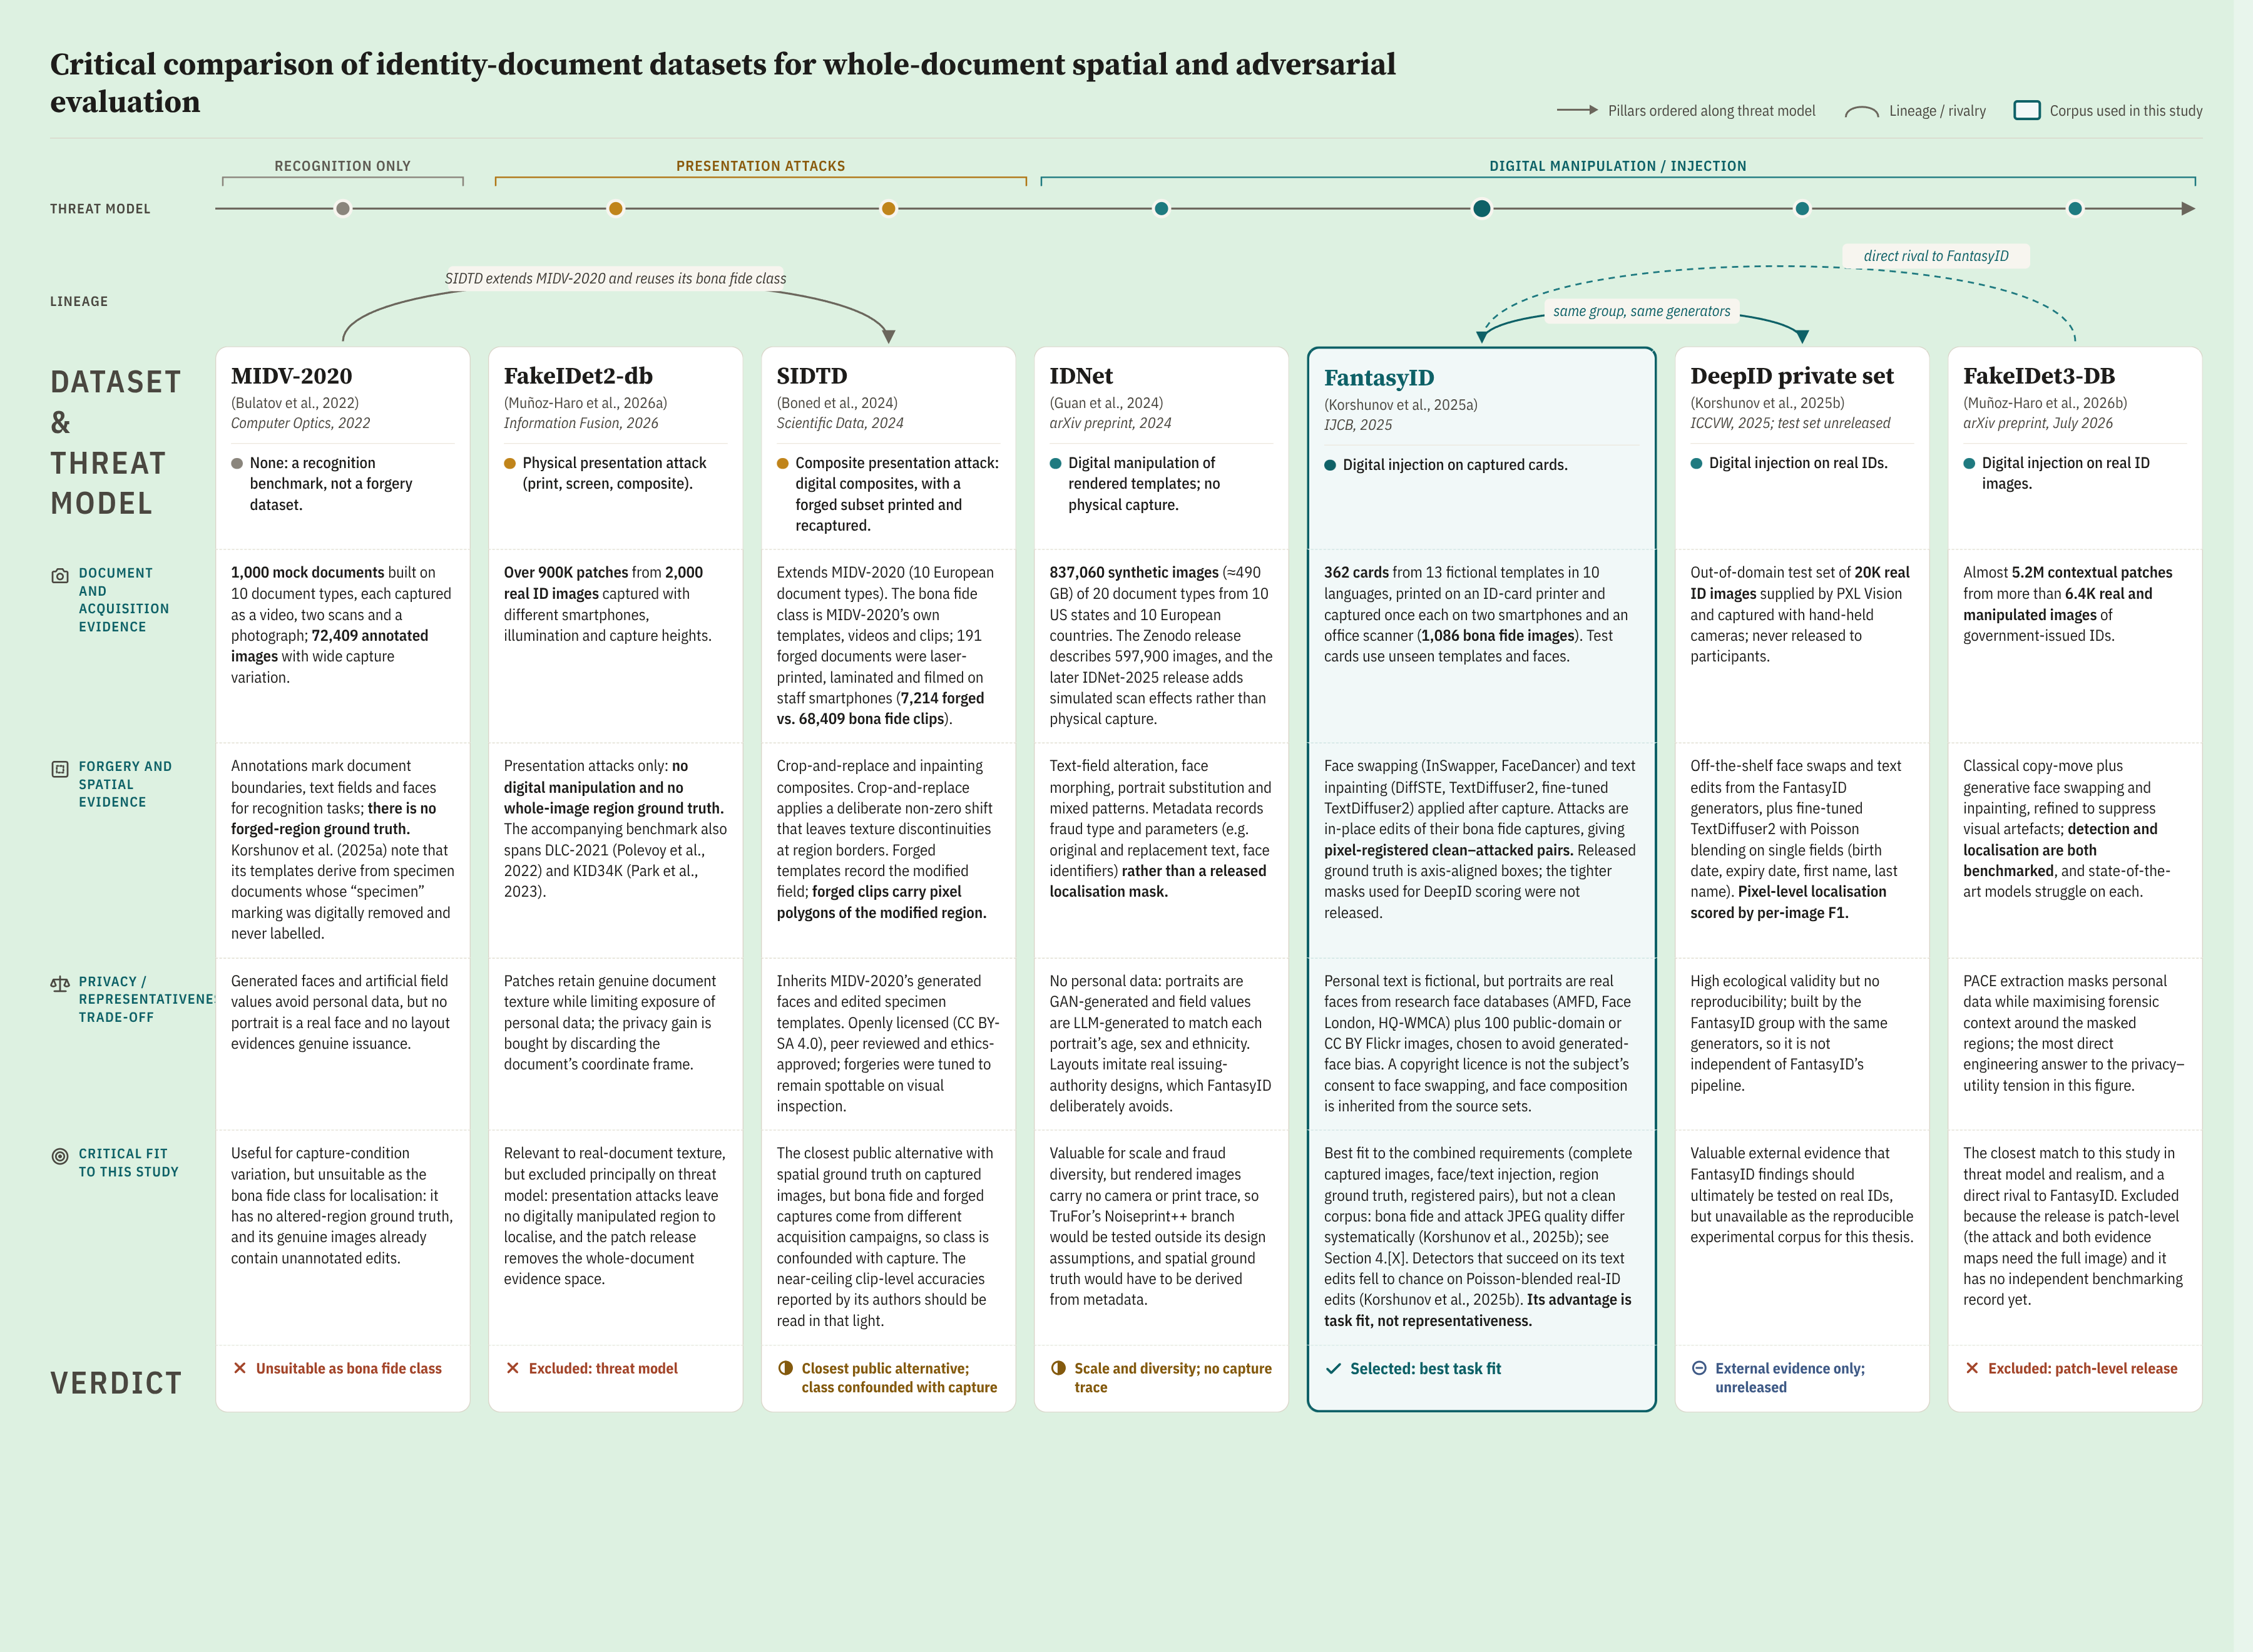
\includegraphics[
%     width=\linewidth,
%     height=0.90\textheight,
%     keepaspectratio
% ]{Images/02Dataset comparison.png}

% \vspace{0.15em}

% \captionof{table}{
% Critical comparison of ID datasets for whole-document spatial and adversarial evaluation.
% }
% \label{tab:lr-datasets}

% \end{center}

% \vfill

% \begin{center}
% \thepage
% \end{center}

% \end{landscape}

% \restoregeometry
% \clearpage
% \clearpage
% Against these requirements, publicly available identity-document datasets make different compromises. Table~\ref{tab:lr-datasets} compares the main alternatives. The comparison is task-specific and a limitation for the present ID spatial study need not be a limitation for the dataset's original purpose.

% \begin{table}[htbp]
% \centering
% \scriptsize
% \renewcommand{\arraystretch}{1.18}
% \caption{Critical comparison of ID datasets for whole-document spatial and adversarial evaluation.}
% \label{tab:lr-datasets}
% \begin{tabularx}{\textwidth}{@{}
% >{\raggedright\arraybackslash}p{0.125\textwidth}
% >{\raggedright\arraybackslash}p{0.19\textwidth}
% >{\raggedright\arraybackslash}p{0.205\textwidth}
% >{\raggedright\arraybackslash}p{0.19\textwidth}
% >{\raggedright\arraybackslash}X@{}}
% \toprule
% Dataset &
% Document and acquisition evidence &
% Forgery and spatial evidence &
% Privacy / representativeness trade-off &
% Critical fit to this study \\
% \midrule

% MIDV-2020
% \citep{bulatov2022midv2020}
% &
% 1,000 mock identity documents represented through photographs, scans and video; more than 72,000 annotated images provide substantial acquisition variation.
% &
% Designed primarily for document detection, recognition, text fields and related analysis rather than paired digital-forgery localisation. Its annotations describe document structure rather than a forged-region ground truth.
% &
% Mock documents and generated identities facilitate public research, but the source documents are artificial and are not evidence of coverage of real issuing authorities.
% &
% Strong evidence for capture-condition robustness, but it cannot directly define the altered region required for DC-DCEC-DCEW evaluation framework.
% \\

% SIDTD
% \citep{boned2024sidtd}
% &
% Extends MIDV-2020 with forged templates and printed/laminated documents captured using smartphones under varied backgrounds and illumination.
% &
% Adds crop-and-replace and inpainting attacks and provides coordinates for modified regions, making it substantially more relevant to localisation than MIDV-2020.
% &
% Retains the privacy advantages of synthetic/mock documents. However, its bona-fide source inherits the characteristics of MIDV-2020, and some crop-and-replace attacks deliberately introduce boundary discontinuities.
% &
% A credible alternative for spatial forgery research. Its manipulation construction and MIDV-derived source images differ from the injection-style face and text manipulations selected for this thesis, so success may partly reflect attack-generation artefacts rather than the intended FantasyID setting.
% \\

% IDNet
% \citep{guan2024idnet}
% &
% Large synthetic benchmark containing hundreds of thousands of identity-document images across multiple US and European document designs.
% &
% Includes text-field replacement, face morphing, portrait substitution and mixed fraud patterns, giving broader semantic fraud coverage than recognition-only datasets.
% &
% Excellent scale and low privacy exposure, but document images and identities are synthetically generated. Scale therefore increases variation without reproducing the same print--capture and sensor-processing history as a photographed physical card.
% &
% Useful for studying diversity, training and cross-layout fraud patterns; less well matched to an experiment where forensic traces from physical capture and subsequent digital manipulation are part of the observed image.
% \\

% FakeIDet2-db
% \citep{munozharo2026fakeidet2}
% &
% More than 900,000 patches derived from approximately 2,000 real ID images acquired under varied smartphone, illumination and capture conditions.
% &
% Supports bona-fide and physical attacks including print, screen and composite presentation attacks; the patch formulation is designed for privacy-aware forensic modelling.
% &
% A major advantage is that patches retain texture originating from real government-issued documents while reducing disclosure of personally identifying content.
% &
% Highly relevant for real-document forensic texture, but the public patch representation removes the complete coordinate system required to ask whether a whole-document evidence map points to the actual manipulated field.
% \\

% FakeIDet3-DB
% \citep{munozharo2026fakeidet3}
% &
% Extends the privacy-aware real-ID approach to millions of contextual patches derived from thousands of real and manipulated ID images.
% &
% Includes classical copy-move and generative manipulations such as face swapping and inpainting, with both detection and localisation evaluation.
% &
% PACE-style extraction seeks to maximise contextual forensic information while suppressing personally identifying information. This directly addresses the privacy--utility tension.
% &
% Closer to the manipulation domain of this thesis than FakeIDet2, but the released representation remains patch-centred rather than a complete-document evidence space. It is also recent preprint evidence and therefore provides less mature benchmarking history.
% \\

% FantasyID
% \citep{korshunov2025fantasyid}
% &
% 362 fictional physical cards across multiple designs and languages are printed and captured using two smartphones and an office scanner, producing 1,086 bona-fide captures.
% &
% Captured images are subsequently subjected to face swapping and text inpainting, including InSwapper, FaceDancer, DiffSTE and TextDiffuser2 variants. Complete images and manipulated-region annotations allow document-level and spatial evaluation.
% &
% Avoids tampering with official government IDs and uses fictional personal information, improving reproducibility and reducing legal/privacy obstacles. It nevertheless uses publicly licensed faces of real people and only a limited set of fictional layouts and capture devices.
% &
% Best alignment with the present conjunction of requirements: complete images, physical capture history, digital face/text manipulation, region ground truth and repeatable clean--attacked comparisons. Its advantage is task fit, not superior population representativeness.
% \\

% DeepID private set
% \citep{korshunov2025deepid}
% &
% Real identity documents are used for a private evaluation set.
% &
% Includes face swapping and text manipulations of specific fields such as birth date, expiry date, first name and last name, providing stronger evidence about realistic field-level attacks.
% &
% Real-document evidence improves ecological relevance but privacy and access constraints prevent public reproduction of the benchmark.
% &
% Valuable external evidence that FantasyID findings should ultimately be tested on real IDs, but unavailable as the reproducible experimental corpus for this thesis.
% \\

% \bottomrule
% \end{tabularx}
% \end{table}

%-----------------------------------------------------------------------------------
%-----------------------------------------------------------------------------------
%-----------------------------------------------------------------------------------
% \begingroup
% \centering
% % \scriptsize
% % \renewcommand{\arraystretch}{1.18}
% \footnotesize
% \renewcommand{\arraystretch}{1.17}

% \begin{xltabular}{\textwidth}{@{}
% >{\raggedright\arraybackslash}p{0.125\textwidth}
% >{\raggedright\arraybackslash}p{0.19\textwidth}
% >{\raggedright\arraybackslash}p{0.205\textwidth}
% >{\raggedright\arraybackslash}p{0.19\textwidth}
% >{\raggedright\arraybackslash}X@{}}

% \caption{Critical comparison of ID datasets for whole-document spatial and adversarial evaluation.}
% \label{tab:lr-datasets}\\

% \toprule
% Dataset &
% Document and acquisition evidence &
% Forgery and spatial evidence &
% Privacy / representativeness trade-off &
% Critical fit to this study \\
% \midrule
% \endfirsthead

% \toprule
% Dataset &
% Document and acquisition evidence &
% Forgery and spatial evidence &
% Privacy / representativeness trade-off &
% Critical fit to this study \\
% \midrule
% \endhead

% \bottomrule
% \endfoot

% MIDV-2020
% \citep{bulatov2022midv2020}
% &
% 1,000 mock identity documents represented through photographs, scans and video; more than 72,000 annotated images provide substantial acquisition variation.
% &
% Designed primarily for document detection, recognition, text fields and related analysis rather than paired digital-forgery localisation. Its annotations describe document structure rather than a forged-region ground truth.
% &
% Mock documents and generated identities facilitate public research, but the source documents are artificial and are not evidence of coverage of real issuing authorities.
% &
% Strong evidence for capture-condition robustness, but it cannot directly define the altered region required for DC-DCEC-DCEW evaluation framework.
% \\
% \midrule

% SIDTD
% \citep{boned2024sidtd}
% &
% Extends MIDV-2020 with forged templates and printed/laminated documents captured using smartphones under varied backgrounds and illumination.
% &
% Adds crop-and-replace and inpainting attacks and provides coordinates for modified regions, making it substantially more relevant to localisation than MIDV-2020.
% &
% Retains the privacy advantages of synthetic/mock documents. However, its bona-fide source inherits the characteristics of MIDV-2020, and some crop-and-replace attacks deliberately introduce boundary discontinuities.
% &
% A credible alternative for spatial forgery research however not chosen as it inherits the limitations of MIDV-2020.
% \\
% \midrule

% IDNet
% \citep{guan2024idnet}
% &
% Large synthetic benchmark containing hundreds of thousands of identity-document images across multiple US and European document designs.
% &
% Includes text-field replacement, face morphing, portrait substitution and mixed fraud patterns, giving broader semantic fraud coverage than recognition-only datasets.
% &
% Excellent scale and low privacy exposure, but document images and identities are synthetically generated. Scale therefore increases variation without reproducing the same print--capture and sensor-processing history as a photographed physical card.
% &
% Useful for studying diversity, training and cross-layout fraud patterns; less well matched to an experiment where forensic traces from physical capture and subsequent digital manipulation are part of the observed image.
% \\
% \midrule

% FakeIDet2-db
% \citep{munozharo2026fakeidet2}
% &
% More than 900,000 patches derived from approximately 2,000 real ID images acquired under varied smartphone, illumination and capture conditions.
% &
% Supports bona-fide and physical attacks including print, screen and composite presentation attacks; the patch formulation is designed for privacy-aware forensic modelling.
% &
% A major advantage is that patches retain texture originating from real government-issued documents while reducing disclosure of personally identifying content.
% &
% Highly relevant for real-document forensic texture, but the public patch representation removes the complete coordinate system required to ask whether a whole-document evidence map points to the actual manipulated field.
% \\
% \midrule

% FakeIDet3-DB
% \citep{munozharo2026fakeidet3}
% &
% Extends the privacy-aware real-ID approach to millions of contextual patches derived from thousands of real and manipulated ID images.
% &
% Includes classical copy-move and generative manipulations such as face swapping and inpainting, with both detection and localisation evaluation.
% &
% PACE-style extraction seeks to maximise contextual forensic information while suppressing personally identifying information. This directly addresses the privacy--utility tension.
% &
% Closer to the manipulation domain of this thesis than FakeIDet2, but the released representation remains patch-centred rather than a complete-document evidence space. It is also recent preprint evidence and therefore provides less mature benchmarking history.
% \\
% \midrule

% FantasyID
% \citep{korshunov2025fantasyid}
% &
% 362 fictional physical cards across multiple designs and languages are printed and captured using two smartphones and an office scanner, producing 1,086 bona-fide captures.
% &
% Captured images are subsequently subjected to face swapping and text inpainting, including InSwapper, FaceDancer, DiffSTE and TextDiffuser2 variants. Complete images and manipulated-region annotations allow document-level and spatial evaluation.
% &
% Avoids tampering with official government IDs and uses fictional personal information, improving reproducibility and reducing legal/privacy obstacles. It nevertheless uses publicly licensed faces of real people and only a limited set of fictional layouts and capture devices.
% &
% Best alignment with the present conjunction of requirements: complete images, physical capture history, digital face/text manipulation, region ground truth and repeatable clean--attacked comparisons. Its advantage is task fit, not superior population representativeness.
% \\
% \midrule

% DeepID private set
% \citep{korshunov2025deepid}
% &
% Real identity documents are used for a private evaluation set.
% &
% Includes face swapping and text manipulations of specific fields such as birth date, expiry date, first name and last name, providing stronger evidence about realistic field-level attacks.
% &
% Real-document evidence improves ecological relevance but privacy and access constraints prevent public reproduction of the benchmark.
% &
% Valuable external evidence that FantasyID findings should ultimately be tested on real IDs, but unavailable as the reproducible experimental corpus for this thesis.
% \\

% \bottomrule
% \end{xltabular}

% \endgroup

%---------------------------------------------

% % \begin{figure}[htbp]
% % \centering
% % \includegraphics[width=0.96\textwidth]{Images/CH02_MassRank_V1.pdf}
% % \caption{Same relevance mass, different rank overlap. Both illustrative maps put 80\% of their mass inside the annotation; one and four of their strongest four pixels fall there, respectively. These are constructed examples, not experimental results.}
% % \label{fig:lr-mass-rank}
% % \end{figure}

% Critical comparison of ID datasets (revised September 2026)
% Requires: booktabs, xltabular, array, natbib, cleveref
% Replace sec:evidence-audit with the label of your Chapter 4 evidence-audit section.
%%%%%%%%%%%%%%%%%%%%%%%%%%SAREVIEW-TABLE-TO-DIAGRAM
% \begingroup
% \centering
% \footnotesize
% \renewcommand{\arraystretch}{1.15}
% \setlength{\tabcolsep}{3.5pt}

% \begin{xltabular}{\textwidth}{@{}
% >{\raggedright\arraybackslash}p{0.105\textwidth}
% >{\raggedright\arraybackslash}p{0.10\textwidth}
% >{\raggedright\arraybackslash}p{0.175\textwidth}
% >{\raggedright\arraybackslash}p{0.19\textwidth}
% >{\raggedright\arraybackslash}p{0.17\textwidth}
% >{\raggedright\arraybackslash}X@{}}

% \caption{Critical comparison of identity-document datasets for whole-document spatial and adversarial evaluation. The line under each dataset name gives its publication status at the time of writing (September 2026).}
% \label{tab:lr-datasets}\\

% \toprule
% Dataset &
% Threat model &
% Document and acquisition evidence &
% Forgery and spatial evidence &
% Privacy / representativeness trade-off &
% Critical fit to this study \\
% \midrule
% \endfirsthead

% \toprule
% Dataset &
% Threat model &
% Document and acquisition evidence &
% Forgery and spatial evidence &
% Privacy / representativeness trade-off &
% Critical fit to this study \\
% \midrule
% \endhead

% \bottomrule
% \endfoot

% MIDV-2020
% \citep{bulatov2022midv2020}
% \newline\textit{Computer Optics, 2022}
% &
% None: a recognition benchmark, not a forgery dataset.
% &
% 1,000 mock documents built on 10 document types, each captured as a video, two scans and a photograph; 72,409 annotated images with wide capture variation.
% &
% Annotations mark document boundaries, text fields and faces for recognition tasks; there is no forged-region ground truth. \citet{korshunov2025fantasyid} note that its templates derive from specimen documents whose ``specimen'' marking was digitally removed and never labelled.
% &
% Generated faces and artificial field values avoid personal data, but no portrait is a real face and no layout evidences genuine issuance.
% &
% Useful for capture-condition variation, but unsuitable as the bona-fide class for localisation: it has no altered-region ground truth, and its genuine images already contain unannotated edits.
% \\
% \midrule

% SIDTD
% \citep{boned2024sidtd}
% \newline\textit{Scientific Data, 2024}
% &
% Composite presentation attack: digital composites, with a forged subset printed and recaptured.
% &
% Extends MIDV-2020 (10 European document types). The bona-fide class is MIDV-2020's own templates, videos and clips; 191 forged documents were laser-printed, laminated and filmed on staff smartphones (7,214 forged vs.\ 68,409 bona-fide clips).
% &
% Crop-and-replace and inpainting composites. Crop-and-replace applies a deliberate non-zero shift that leaves texture discontinuities at region borders. Forged templates record the modified field; forged clips carry pixel polygons of the modified region.
% &
% Inherits MIDV-2020's generated faces and edited specimen templates. Openly licensed (CC BY-SA 4.0), peer reviewed and ethics-approved; forgeries were tuned to remain spottable on visual inspection.
% &
% The closest public alternative with spatial ground truth on captured images, but bona-fide and forged captures come from different acquisition campaigns, so class is confounded with capture. The near-ceiling clip-level accuracies reported by its authors should be read in that light.
% \\
% \midrule

% IDNet
% \citep{guan2024idnet}
% \newline\textit{arXiv preprint, 2024}
% &
% Digital manipulation of rendered templates; no physical capture.
% &
% 837,060 synthetic images ($\approx$490\,GB) of 20 document types from 10 US states and 10 European countries. The Zenodo release describes 597,900 images, and the later IDNet-2025 release adds simulated scan effects rather than physical capture.
% &
% Text-field alteration, face morphing, portrait substitution and mixed patterns. Metadata records fraud type and parameters (e.g.\ original and replacement text, face identifiers) rather than a released localisation mask.
% &
% No personal data: portraits are GAN-generated and field values are LLM-generated to match each portrait's age, sex and ethnicity. Layouts imitate real issuing-authority designs, which FantasyID deliberately avoids.
% &
% Valuable for scale and fraud diversity, but rendered images carry no camera or print trace, so TruFor's Noiseprint++ branch would be tested outside its design assumptions, and spatial ground truth would have to be derived from metadata.
% \\
% \midrule

% FakeIDet2-db
% \citep{munozharo2026fakeidet2}
% \newline\textit{Information Fusion, 2026}
% &
% Physical presentation attack (print, screen, composite).
% &
% Over 900K patches from 2,000 real ID images captured with different smartphones, illumination and capture heights.
% &
% Presentation attacks only: no digital manipulation and no whole-image region ground truth. The accompanying benchmark also spans DLC-2021 \citep{polevoy2022dlc2021} and KID34K \citep{park2023kid34k}.
% &
% Patches retain genuine document texture while limiting exposure of personal data; the privacy gain is bought by discarding the document's coordinate frame.
% &
% Relevant to real-document texture, but excluded principally on threat model: presentation attacks leave no digitally manipulated region to localise, and the patch release removes the whole-document evidence space.
% \\
% \midrule

% FakeIDet3-DB
% \citep{munozharo2026fakeidet3}
% \newline\textit{arXiv preprint, July 2026}
% &
% Digital injection on real ID images.
% &
% Almost 5.2M contextual patches from more than 6.4K real and manipulated images of government-issued IDs.
% &
% Classical copy-move plus generative face swapping and inpainting, refined to suppress visual artefacts; detection and localisation are both benchmarked, and state-of-the-art models struggle on each.
% &
% PACE extraction masks personal data while maximising forensic context around the masked regions; the most direct engineering answer to the privacy--utility tension in this table.
% &
% The closest match to this study in threat model and realism, and a direct rival to FantasyID. Excluded because the release is patch-level (the attack and both evidence maps need the full image) and it has no independent benchmarking record yet.
% \\
% \midrule

% FantasyID
% \citep{korshunov2025fantasyid}
% \newline\textit{IJCB, 2025}
% &
% Digital injection on captured cards.
% &
% 362 cards from 13 fictional templates in 10 languages, printed on an ID-card printer and captured once each on two smartphones and an office scanner (1,086 bona-fide images). Test cards use unseen templates and faces.
% &
% Face swapping (InSwapper, FaceDancer) and text inpainting (DiffSTE, TextDiffuser2, fine-tuned TextDiffuser2) applied after capture. Attacks are in-place edits of their bona-fide captures, giving pixel-registered clean--attacked pairs. Released ground truth is axis-aligned boxes; the tighter masks used for DeepID scoring were not released.
% &
% Personal text is fictional, but portraits are real faces from research face databases (AMFD, Face London, HQ-WMCA) plus 100 public-domain or CC~BY Flickr images, chosen to avoid generated-face bias. A copyright licence is not the subject's consent to face swapping, and face composition is inherited from the source sets.
% &
% Best fit to the combined requirements (complete captured images, face/text injection, region ground truth, registered pairs), but not a clean corpus: bona-fide and attack JPEG quality differ systematically \citep{korshunov2025deepid}; see \cref{sec:evidence-audit}. Detectors that succeed on its text edits fell to chance on Poisson-blended real-ID edits \citep{korshunov2025deepid}. Its advantage is task fit, not representativeness.
% \\
% \midrule

% DeepID private set
% \citep{korshunov2025deepid}
% \newline\textit{ICCVW, 2025; test set unreleased}
% &
% Digital injection on real IDs.
% &
% Out-of-domain test set of 20K real ID images supplied by PXL Vision and captured with hand-held cameras; never released to participants.
% &
% Off-the-shelf face swaps and text edits from the FantasyID generators, plus fine-tuned TextDiffuser2 with Poisson blending on single fields (birth date, expiry date, first name, last name). Pixel-level localisation scored by per-image F1.
% &
% High ecological validity but no reproducibility; built by the FantasyID group with the same generators, so it is not independent of FantasyID's pipeline.
% &
% Valuable external evidence that FantasyID findings should ultimately be tested on real IDs, but unavailable as the reproducible experimental corpus for this thesis.
% \\

% \end{xltabular}

% \endgroup

%--------------------saREVIEW-ENDS----------------------------------

%----------------------------------------------

% Scope paragraph for the body text, placed after Table~\ref{tab:lr-datasets}.
%<sareview>
% Three further groups of datasets were excluded before comparison. 
% \begin{itemize}
%     \item Presentation-attack corpora such as DLC-2021 \citep{polevoy2022dlc2021} and KID34K \citep{park2023kid34k}, together with the private data of the PAD-ID card competitions \citep{tapia2024padid,tapia2025padid2}, address recapture rather than digital manipulation and therefore offer no manipulated region to localise.
%     \item BID \citep{soares2020bid} and FMIDV \citep{alghadi2023fmidv} are unsuitable because their bona-fide images are themselves digitally altered: BID replaces the personal details on real Brazilian identity cards, and FMIDV applies copy-move operations to MIDV-2020 images \citep{korshunov2025fantasyid}.
    
%     \item Finally, the proprietary FREUID dataset \citep{freuid2026}, released under a non-commercial licence for the IJCAI-ECAI 2026 challenge, prints and recaptures digital forgeries across seven Asian and African document types, on the argument that detectors trained on purely digital forgeries rely on artefacts that print-and-capture removes. Its published protocol scores detection only, so it provides no localisation benchmark for this study.
% \end{itemize}


No dataset dominates all of these criteria. A recurring trade-off is visible between \emph{forensic realism} and \emph{privacy-preserving reproducibility}. 

% MIDV-2020 and IDNet make broad public experimentation possible through artificial identities, but their synthetic origins limit the conclusions that can be drawn about real document capture traces. FakeIDet2 and FakeIDet3 move in the opposite direction: they expose forensic texture from real documents while withholding the complete document through privacy-aware patch extraction. This is advantageous for privacy-preserving detector development but conflicts with the present requirement to compare a whole-document spatial map with a known altered region.

% SIDTD sits between these positions. It combines physical recapture with explicitly generated forgeries and modified-region coordinates, making it a meaningful alternative for spatial research \citep{boned2024sidtd}. However, its bona-fide images derive from MIDV-2020 and its crop-and-replace procedure can introduce boundary discontinuities by design. For the present research question, this creates a possible shortcut: a model may learn generation-specific artefacts rather than evidence associated with the manipulated semantic field. This does not invalidate SIDTD, but makes its threat model different from the digital injection setting investigated here.

FantasyID provides the closest conjunction of the required properties. Its fictional cards are physically printed and recaptured before digital manipulation, so the forged samples retain a physical acquisition history while face and text regions are subsequently altered using contemporary generative tools \citep{korshunov2025fantasyid}. It also preserves the complete image and known alteration regions. These properties permit the same forged image to be assessed for the DC-DCEC-DCEW framework of this study.

These strengths come with two cautions from its authors' later work. bona-fide and attacked images differ systematically in JPEG quality, a shortcut a detector can exploit without examining the edited field, which is why Chapter~3 controls compression before training. In the DeepID challenge, detectors that performed well on FantasyID's text edits fell to chance on Poisson-blended edits of real IDs \citep{korshunov2025deepid}. Because DeepID shares FantasyID's authors and generators, this is the strongest available transfer warning rather than independent validation.

% at three levels required by this thesis: whether the detector makes the correct forgery decision, whether its clean spatial evidence agrees with the altered region, and whether an adversary can subsequently degrade that spatial evidence while preserving the decision.

% This selection should not be interpreted as evidence that FantasyID is representative of operational identity verification as a whole. NIST AI RMF and the representativeness principles reflected in the EU AI Act instead expose its principal limitations: a small set of fictional layouts cannot represent the document designs of real issuing authorities, three capture devices cannot span deployment conditions, and repeated captures of the same physical card are not independent observations \citep{nist2023airmf,eu2024aiact}. The dataset is therefore selected for \emph{experimental identifiability and reproducibility}, not for regulatory validation or population-level deployment claims.

% The DeepID challenge provides an important external check on this distinction. Its private evaluation uses real identity documents and includes field-specific face and text manipulations that cannot be reproduced from the public FantasyID corpus \citep{korshunov2025deepid}. The challenge also reports that a participating team observed different JPEG quality factors between bona-fide and manipulated samples. Such a difference is important because a detector could obtain the correct label from processing history rather than from the altered field. The present study therefore does not assume that correct classification establishes forensic validity. A compression-control audit is conducted before spatial eligibility is interpreted.

% Finally, three dataset-specific dependencies are carried forward into the experimental design. First, the available alteration annotations are approximations of the manipulated region rather than perfect semantic ground truth; spatial conclusions therefore require sensitivity checks and more than one measure of agreement. Second, multiple captures derived from the same underlying physical card are dependent observations, so uncertainty estimates and data partitions must respect document stem. Third, fictional documents cannot establish performance across real issuing authorities, nationalities or operational KYC systems. These limitations motivate the mask-sensitivity checks, stem-grouped analysis and restricted external-validity claims defined in Chapter~3 and reported in the subsequent experimental chapters.

Three limitations or risks remain after dataset selection:
\begin{enumerate}
    \item Rectangular annotations approximate the altered regions
    \item Capture variants of one card are dependent observations
    \item Fictional documents cannot establish performance across real issuing authorities.
\end{enumerate}

These motivate mitigating strategies including mask-sensitivity checks, grouping by document stem and restricted claims. Chapter~3 defines these controls, Appendix~A records metric-related risks and the model-specific registers retain preprocessing decisions.

%--------------------------------------------------------------------------------------------------
% \section{Two routes to spatial evidence}
% \label{sec:lr-where}

% \subsection{Post-hoc attribution and ResNet-18 with Grad-CAM}

% Grad-CAM uses gradients of a target score to weight convolutional feature maps, producing a regional indication of class evidence \citep{selvaraju2017gradcam}. It can be applied after classifier training. ResNet-18 supplies an established residual classifier that is manageable for repeated training and attacks \citep{he2016resnet}. This makes the combination a suitable experimental representative without making architecture development part of the research question.

% Other attribution methods offer different trade-offs. Integrated Gradients attributes a prediction relative to a reference input and satisfies explicit sensitivity and implementation-invariance axioms \citep{sundararajan2017axiomatic}. Score-CAM weights activation maps using forward-pass scores instead of gradients \citep{wang2020scorecam}. Neither turns classifier attribution into a supervised forgery mask. Grad-CAM is retained for a focused study of an established method; its selection does not imply that it is the most faithful explainer.

% The explanation target also matters. Finer-CAM contrasts a target class with a reference class to suppress shared features \citep{zhang2025finercam}. This supports explaining the manipulated-minus-bona-fide score difference in a binary classifier. It provides a rationale for that target, not evidence that it will localise document alterations successfully. The exact target and layer belong in Chapter~3 and Appendix~B.

% A coarse feature grid places a further limit on interpretation. Enlarging its map does not restore missing character-level detail. Moreover, a classifier may correctly detect global compression differences, so an attribution outside the edited region need not be an inaccurate account of its behaviour. Clean spatial agreement therefore requires separate assessment before any loss is attributed to an attack.

% \subsection{Native localisation and TruFor}

% TruFor combines RGB information with Noiseprint++, a learned representation of processing traces. Its transformer-based fusion produces a manipulation map and a confidence map; pooled statistics from these maps feed the image-level decision \citep{guillaro2023trufor}. Unlike Grad-CAM, its manipulation output is explicitly trained for localisation. The connection between map and decision makes decision-preserving degradation worth testing, but does not guarantee that one must fail whenever the other fails.

% TruFor has direct precedent as a DeepID baseline. The challenge also demonstrates document-specific adaptation of pretrained forensic models \citep{korshunov2025deepid}. EdgeDoc provides another example of combining forensic traces and visual features for identity documents \citep{george2025edgedoc}. These developments support studying native localisation, while showing that pipeline performance depends on training and adaptation as well as architecture.

% This thesis retains pretrained TruFor as a native baseline. Any fine-tuned condition requires its own clean evaluation; improvement is an empirical question. Training ResNet-18 on documents and using pretrained TruFor does not equalise domain exposure, and fine-tuning both would not equalise their supervision or pretraining. Each pipeline is therefore assessed against its own clean evidence. Shared eligible images provide an additional view, not a basis for attributing differences to architecture alone.


\section{Two routes to spatial evidence}
\label{sec:lr-where}

\subsection{Post-hoc attribution and ResNet-18 with Grad-CAM}

Grad-CAM uses gradients of a target score to weight convolutional feature maps, producing a coarse class-discriminative localisation map \citep{selvaraju2017gradcam}. Because it is applied after classifier training, localisation supervision is not required. ResNet-18 provides an established residual classifier that remains tractable for repeated training and adversarial optimisation \citep{he2016resnet}. The combination therefore provides a conventional classifier--attribution pipeline without making architecture development part of the research question.

Alternative attribution methods represent different design choices. Integrated Gradients is a path-based attribution method that explains a prediction relative to a reference input and satisfies Sensitivity and Implementation Invariance, although its result depends on the baseline \citep{sundararajan2017axiomatic}. Score-CAM represents a forward-pass, perturbation-style CAM alternative that avoids gradient-based weighting but increases computational cost when explanations must be generated repeatedly \citep{wang2020scorecam}. Finer-CAM addresses a different choice namely ``the explanation target'', by contrasting a target class with a reference class to suppress shared features \citep{zhang2025finercam}. None of these alternatives converts classifier attribution into a supervised forgery mask. Grad-CAM is therefore retained as an established and computationally suitable representative, not as a claim that it is the most faithful attribution method.

% Alternative attribution methods change what is gained and what is assumed. Integrated Gradients attributes a prediction relative to a reference input and satisfies Sensitivity and Implementation Invariance, but its result depends on the choice of baseline \citep{sundararajan2017axiomatic}. Score-CAM avoids gradient-based weighting by measuring activation-map contributions through forward passes \citep{wang2020scorecam}; this removes one dependence on gradients but increases computational cost when explanations must be generated repeatedly. Neither method converts classifier attribution into a supervised forgery mask. Grad-CAM is therefore retained as an established and computationally suitable representative, not as a claim that it is the most faithful attribution method.

Finer-CAM does also show that contrasting a target class against a reference class can suppress features shared between classes and expose finer discriminative cues \citep{zhang2025finercam}. This motivates a contrastive manipulated-versus-bona-fide target in the binary classifier, but does not establish that such a map will coincide with the document alteration. The exact target and layer are therefore methodological choices defined in Chapter~3 and Appendix~B.

Spatial resolution imposes a separate limitation. Upsampling a coarse convolutional map cannot recover character-level information absent from its feature grid. More importantly, disagreement with the manipulation mask is not automatically evidence that Grad-CAM inaccurately represents the classifier: a correct decision may genuinely depend on compression or other document-wide cues. Clean spatial agreement must therefore be established separately before adversarial degradation is interpreted.

\subsection{Native localisation and TruFor}

TruFor approaches the problem differently. It combines RGB features with Noiseprint++, a learned representation of camera and processing traces, through transformer-based fusion \citep{guillaro2023trufor}. It produces an anomaly map and an associated confidence map; confidence-weighted pooling summarises these outputs before a classifier produces the image-level integrity score. Unlike Grad-CAM, localisation is therefore an explicitly trained component of the forensic pipeline. This structural connection makes decision-preserving spatial degradation a stronger constraint, while still leaving open whether substantial map changes can occur without changing the final decision.

% TruFor is not the only native-localisation alternative. DeepID used it as a baseline and showed that document-specific adaptation of forensic models can improve performance \citep{korshunov2025deepid}. EdgeDoc goes further by combining a lightweight visual transformer with noiseprint features specifically for identity-document forgery detection and localisation \citep{george2025edgedoc}. Such systems may be better adapted to this domain, but using them would also introduce additional task-specific training and supervision into the comparison.

Similar to post-hoc attribution, Native localisation also has alternatives offering different design choices. TruFor represents a general-purpose forensic model with explicit manipulation localisation, while DeepID demonstrates document-specific adaptation of pretrained forensic models \citep{korshunov2025deepid}. EdgeDoc represents a more directly domain-adapted alternative by combining visual and forensic-trace features specifically for identity-document forgery detection and localisation \citep{george2025edgedoc}. Such systems may benefit from task-specific training, but adopting them would also change the amount and type of domain supervision in the comparison. TruFor is therefore retained as a pretrained native-localisation baseline rather than as the strongest possible document-specific model.

A document-trained ResNet-18 and pretrained TruFor do not have equal domain exposure, but fine-tuning both would not equalise their objectives, pretraining or supervision either. Architecture-level ranking would consequently be misleading. Each pipeline is evaluated against its own clean evidence, while results on shared eligible images provide a controlled supplementary comparison rather than evidence that one architecture is intrinsically superior.



% \section{What should count as acceptable spatial evidence?}
% \label{sec:lr-metrics}

% \subsection{Spatial agreement and explanation faithfulness}

% A visually convincing map can be misleading. Randomisation tests show that some saliency methods retain structure after learned model information is disrupted \citep{adebayo2018sanity}. Such tests assess dependence on the model; annotation overlap asks a different question. A map may reflect a classifier's reliance on a shortcut accurately while offering little help in finding the alteration. Here, ``evidence correct'' means meeting a declared spatial-agreement criterion. It is not a general certificate of explanation quality.

% Pixel-F1 and intersection-over-union are appropriate for evaluating predicted segmentation masks. TruFor reports F1 with a fixed threshold and with the best threshold for each image \citep{guillaro2023trufor}. The latter uses ground truth unavailable during deployment. Applying an arbitrary probability threshold to Grad-CAM is also problematic because its values are relative attribution strengths. F1 and IoU remain useful localisation diagnostics, but a common primary criterion should accommodate both kinds of continuous map.

% \subsection{Relevance mass and relevance rank}

% Score-CAM evaluates how much saliency energy falls inside an annotated region \citep{wang2020scorecam}. CLEVR-XAI defines relevance mass accuracy and relevance rank accuracy for evaluating non-negative explanation maps against ground truth \citep{arras2022clevrxai}. These provide the literature basis for the two quantities used here.

% Let $S(p)$ be the non-negative spatial value at pixel $p$, $M$ the union of annotated manipulation regions, and $\Omega$ the valid document area. With $K=|M|$, the measures are
% \begin{equation}
% E=\frac{\sum_{p\in M}S(p)}{\sum_{p\in\Omega}S(p)},
% \qquad
% \mathrm{RRA}=\frac{|\operatorname{TopK}_{K}(S)\cap M|}{K}.
% \label{eq:lr-mass-rank}
% \end{equation}
% The top-$K$ pixels are selected within $\Omega$. Both measures range from zero to one for valid maps and non-empty masks.

% $E$ asks how much of the map's total mass lies inside the annotation. RRA asks how many of its strongest pixels fall there when the selected set has the same area as the annotation. Figure~\ref{fig:lr-mass-rank} shows why these questions differ: identical mass containment can accompany very different rank overlap. RRA adds a check on the spatial distribution of strong evidence, although it does not prove that every altered feature has been identified.

% %<sareview>
% % \begin{figure}[htbp]
% % \centering
% % \includegraphics[width=0.96\textwidth]{Images/CH02_MassRank_V1.pdf}
% % \caption{Same relevance mass, different rank overlap. Both illustrative maps put 80\% of their mass inside the annotation; one and four of their strongest four pixels fall there, respectively. These are constructed examples, not experimental results.}
% % \label{fig:lr-mass-rank}
% % \end{figure}

% The transfer from CLEVR-XAI needs qualification. Its controlled visual-question-answering setting can identify relevant objects by construction. An identity-document annotation identifies an edited region, which need not contain every cue used by a forgery classifier. Applying the measures to TruFor also evaluates the distribution of manipulation scores, rather than classifier relevance. The equations provide common spatial measurements without making the maps equivalent explanations.

% \subsection{Why two measures still need supporting checks}

% Neither measure removes region-size effects. If $A=|M|/|\Omega|$, a uniform map gives $E=A$. The area-normalised quantity $\mu_w=E/A$ is consequently useful as a diagnostic, but can be large when little total evidence lies inside a small region. For example, $A=0.01$ and $E=0.02$ give $\mu_w=2$, although 98\% of the mass remains outside. A mass requirement is therefore still needed.

% RRA also depends on annotation size and geometry. Under spatially random ranking its expected value is $A$; its top-$K$ boundary can be sensitive to tied values. Both measures are unchanged by multiplying a valid map by a positive constant, so they describe spatial allocation rather than absolute confidence. Zero or invalid maps need explicit handling, not arbitrary normalisation. Interpolation, padding and broad rectangles can further affect both scores.

% The Pointing Game checks whether the strongest location falls inside the target region \citep{zhang2016excitation}. It is easy to interpret, but one successful pixel cannot establish regional agreement. PG, $A$, $\mu_w$ and face/text measurements therefore remain supporting diagnostics. A union mask can also hide uneven performance: a large portrait region may dominate while a small text edit receives little evidence. Component-level measurements and visual examples help expose this limitation. Chapter~4 also retains continuous $E$ and RRA values: averages alone cannot identify which individual images satisfy both requirements.

% The literature supplies these measures, but does not establish a universal threshold for acceptable evidence in this task. This study combines $E\geq\tau_E$ and $\mathrm{RRA}\geq\tau_{\mathrm{RRA}}$. The thresholds require calibration from clean development data, supported by visual judgements made without seeing the numerical metrics. The same procedure applies to both pipelines, while numerical thresholds may differ. Chapter~3 specifies selection and freezing; Appendix~A records the rating scheme, alternatives, tie handling, boundary sensitivity and calibration uncertainty. A visual judgement remains a fallible reference, and calibration agreement is not independent validation.

%%%%%%%%%%%%%%%%%%%%%%%%%%%%%%%%version 02 %%%%%%%%%%%%%%%%%%%%%%%%%%%%%%%%%%%%%%%%%%

% \section{What should count as acceptable spatial evidence?}
% \label{sec:lr-metrics}

% \subsection{Spatial agreement is not explanation faithfulness}

% A spatial map can look convincing without reflecting what the model has learned. Randomisation tests show that some saliency methods produce near-identical maps even after the model's parameters are randomised \citep{adebayo2018sanity}. Those tests are about faithfulness to the model. Comparing a map with the manipulation mask, which marks where the forgery was made, asks a different question. It evaluates if the displayed evidence fall where the alteration occurred? The two can diverge, because a classifier may faithfully rely on compression, acquisition or other shortcut cues outside the edited field. For this reason, ``acceptable spatial evidence'' therefore means meeting a declared spatial-agreement rule, not providing a complete or causally faithful explanation.

% Standard segmentation measures, the obvious candidates, are also an awkward common gate. Pixel-F1 and intersection-over-union suit binary regions, and TruFor reports F1 at both a fixed threshold and the best per-image threshold \citep{guillaro2023trufor}. \citep{guillaro2023trufor}. The second is chosen using ground truth, which no deployed system has, introducing a significant validation pitfall where test-stage optimization overestimates real-world utility \citep{maier2024metrics}. Grad-CAM, meanwhile, gives relative attribution strengths, not calibrated manipulation probabilities, so one numerical threshold would mean different things in each pipeline. F1 and IoU remain useful diagnostics, but the primary criterion should compare continuous, non-negative maps without binarising them first.

% \subsection{Why relevance mass and relevance rank are combined}

% Score-CAM motivates measuring the proportion of saliency energy inside a target region \citep{wang2020scorecam}, while CLEVR-XAI formalises complementary relevance mass accuracy(RMA) and relevance rank accuracy(RRA) for non-negative maps \citep{arras2022clevrxai}. Let $S(p)$ be the spatial value at pixel $p$, $M$ the union of annotated manipulation regions, $\Omega$ the valid document area, and $K=|M|$:
% \begin{equation}
% E=\frac{\sum_{p\in M}S(p)}{\sum_{p\in\Omega}S(p)},
% \qquad
% \mathrm{RRA}=\frac{|\operatorname{TopK}_{K}(S)\cap M|}{K}.
% \label{eq:lr-mass-rank}
% \end{equation}

% The two measures address different failure modes. 
% \begin{itemize} [itemsep=1pt]
%     \item $E$ asks how much total map mass lies inside the alteration, but does not require the strongest responses to be concentrated there.
%     \item RRA asks whether the highest-ranked pixels occupy the alteration, but ranking alone does not ensure that it receives a substantial share of total evidence.
% \end{itemize}
% Their conjunction is therefore more defensible than either measure alone. This motivates DCEC: among samples already satisfying decision correctness (DC), clean evidence is accepted only when both $E\geq\tau_E$ and $\mathrm{RRA}\geq\tau_{\mathrm{RRA}}$.

% The transfer from CLEVR-XAI still needs qualification for this study. Its relevant objects can be specified by construction because an ID-document mask marks edited pixels, not necessarily every cue legitimately used by a forgery detector. 
% The equations also have different semantics across pipelines: 
% \begin{itemize} [itemsep=0pt]
%     \item For Grad-CAM, they measure class attribution
%     \item For TruFor, they measure a learned manipulation score.
% \end{itemize}
% Hence it is clear that they provide a common test of spatial agreement, not equivalent explanations in line with the study's objective.

% \section{What should count as acceptable spatial evidence?}
% \label{sec:lr-metrics}

% \subsection{Spatial agreement is not explanation faithfulness}

% A spatial map can look convincing without reflecting what the model has learned. Randomisation tests show that some saliency methods retain substantial structure after learned model parameters are disrupted \citep{adebayo2018sanity}. Such tests concern faithfulness to the model, whereas comparison with a manipulation mask asks whether displayed evidence coincides with the known alteration. The two need not agree. A classifier may faithfully rely on compression, acquisition or other shortcut cues outside the edited field. ``Acceptable spatial evidence'' in this thesis therefore concerns spatial agreement with the manipulation rather than a claim of explanation faithfulness.

% Standard segmentation measures are also an awkward common criterion. Pixel-F1 and intersection-over-union suit binary regions, and TruFor reports F1 using both a fixed threshold and a best per-image threshold \citep{guillaro2023trufor}. The latter uses ground truth to optimise the reported result, while Grad-CAM produces relative attribution strengths rather than calibrated manipulation probabilities. Applying one numerical threshold would therefore impose different assumptions on the two pipelines. F1 and IoU remain relevant localisation measures, but continuous-map measures avoid making binarisation the primary basis of comparison.

% \subsection{Why relevance mass and relevance rank are combined}

% Score-CAM considers the proportion of saliency energy falling within an annotated region \citep{wang2020scorecam}, while CLEVR-XAI formalises relevance mass accuracy (RMA) and relevance rank accuracy (RRA) for evaluating non-negative explanation maps against ground-truth regions \citep{arras2022clevrxai}. Let $S(p)$ denote the non-negative spatial value at pixel $p$, $M$ the annotated region and $K=|M|$:
% \begin{equation}
% E=\frac{\sum_{p\in M}S(p)}{\sum_{p}S(p)},
% \qquad
% \mathrm{RRA}=\frac{|\operatorname{TopK}_{K}(S)\cap M|}{K}.
% \label{eq:lr-mass-rank}
% \end{equation}

% The measures test different properties. Relevance mass asks how much of the total spatial response lies within the target, whereas rank accuracy asks whether the strongest responses preferentially occupy it. CLEVR-XAI treats these as complementary rather than interchangeable measures \citep{arras2022clevrxai}: a map may concentrate substantial total mass inside a region without ranking its pixels most strongly, or achieve high-ranked overlap while distributing considerable mass elsewhere. For this study, that complementarity provides the literature basis for requiring both containment and concentration when defining acceptable clean spatial evidence.

% Their transfer to identity-document forgery nevertheless requires caution. CLEVR-XAI uses synthetic visual-question-answering scenes in which relevant objects can be specified by construction. A manipulation mask instead identifies where an edit occurred; it does not prove that all legitimate forensic evidence must originate there. The meaning also differs by pipeline: Grad-CAM expresses class attribution, whereas TruFor produces learned manipulation scores. RMA and RRA therefore create a common spatial comparison, not a claim that the two maps are equivalent explanations.

% \subsection{Limitations of spatial agreement metrics}

% No localisation metric is neutral to its evaluation setting. CLEVR-XAI reports changes in relevance accuracy when target-object size and prediction confidence are varied, showing that measured explanation quality also reflects properties of the evaluated sample \citep{arras2022clevrxai}. More broadly, Tomsett et al.\ show that saliency metrics can give inconsistent assessments and that implementation choices can materially affect conclusions \citep{tomsett2020sanitymetrics}. Metric choice should therefore follow the question being asked rather than assume that one score represents explanation quality generally.

% Region-based ground truth creates particular difficulties for identity documents. Large portrait alterations and very small text edits differ greatly in area, so apparent spatial agreement can partly reflect target size. Rectangular annotations may also contain unchanged pixels, while a union of several regions can conceal poor localisation of a smaller component. These effects are especially relevant where face and text manipulations coexist and argue against interpreting a single aggregate score without supporting evidence.

% Simpler alternatives illustrate the same trade-off. The Pointing Game asks only whether the maximum response lies inside the annotated region \citep{zhang2016excitation}; it is intuitive but ignores the remainder of the map, so one correctly placed peak cannot establish regional agreement. Conversely, overlap measures assess a broader region but require thresholding. The literature therefore supports using complementary spatial properties rather than treating any one localisation measure as a universal definition of acceptable evidence.

% For this thesis, these findings provide the conceptual basis for distinguishing a correct document decision (DC) from a correct decision whose clean spatial evidence is also acceptable (DCEC). The operational definition of DCEC, threshold calibration, supporting diagnostics and the subsequent decision-preserving adversarial failure condition are methodological choices and are specified in Chapter~3.


% \subsection{Calibration, baselines and supporting checks}

% Region size remains a confound. If $A=|M|/|\Omega|$, a uniform map gives $E=A$, and random ranking has expected RRA $A$. The area-normalised ratio $\mu_w=E/A$ therefore indicates enrichment above this baseline, but cannot replace $E$: a small region can obtain a large ratio while containing little total mass. The Pointing Game tests whether the strongest location lies inside the target \citep{zhang2016excitation}, but one successful pixel cannot establish regional agreement. $A$, $\mu_w$, Pointing Game, component-level face/text scores and visual examples therefore remain supporting diagnostics.

% Mask geometry and implementation also matter as they carry an inherent risk. Rectangular annotations may include unchanged pixels; a union mask can let a large portrait dominate a small text edit; ties affect the top-$K$ boundary; and interpolation, padding or invalid maps require explicit handling. Continuous $E$ and RRA values are therefore retained alongside pass/fail status.

% The literature does not provide universal thresholds for acceptable ID-document evidence. Thresholds are calibrated on clean development data with visual judgements made without access to the numerical scores, then frozen before adversarial evaluation. The procedure is common across pipelines, although numerical thresholds may differ because map semantics and distributions differ. DCEC is therefore a pipeline-specific clean eligibility condition rather than a universal quality scale, so its coverage must be reported. DCEW is counted only when an initially DCEC sample retains the correct forgery decision after attack but fails at least one frozen evidence condition. This prevents already-poor clean maps from inflating apparent adversarial vulnerability. Chapter~3 defines calibration and freezing; Appendix~A records the rating scheme and sensitivity checks.

%--------------------------------------version 03----------------------------------------------

\section{What should count as acceptable spatial evidence?}
\label{sec:lr-metrics}

\subsection{Spatial agreement is not explanation faithfulness}

A spatial map can look convincing without reflecting what the model has learned. Randomisation tests show that some saliency methods retain substantial structure after learned parameters are disrupted \citep{adebayo2018sanity}. Such tests concern faithfulness to the model; comparison with a manipulation mask asks whether displayed evidence coincides with the known alteration. The two can diverge because a classifier may faithfully rely on compression, acquisition or other shortcut cues outside the edited field. Here, ``acceptable spatial evidence'' therefore means spatial agreement with the alteration, not a general certificate of explanation faithfulness.

Standard segmentation measures are also an awkward common criterion. Pixel-F1 and intersection-over-union suit binary regions, while TruFor reports F1 using both a fixed threshold and a best per-image threshold \citep{guillaro2023trufor}. Grad-CAM instead produces relative attribution strengths rather than calibrated manipulation probabilities. A common threshold would therefore impose different assumptions on the two pipelines. F1 and IoU remain useful diagnostics, but continuous-map measures avoid making binarisation the primary basis of comparison.

\subsection{Why relevance mass and relevance rank are combined}

Score-CAM considers the proportion of saliency energy inside an annotated region \citep{wang2020scorecam}, while CLEVR-XAI formalises relevance mass accuracy (RMA), written E below and relevance rank accuracy (RRA) for non-negative maps \citep{arras2022clevrxai}. Let $S(p)$ be the spatial value at pixel $p$, $M$ the annotated manipulation region, and $K=|M|$:
\begin{equation}
E=\frac{\sum_{p\in M}S(p)}{\sum_{p}S(p)},
\qquad
\mathrm{RRA}=\frac{|\operatorname{TopK}_{K}(S)\cap M|}{K}.
\label{eq:lr-mass-rank}
\end{equation}

The measures test different properties. 
\begin{itemize}
    \item $E$ asks how much total map mass lies inside the alteration
    \item RRA asks whether the strongest responses preferentially occupy it.
\end{itemize}
A map can perform well on one while remaining weak on the other, so their combination provides a stronger basis for judging clean spatial evidence than either alone.

Their transfer from CLEVR-XAI nevertheless needs qualification. Its relevant objects are known by construction, whereas an ID-document mask marks where an edit occurred, not necessarily every cue legitimately used by a detector. 
The map semantics also differ: 
\begin{itemize}
    \item Grad-CAM expresses class attribution
    \item TruFor produces learned manipulation scores.
\end{itemize}
The measures therefore provide a common test of spatial agreement, not equivalent explanations.

\subsection{Limitations of spatial agreement metrics}

No localisation metric is independent of its evaluation setting as discussed below. 
\begin{enumerate}
    \item CLEVR-XAI reports changes in relevance accuracy with target size, while broader work shows that saliency metrics can disagree and that implementation choices can alter conclusions \citep{arras2022clevrxai,tomsett2020sanitymetrics}. This is important for identity documents, where a large portrait replacement and a small text edit differ greatly in area.
    \item Simpler alternatives have complementary weaknesses. The Pointing Game asks only whether the maximum response lies inside the target \citep{zhang2016excitation}; one successful peak cannot establish regional agreement.
    \item Conversely, overlap measures require thresholding. Rectangular or union annotations can also conceal uneven localisation across components.
\end{enumerate}

The literature therefore supports combining spatial properties rather than treating one score as a universal definition of evidence quality. These findings provide the conceptual basis for separating a correct decision (DC) from a correct decision with acceptable clean spatial evidence (DCEC). The operational definition of DCEC, threshold calibration, supporting diagnostics and the later decision-preserving adversarial failure condition are specified in Chapter~3.


%------------------------------------------------------------------------------------
% \section{Attacking explanations while preserving decisions}
% \label{sec:lr-xai-attacks}

% \citet{ghorbani2019fragile} show that small input changes can substantially alter neural-network explanations while retaining the predicted label. \citet{dombrowski2019explanations} relate this sensitivity to network geometry and steer explanations towards chosen targets while keeping outputs approximately constant. Together, these studies establish that prediction stability does not ensure explanation stability. However, a changed map is not necessarily a worse map: similarity to the clean output does not itself measure agreement with a known manipulation.

% \citet{heo2019fooling} demonstrate a different route by changing model parameters so that explanations become misleading while predictive performance is largely retained. This establishes a model-owner threat, which must be distinguished from the bounded input perturbations considered here. Combining their outcomes into one attack-success comparison would conceal differences in attacker capability.

% More recent work extends prediction-preserving manipulation to audio deepfake explanations \citep{kitlowski2026fragility}. Its study of 100 recordings supports the relevance of the failure to forensic systems, but audio-specific perceptual constraints and map-similarity measures do not answer the identity-document question. These studies motivate an adversary targeting spatial evidence and a success rule that verifies the final decision, rather than trusting a decision-preservation term in the optimisation loss.


\section{Attacking spatial evidence while preserving forgery decisions}
\label{sec:lr-xai-attacks}

\citet{ghorbani2019fragile} show that small input perturbations can alter attribution maps while preserving the predicted label. \citet{dombrowski2019explanations} steer explanations towards chosen targets and relate the effect to network geometry. Together they establish the separation used here: prediction stability does not imply spatial-evidence stability. Their experiments concern generic image classification and mainly measure departure from the clean explanation. 
% % In identity documents, however, the manipulation region is known and may range from a few characters to an entire portrait; degradation can therefore be judged against the forgery while the document remains correctly classified as forged.
% In the controlled benchmark setting used here, the manipulated region is known from dataset annotations and may range from a few altered characters to an entire portrait. This makes it possible to evaluate whether an attack moves spatial evidence away from the true edit while the document is still correctly classified as forged; such ground truth would not ordinarily be available during deployment.

In the controlled benchmark setting used here, dataset annotations identify the true manipulated region, which may range from a few characters to an entire portrait. This allows spatial degradation to be measured against the actual edit while the forgery decision is preserved, even though such ground truth is unavailable in deployment.

\citet{heo2019fooling} instead modify model parameters to mislead explanations while retaining predictive performance. This is a model-owner threat, distinct from a bounded input-space adversary. Audio-deepfake work extends prediction-preserving explanation attacks to a forensic task, but uses domain-specific perceptual constraints and map-similarity objectives \citep{kitlowski2026fragility}.

Within the identity-document literature reviewed here, work has focused on detection and localisation rather than deliberately degrading initially acceptable spatial evidence while preserving the forgery decision \citep{korshunov2025fantasyid,korshunov2025deepid,kumar2026flid}. This motivates testing both post-hoc attribution and native localisation, measuring degradation against the known manipulation rather than map change alone, and conditioning adversarial failure on acceptable clean evidence.

%------------------------------------------------------------------------------------
\section{Attacking forensic and document localisers}
\label{sec:lr-loc-attacks}

\citet{cao2024transferable} demonstrate optimisation- and gradient-based attacks on image-tampering localisers, including transfer between models. \citet{zeng2024frequency} introduce frequency-constrained attacks to improve transferability. Their results establish vulnerabilities in spatial forensic prediction, but neither supplies this study's joint test of acceptable clean evidence followed by its loss under a preserved image-level decision.

Document-specific adversarial robustness has also begun to receive attention. \citet{shao2024documentrobustness} evaluate attacks on DocTamper and T-Sroie and propose manifold-based adversarial training. Their experiments show localisation degradation and improvements from defensive training. This is a closer domain precedent than natural-image attacks: sparse tampered pixels and weak forensic features affect both the attack and its evaluation. However, their segmentation-focused study does not evaluate Grad-CAM and TruFor through a clean DCEC population with a preserved document-level forgery verdict. The remaining gap is consequently narrower than adversarial robustness of documents in general.

Projected-gradient methods provide a way to search within a declared perturbation budget \citep{madry2018towards}. It should be noted that a budget only bounds pixel changes and does not by itself prove imperceptibility or realistic access to a deployed service. Evaluation guidance also warns that weak attacks and unusable gradients can produce misleading robustness claims \citep{carlini2019evaluating}. White-box evaluation is therefore a controlled stress test. Successful attacks establish vulnerability under the tested conditions; unsuccessful attempts do not certify robustness. This evaluation literature therefore motivates explicit attack-strength and gradient-validity checks in the methodology, without treating successful localisation degradation as evidence of a practical verification bypass.

% \section{Synthesis: from DC to DCEC to DCEW}
% \label{sec:lr-gap}

% The reviewed work establishes three points: explanation maps can change with the prediction intact; forensic localisation can fail under attack; and spatial agreement needs more than a visually plausible heatmap. Table~\ref{tab:lr-gap} connects these findings to the remaining evaluation need.

% \begin{table}[htbp]
% \centering
% \small
% \renewcommand{\arraystretch}{1.15}
% \caption{How the reviewed evidence informs this study. The remaining needs refer to the selected research question, not universal absences from the literature.}
% \label{tab:lr-gap}
% \begin{tabularx}{\textwidth}{@{}>{\raggedright\arraybackslash}p{0.28\textwidth}>{\raggedright\arraybackslash}X>{\raggedright\arraybackslash}X@{}}
% \toprule
% Evidence & What it establishes & Need carried forward \\
% \midrule
% Explanation attacks \citep{ghorbani2019fragile,dombrowski2019explanations} & Maps can change while predictions remain stable. & Measure loss of annotation agreement. \\
% Localiser attacks \citep{cao2024transferable,shao2025documentrobustness} & Forensic and document masks are attackable. & Verify preservation of the document decision. \\
% Spatial evaluation \citep{wang2020scorecam,arras2022clevrxai} & Mass and rank describe different properties. & Calibrate a joint evidence-acceptance rule. \\
% This study & Evaluates the selected pipelines on eligible document images. & Report conditional degradation alongside coverage and uncertainty. \\
% \bottomrule
% \end{tabularx}
% \end{table}

% DC first identifies manipulated images correctly classified on clean input. DCEC retains those whose maps pass both evidence requirements. Within this fixed clean set, DCEW requires the adversarial decision to remain correct while either requirement fails. Classification flips remain in the original DCEC denominator and are reported separately. This distinguishes the intended failure from ordinary decision evasion and from evidence that was already inadequate.

% Restricting attention to DCEC creates a selection risk: a large conditional attack rate may describe only a small part of the dataset. Reporting the full evaluation scope, DC and DCEC counts by pipeline and forgery family keeps that limitation visible. Where attacks already cover the broader DC population, DCEC analysis selects the corresponding paired outputs. It describes an analysis population, not a requirement to regenerate attacks.

% The primary population is each pipeline's own DCEC set. Their intersection supplies additional within-pipeline degradation estimates and shared visual examples. It reduces variation in image composition, but does not remove differences in training, map meaning or clean performance. Uncertainty must also respect repeated document stems. These choices support an evaluation of conditional vulnerability, rather than an architecture ranking.

% \section{Conclusion}
% \label{sec:lr-conclusion}

% The literature supports studying spatial evidence separately from detection accuracy. FantasyID provides suitable annotated document images, while ResNet-18/Grad-CAM and TruFor offer two distinct forms of spatial output. Established mass and rank measures support the proposed acceptance rule, with explicit limits on what it means. The contribution is their use in a documented evaluation of decision-preserving evidence loss, accompanied by clean coverage, continuous degradation and uncertainty. Chapter~3 translates this rationale into the research protocol; Chapters~4 and~5 report the clean and adversarial evidence.

%%%---------------------------- version 01----------------------------------------
% \section{Synthesis and research gap}
% \label{sec:lr-gap}

% The reviewed literature establishes several parts of the problem separately. Identity-document research shows that forgeries may affect semantically important regions ranging from small text fields to complete portraits, and that detection and localisation should therefore be distinguished. Attribution research shows that a classifier's spatial explanation can change while its predicted class remains unchanged \citep{ghorbani2019fragile,dombrowski2019explanations}. Forensic-localisation studies further show that manipulation maps themselves can be degraded adversarially \citep{cao2024transferable,shao2024documentrobustness}. Finally, spatial-evaluation research shows that no single localisation measure captures all desirable properties of a continuous evidence map \citep{wang2020scorecam,arras2022clevrxai}.

% These strands do not, however, answer the research question posed in Chapter~1 when combined in the identity-document setting. Explanation attacks have largely been studied as changes to generic classifier explanations, while forensic-localiser attacks primarily evaluate degradation of localisation outputs. Identity-document studies concentrate on detecting or localising the underlying forgery. Within the literature reviewed here, there is limited evidence on whether an adversary can start from a forged document that is both correctly detected and already has acceptable spatial evidence, then degrade that evidence while preserving the correct forgery verdict. This distinction matters because an attack on an already poor map does not demonstrate loss of useful evidence, and a change of the document decision is ordinary evasion rather than the failure considered here.

% \begin{table}[htbp]
% \centering
% \small
% \renewcommand{\arraystretch}{1.15}
% \caption{Synthesis of the literature relative to the research question.}
% \label{tab:lr-gap}
% \begin{tabularx}{\textwidth}{@{}
% >{\raggedright\arraybackslash}p{0.25\textwidth}
% >{\raggedright\arraybackslash}X
% >{\raggedright\arraybackslash}X@{}}
% \toprule
% Literature strand & What is established & What remains unresolved for this research question \\
% \midrule

% Identity-document forensics
% \citep{korshunov2025fantasyid,korshunov2025deepid}
% &
% Forgery detection and localisation are distinct tasks, with manipulations ranging from small text edits to large portrait changes.
% &
% Whether spatial evidence that is initially useful can be selectively degraded while the document remains correctly identified as forged.
% \\

% Post-hoc explanation attacks
% \citep{ghorbani2019fragile,dombrowski2019explanations}
% &
% Attribution maps can be changed substantially without necessarily changing the predicted class.
% &
% Whether this instability corresponds to loss of agreement with the true alteration in an identity-document forgery task.
% \\

% Forensic-localiser attacks
% \citep{cao2024transferable,shao2024documentrobustness}
% &
% Learned manipulation-localisation outputs are vulnerable to bounded adversarial perturbations.
% &
% Whether comparable decision-preserving evidence loss occurs when localisation contributes directly to a forgery-detection pipeline.
% \\

% Spatial evaluation
% \citep{wang2020scorecam,arras2022clevrxai}
% &
% Mass and rank capture complementary properties of continuous spatial maps.
% &
% How to distinguish genuine loss of initially acceptable evidence from changes to maps that were already spatially inadequate.
% \\

% \bottomrule
% \end{tabularx}
% \end{table}

% The resulting gap is therefore narrower than adversarial robustness, explanation fragility or document localisation considered independently. The unresolved question concerns their intersection: the \emph{extent} to which bounded perturbations can degrade initially acceptable spatial evidence from two different routes---post-hoc attribution and native localisation---without removing the correct identity-document forgery decision. The DC--DCEC--DCEW distinction provides the conceptual framing for that question: decision correctness, acceptable clean evidence, and subsequent decision-preserving evidence loss are treated as different states. Their operational definitions and experimental implementation are specified in Chapter~3.

% The five objectives in Chapter~1 follow from this synthesis. O1 establishes what clean detection and spatial evidence each pipeline can support; O2 addresses whether that evidence is credible enough to form a clean starting population; O3 tests the central decision-preserving adversarial failure; O4 determines its extent while accounting for pipeline coverage and uncertainty; and O5 interprets what those findings imply for the use and limitations of spatial evidence in identity-document forgery assessment.


% \section{Conclusion}
% \label{sec:lr-conclusion}

% The literature supports treating identity-document forgery as a structured forensic problem in which correct detection and useful spatial evidence are related but distinct requirements. FantasyID provides a reproducible setting containing both small text manipulations and larger portrait alterations, while ResNet-18 with Grad-CAM and TruFor represent post-hoc and native routes to spatial evidence. Existing explanation and localisation attacks demonstrate relevant vulnerabilities, but do not directly resolve whether initially acceptable evidence can be degraded while the correct forgery decision is retained.

% This gap leads directly to the research question and DC--DCEC--DCEW framing introduced in Chapter~1. Chapter~3 converts that literature-derived rationale into the experimental protocol; Chapters~4 and~5 then evaluate the clean and adversarial evidence.


\section{Synthesis and research gap}
\label{sec:lr-gap}

The reviewed literature establishes the main components of the problem separately. 
\begin{itemize}
    \item ID studies distinguish forgery detection from localisation and include manipulations ranging from small text edits to large portrait changes \citep{korshunov2025fantasyid,korshunov2025deepid}.
    \item Explanation research shows that attribution maps can change while the predicted class remains stable \citep{ghorbani2019fragile,dombrowski2019explanations}.
    \item Forensic-localisation studies show that manipulation maps are themselves vulnerable to adversarial attack \citep{cao2024transferable,shao2024documentrobustness}.
    \item Spatial-evaluation work further shows that different metrics capture different properties of continuous maps \citep{wang2020scorecam,arras2022clevrxai}.
\end{itemize}

What remains less directly studied is their intersection in identity-document forensics: whether a forged document that is both correctly detected and initially supported by acceptable spatial evidence can have that evidence degraded by bounded perturbations while the forgery decision remains correct. This distinction is important because changing an already poor map does not demonstrate loss of useful evidence, while changing the document decision is ordinary evasion rather than the failure considered here.

\begin{table}[htbp]
\centering
\small
\renewcommand{\arraystretch}{1.12}
\caption{Literature synthesis relative to the research question.}
\label{tab:lr-gap}
\begin{tabularx}{\textwidth}{@{}
>{\raggedright\arraybackslash}p{0.25\textwidth}
>{\raggedright\arraybackslash}X
>{\raggedright\arraybackslash}X@{}}
\toprule
Literature strand & Established & Remaining question \\
\midrule
ID-document forensics
\citep{korshunov2025fantasyid,korshunov2025deepid}
&
Detection and localisation are distinct; manipulations vary greatly in scale.
&
Can initially useful spatial evidence be selectively degraded while the forgery verdict remains correct?
\\

Explanation attacks
\citep{ghorbani2019fragile,dombrowski2019explanations}
&
Predictions may remain stable while attribution changes.
&
Does that change correspond to loss of agreement with the true document alteration?
\\

Forensic-localiser attacks
\citep{cao2024transferable,shao2024documentrobustness}
&
Manipulation-localisation outputs are adversarially vulnerable.
&
Does decision-preserving evidence loss also occur in a forgery-detection pipeline?
\\

Spatial evaluation
\citep{wang2020scorecam,arras2022clevrxai}
&
Mass and rank capture complementary spatial properties.
&
How should loss of initially acceptable evidence be distinguished from change in an already inadequate map?
\\
\bottomrule
\end{tabularx}
\end{table}

The research gap is therefore narrower than adversarial robustness or localisation failure in general. It concerns the extent to which bounded perturbations degrade initially acceptable spatial evidence from post-hoc attribution and native localisation while preserving the correct identity-document forgery decision. DC, DCEC and DCEW provide the conceptual states needed to express that distinction; their operational definitions belong to Chapter~3. The objectives in Chapter~1 follow this sequence from clean capability and evidence qualification to adversarial degradation, comparison and interpretation.


\section{Conclusion}
\label{sec:lr-conclusion}

The literature supports treating identity-document forgery as a structured forensic problem in which correct detection and useful spatial evidence are distinct requirements. FantasyID provides annotated face and text manipulations, while ResNet-18 with Grad-CAM and TruFor represent post-hoc and native routes to spatial evidence. Existing explanation and localisation attacks establish relevant vulnerabilities, but do not directly resolve the decision-preserving loss of initially acceptable evidence posed by the research question.

Chapter~3 translates this literature-derived rationale into the experimental protocol; Chapters~4 and~5 report the clean and adversarial evidence.

% Chapter 3, version 7 (03_methodology_V7.tex): 26 September 2026.
% Based on V6; includes typeset fallbacks and redraw briefs in Appendix D
% so the chapter can be pasted and compiled without the three vector PDFs.
% Replaces the earlier methodology V3: corrected project split, image geometry,
% attack budget and present status. This chapter should be read alongside
% 01V7.tex, 02V1.tex, 04V5.tex, 05V1.tex and Appendices A--E.
% Requires amsmath, amssymb, graphicx, booktabs, tabularx, array, natbib.
% Optional figure assets in Images/. Appendix D is 03_AppendixD_V4.tex.
% BRACKETED AUTHOR VERIFY / RESULT PENDING statements must be resolved before
% the final dissertation is submitted.

\chapter{Methodology}
\label{ch:methodology}

\section{The question and the shape of the study}
\label{sec:method-question}

A correct forgery warning does not tell us whether the map alongside it points to the alteration. This study asks how far a small, deliberately chosen change to a document image can reduce initially acceptable spatial evidence while keeping that warning correct. Chapter~\ref{ch:litreview} explains why the two outputs need to be measured separately. This chapter explains how the images, maps and attacks are prepared and how a failure is counted. Chapters~\ref{ch:clean} and~\ref{ch:adversarial} present the clean and adversarial findings.

The investigation uses two pipelines that produce different kinds of map. ResNet-18 is a document classifier; Grad-CAM is applied after its prediction to attribute the forged-class score to parts of the image \citep{he2016resnet,selvaraju2017gradcam}. TruFor is a pretrained forensic system with a native manipulation map and a separate document score \citep{guillaro2023trufor}. The purpose is to test each pipeline's evidence against its \emph{own} acceptable clean evidence. Different training exposure, map meanings and input resolutions prevent a difference between their raw scores from being attributed to architecture alone.

The unit of the main analysis is a manipulated document image for one pipeline, paired with that pipeline's adversarial version of the \emph{same} image. We first identify clean-correct forged decisions (DC). Among these, we identify clean maps that meet a joint spatial-evidence rule (DCEC). We then examine the already attacked versions of that fixed DCEC set: a preserved correct decision with evidence falling below either part of the rule becomes DCEW. Showing the original number of forgeries, DC coverage and DCEC coverage is essential. Otherwise a high conditional attack rate could describe a tiny fraction of the documents that originally entered the detector. Figure~\ref{fig:method-eligibility} depicts the denominator trail; its clean-evidence gate is still being calibrated at this revision.

\IfFileExists{Images/CH03_Eligibility_V3.pdf}{%
\begin{figure}[H]
\centering
\includegraphics[width=\textwidth,height=0.67\textheight,keepaspectratio]{Images/CH03_Eligibility_V3.pdf}
\caption{Analysis populations for one pipeline. A clean-correct decision (DC) and a clean evidence pass (DCEC) fix the eligible denominator; DCEW is one possible adversarial outcome within that denominator. The diagram describes the analysis order, not the order in which all attacks were run. The clean evidence gate and its counts remain to be finalised.}
\label{fig:method-eligibility}
\end{figure}
}{%
\begin{figure}[H]
\centering
\fbox{\begin{minipage}{0.91\textwidth}\centering\small
\textbf{All forged images} $n_f$ $\longrightarrow$
\textbf{DC: correct clean decision} $n_{\rm DC}$\\[5pt]
$\longrightarrow$ \textbf{DCEC: DC + clean $E\geq\tau_E$ and RRA$\geq\tau_R$}
$n_{\rm DCEC}$\\[5pt]
$\longrightarrow$ \textbf{DCEW: preserved attacked decision + failed $E$ or RRA gate}
$n_{\rm DCEW}$\\[5pt]
\emph{The clean gate is selected before joining the paired attack records.}
\end{minipage}}
\caption{Analysis populations for one pipeline. The clean DCEC denominator is fixed before attacked outcomes are counted. This analytical order does not imply the attacks were run after the gate was designed; calibration and counts remain pending.}
\label{fig:method-eligibility}
\end{figure}
}

The methods contribute to Objective O1 through the clean detection and map audit, O2 through the compression check and clean-evidence calibration, O3 through constrained attacks and classification controls, and O4 through paired and shared-image analysis. Objective O5 is addressed by the synthesis in Chapter~6. The regional restoration and compression probes help rule out simplistic accounts of a model's behaviour; they are supporting diagnostics rather than extra measures of attack success.

\section{What the measurements can establish}
\label{sec:method-paradigm}

The study takes an empirical, fallibilist view. A model score, the pixels of a map and the result of applying a fixed perturbation are measurable properties of these particular computational pipelines. That is the practical \emph{ontological} assumption: the outputs exist whether or not they match an assessor's interpretation. The \emph{epistemological} limit is that ``good evidence'' is not observed directly. It is inferred from agreement with annotated rectangles, a visual judgement and an explicitly chosen rule. A rectangle may cover an edited field without tracing its exact boundary; a classifier might use a real editing trace just outside it. Agreement therefore supports a bounded claim about the map and annotation, not proof that the model reasons like a forensic examiner.

This leads to a mainly quantitative, within-image experimental design. Holding the pipeline and document fixed makes clean-versus-attacked change meaningful; family-wise results show where the effect is concentrated. A small structured author review of clean maps provides context for choosing an evidence threshold, but it does not measure whether a human analyst would detect fraud more accurately. The work combines deductive tests of a stated decision-preserving failure with exploratory diagnostics prompted by observed clean behaviour. Those post-hoc checks are labelled as such, and their results are not treated as independent confirmation of a hypothesis formed before viewing the data.

\section{Documents, splits and preparation}
\label{sec:method-data}

FantasyID was chosen because it supplies complete photographed cards, altered face and text regions, and manipulation annotations \citep{korshunov2025fantasyid}. Forgeries are already present in the images before our adversarial changes. In this dissertation, \emph{clean} means the image as received by the chosen pipeline before that additional change; it does not mean an unaltered identity document. No live customers or submitted real identity documents are recruited for the model evaluation.

The open 1,899-image FantasyID training release was divided by card stem into a project-training set of 1,440 images from 160 stems and an internal development set of 459 images from 51 \emph{different} stems. The latter contains 306 forged images (153 Digital-1 and 153 Digital-2) and 153 bona-fide images. The separately restricted FantasyID validation release was not used. The official test has 1,385 images: 786 Digital-3, 150 FaceDancer, 149 TextDiffuserFT-BFEI and 300 bona fide. All available images enter the clean detection summaries; spatial summaries are conditional on correct clean forgery decisions, with the original family counts retained. This gives good coverage of this benchmark, but the numbers of cards and manipulation types still restrict generalisation.

Stem separation prevents related captures of a card from appearing on both sides of the \emph{internal} training--development split. It does not make the whole official test card-independent. An audit of Digital-3 found that 480 of its 786 test edits have a matching card/capture parent in project training and 153 have one in project development; 153 do not have a matching project parent. The \emph{manipulated test images and the Digital-3 manipulation family} were not used to fit the ResNet model, but it would be inaccurate to call that family a wholly unseen-card test. The effects of shared parents, devices and the official test's different bona-fide pool are considered in the interpretation. No unsupported identity-disjoint claim is made for the other official-test families.

The dataset provides altered-region rectangles. Within each image, we clip each rectangle to the valid raster and use the union of the resulting pixels as the reference region. We record empty or unusual boxes for review. In particular, 108 TruFor-native rectangle clips await case-level checking. The reference region is an approximate annotation, not a pixel-perfect segmentation or a guarantee that every useful forensic cue is inside the box. Bona-fide cards have no altered-region target: they enter classification specificity and TruFor's \emph{decision-threshold} fitting, but not the forged-image $E$/RRA gate fitting.

\subsection{A common compression condition}

Early clean results could have reflected how dataset files were prepared. A logistic-regression probe using JPEG-history features alone separated project-development classes with AUROC 1.000 after fitting on project-training features. This made compression a plausible shortcut even if the model also noticed actual alterations \citep{geirhos2020shortcut}. We therefore use the documented Policy-C condition for \emph{both} final pipelines. The source JPEG is decoded to RGB; the pixels are encoded at JPEG quality 75 with 4:2:0 chroma sampling and decoded again; a second encoding uses a deterministic quality from 50 to 90 with the same sampling. That final quality is shared by images with the same card stem and capture source. Figure~\ref{fig:method-policy} shows where this operation sits before the two pipeline-specific input transforms.

\IfFileExists{Images/CH03_Data_PolicyC_V3.pdf}{%
\begin{figure}[H]
\centering
\includegraphics[width=\textwidth,height=0.72\textheight,keepaspectratio]{Images/CH03_Data_PolicyC_V3.pdf}
\caption{Project data split and the common Policy-C condition. Stem separation applies to the internal train/development split. The official Digital-3 test family contains some cards with project-set parents; its test images and manipulation method remained outside fitting. After the common re-encoding, the two pipelines apply different input transforms.}
\label{fig:method-policy}
\end{figure}
}{%
\begin{figure}[H]
\centering
\fbox{\begin{minipage}{0.94\textwidth}\centering\small
Open FantasyID training release: 1,899 images\\[2pt]
$\swarrow\hspace{5em}\searrow$\\[2pt]
\begin{tabularx}{0.91\linewidth}{@{}>{\centering\arraybackslash}X>{\centering\arraybackslash}X@{}}
Project train: 1,440 images, 160 stems &
Project development: 459 images, 51 distinct stems\\
\end{tabularx}
\par\medskip Official test: 1,385 images (separate image release; Digital-3 includes
cards with project-set parents).\par\medskip
Source JPEG $\rightarrow$ Q75 / 4:2:0 $\rightarrow$ decode
$\rightarrow$ matched Q50--90 / 4:2:0 $\rightarrow$ decode.\par\medskip
ResNet: height 512 + padded $512\times864$ canvas\qquad
TruFor: native raster.
\end{minipage}}
\caption{Internal stem split, official test and common Policy-C preparation before pipeline-specific transforms. The official test is not asserted to be card-identity-disjoint.}
\label{fig:method-policy}
\end{figure}
}

The probe is repeated on the controlled images in Chapter~\ref{ch:clean}. Direct final-JPEG table features then have development AUROC .500, while a broader combination still reaches .586. We reduce an easy class cue without claiming to remove every processing trace. Recompression can also remove legitimate forensic information. The results therefore describe these prepared inputs; they are not a test of the original source JPEGs or a deployed submission workflow. Appendix~\ref{app:clean-resnet} records the alternatives and residual risk.

\section{The two evaluated pipelines}
\label{sec:method-pipelines}

\subsection{ResNet-18 and Grad-CAM}

ResNet-18 begins with ImageNet-1K pretrained weights and is fitted to the project-training condition. Training first updates its classifier head for three epochs with the feature extractor frozen, then updates the whole model for twelve epochs. The selected full-model checkpoint comes from epoch 12 by development AUROC. One recorded training seed was used. These choices make a runnable baseline and avoid training a full document detector from scratch on only 160 card stems; one seed does not measure variability across model fits. The same development data inform checkpoint selection and its reported development score, so that score is partly apparent rather than independent validation.

These stages are one sequential transfer-learning schedule. Keeping the pretrained feature extractor frozen and fitting only a new head treats its features as fixed; unfreezing all layers allows the features themselves to adapt to photographed documents. The three head-only epochs warm up the new classifier before the twelve full-model epochs. This study evaluates the resulting selected model. It does not present frozen-only training, direct full-model training and the sequential schedule as three controlled comparison arms.

The Policy-C document is resized to height 512 while keeping its aspect ratio, then centred on a $512\times864$ canvas. Padded sides are excluded from spatial analysis and stay unchanged during adversarial optimisation. The actual document RGB is ImageNet-normalised before the network. Its forged decision uses a probability cut-off of 0.5. Grad-CAM uses the final residual block and the forged-minus-bona-fide logit; it weights that block's activations by their spatially averaged gradients, retains positive relevance and interpolates the resulting map back to the document canvas \citep{selvaraju2017gradcam}. The coarse underlying map and the resizing matter when a text alteration is only a few pixels wide. Grad-CAM shows attribution for the chosen score; it is not a separately supervised edit segmentation.

\subsection{Pretrained TruFor}

The final TruFor condition retains the released pretrained weights and accepts the full Policy-C RGB image at native resolution \citep{guillaro2023trufor}. The manipulated-class softmax output is the spatial map. Its pooled image-level detection score, which also uses the model's confidence information, is a \emph{different} output. The final forged-score threshold, 0.532956, was chosen for pooled image accuracy on all 459 project-development images and then applied unchanged to every family and capture source. A calibrated decision threshold does not turn the weights into a fine-tuned model; ``zero-shot'' refers here to the absence of FantasyID weight adaptation. Calibration and reporting on the same development images produce an apparent score, and the single threshold behaves unevenly across capture sources.

An earlier TruFor fine-tuning experiment used a different split and preparation protocol. It is kept as a diagnostic in Appendix~\ref{app:clean-trufor}, with no results spliced into the final pretrained condition. The pipelines consequently differ in training exposure as well as architecture and map type. This makes \emph{within-pipeline paired change} the primary inference; shared images offer a secondary descriptive check.

\section{From a map to clean evidence eligibility}
\label{sec:method-evidence}

For a forged image $i$, let $M_i$ be its non-empty altered-region union, $\Omega_i$ its valid document pixels and $S_{im}(p)\geq0$ the map for pipeline $m$ on those pixels. These symbols refer to the \emph{relevant pipeline's raster}: the same edit can have different pixel area after ResNet resizing and on TruFor's native image. Define $K_i=|M_i|$ on that raster. For a finite map with positive total mass, the two main spatial measures are
\begin{equation}
E_{im}=\frac{\sum_{p\in M_i}S_{im}(p)}{\sum_{p\in\Omega_i}S_{im}(p)},
\qquad
\mathrm{RRA}_{im}=\frac{|\operatorname{TopK}_{K_i}(S_{im}|_{\Omega_i})\cap M_i|}{K_i}.
\label{eq:method-spatial}
\end{equation}
$E$ describes the share of all map mass that falls in the annotation. RRA asks what share of the strongest $K_i$ pixels lies there, with $K_i$ equal to the annotation's area. This use of mass and rank adapts relevance measures to the document setting \citep{arras2022clevrxai}; the exact combined pass rule is this study's choice. A map with strong evidence on one edited face but weak evidence on a second, smaller text field can still score well on the union. For context we also report annotation fraction $A_i=|M_i|/|\Omega_i|$, area-normalised concentration $\mu_{w,i}=E_{im}/A_i$, the Pointing Game indicator for the strongest pixel, and face/text components where annotations permit. None of these supporting measures replaces the joint eligibility rule.

The computation uses the document's valid coordinates: ResNet's artificial padding is excluded, and TruFor's full native content is retained. The same mask and coordinate convention must be used for the clean and attacked version of an image. Map interpolation and tied values at the top-$K$ boundary can change RRA; Appendix~\ref{app:clean-metrics} states the tie and invalid-map checks. A zero-mass, non-finite or empty-mask case is identified separately, rather than quietly treated as evidence correct. The TruFor RRA implementation and common-coordinate audit remain to be completed before the final evidence gate is frozen.

Let $d_{im}(x)$ mean that pipeline $m$ correctly calls the forged image $x$ manipulated at its \emph{fixed} decision threshold. After a pipeline-specific pair of clean-evidence thresholds has been selected, its analysis sets are
\begin{align}
\mathrm{DC}_m&=\{i:d_{im}(x_i)=1\},\\
\mathrm{DCEC}_m&=\{i\in\mathrm{DC}_m:E_{im}(x_i)\geq\tau_{E,m},\;
 \mathrm{RRA}_{im}(x_i)\geq\tau_{R,m}\},\\
\mathrm{DCEW}_m&=\{i\in\mathrm{DCEC}_m:d_{im}(x_i^{\mathrm{adv}})=1,\;
 [E_{im}(x_i^{\mathrm{adv}})<\tau_{E,m}\ \lor\
 \mathrm{RRA}_{im}(x_i^{\mathrm{adv}})<\tau_{R,m}]\}.
\label{eq:method-stages}
\end{align}
The attack cannot enlarge its denominator by adding poorly localised clean images. A flipped decision remains in the original DCEC denominator and is reported as a \emph{separate} outcome. Undefined attacked maps also require a declared counting convention and an alternate tally; that decision has not yet been frozen. These explicit categories prevent a missing map from being passed off as either a successful localisation or an observed continuous $E$ value.

\subsection{Choosing a defensible evidence rule}

The literature supplies the $E$ and RRA measures, but no universal threshold for a photographed identity-document rectangle. The intended reference is a structured, masked visual review of clean development maps. For images with face and text edits, the author rates each field on an ordinal 0/1/2 scale and records uncertain cases and a short reason. During coding, the individual $E$, RRA, provisional pass labels and adversarial outcomes are hidden. Images are shown in mixed order with their annotated edit and card context. The author has already seen some aggregate experimental findings, so this is \emph{not} prospectively independent or fully blinded human validation. The coding sheet, panel presentation, review dates and any repeat ratings must be retained.

Once the ratings are locked, the planned calibration compares candidate $E$/RRA pairs with a declared visual reference, using balanced accuracy to avoid rewarding a trivial majority call. Both pipelines follow the same procedure; their numeric thresholds may differ because their maps mean different things. Candidate grid, reference-label conversion, tie breaks and invalid-map policy must be written down before fitting. The clean development material alone supplies those choices. No threshold is adjusted against official-test maps, already observed attack losses or a preferred DCEW rate. The chronology matters: some DC attacks were completed \emph{before} this joint gate was designed. Withholding per-image attack outcomes during the remaining coding limits direct tuning, but it does not erase the analyst's earlier exposure. Appendix~\ref{app:clean-metrics} gives the full review protocol and sensitivity checks.

\noindent\textbf{[RESULT PENDING: finish the face/text review, verify TruFor RRA and coordinate geometry, record and freeze the selected $\tau_{E,m}$ and $\tau_{R,m}$ with their clean-only selection rule, then insert the DC$\rightarrow$DCEC counts and coverage in Chapter~\ref{ch:clean}. Do not report a DCEW rate until this is done.]}

\section{Adversarial changes and the comparison attack}
\label{sec:method-attacks}

The threat model gives the experimenter white-box access to each model, its gradients, the annotated altered-region union and the correct forgery label. It asks whether a feasible bounded image \emph{can} move the spatial output; it is more informed than a person submitting a document to an unknown service. Following adversarial-evaluation practice, the objective, constraint, input domain and success check are all specified \citep{madry2018towards,carlini2019evaluating}. Both evidence-directed arms seek to decrease $E$ on the already forged image while keeping that image on the forged side of its pipeline's decision threshold. They do not optimise RRA directly; RRA must be measured afterwards as an independent part of the joint outcome.

For either pipeline, write $z_0$ for its Policy-C image in physical RGB units $[0,1]$, after the ResNet resize when applicable. A proposed image $z$ must satisfy $\|z-z_0\|_\infty\leq1/255$ and the valid RGB range. Starting exactly at $z_0$, the evidence attack makes ten projected sign-gradient proposals with step size $0.25/255$. If a proposal crosses the forged decision boundary, eight bisections towards the last feasible image try to recover a decision-preserving point. Only a feasible proposal with $E_{\rm proposed}\leq E_{\rm current}+10^{-8}$ is retained; otherwise the previous feasible image is kept. There is one start and no restarts. The tolerance permits numerical ties and does not promise a strict decrease on every step. After optimisation, a separate fixed evaluator checks each final score, map and actual perturbation size. Appendix~\ref{app:method-details} supplies the pseudocode, coordinate conversions and implementation record; Figure~\ref{fig:method-arms} outlines the two model-specific paths.

\IfFileExists{Images/CH03_Attack_Arms_V3.pdf}{%
\begin{figure}[H]
\centering
\includegraphics[width=\textwidth,height=0.70\textheight,keepaspectratio]{Images/CH03_Attack_Arms_V3.pdf}
\caption{The two evidence-directed searches use the same stated physical RGB budget but different input coordinates and maps. ResNet changes resized document pixels while keeping padding fixed and differentiates through Grad-CAM. TruFor changes native image pixels, uses its manipulation map and checks its separate image-level score. In both arms RRA is an evaluated outcome, not the attack objective.}
\label{fig:method-arms}
\end{figure}
}{%
\begin{figure}[H]
\centering
\fbox{\begin{minipage}{0.94\textwidth}\small
\begin{tabularx}{\textwidth}{@{}XX@{}}
\textbf{ResNet-18 / Grad-CAM} & \textbf{Pretrained TruFor} \\
Resized document RGB, padding fixed; differentiate $E$ through forged-class Grad-CAM. & Native document RGB; differentiate $E$ through manipulation map.\\[4pt]
Forged logit margin $\geq0$. & Separate forged score $\geq0.532956$.\\
\end{tabularx}
\centering\medskip Both: $\|\delta\|_\infty\leq1/255$ in physical RGB;
10 projected proposals, eight feasibility bisections when needed.\par
RRA is calculated after the search, not optimised.
\end{minipage}}
\caption{The two evidence-directed searches have a common physical RGB budget but different input rasters, maps and decision checks.}
\label{fig:method-arms}
\end{figure}
}

ResNet's search changes only the resized document-content pixels. ImageNet channel normalisation turns its physical RGB budget into channel-specific network-space bounds. Decreasing $E$ requires differentiating through the gradients used to make Grad-CAM, so the search involves higher-order derivatives. Its hard feasibility rule is forged-minus-bona-fide logit $\geq0$, equivalent to the 0.5 forged-probability decision here. This is an attack on the processed $512\times864$ input, not a claim that a perturbation to an original full-resolution JPEG would have the same effect after resizing.

TruFor may change any native document pixel, with no artificial padding. Its cached $[0,1]$ image $z$ is passed to the released model as $x=z\,255/256$. Consequently the same physical $1/255$ bound becomes $1/256$ in these model coordinates, and the $0.25/255$ step becomes $0.25/256$. Feasibility requires its separate forged score to stay at or above 0.532956. Full native gradients required recomputation of activations and exact attention-query chunks to fit available GPU memory. The gradient route was checked against ordinary evaluation where both fit; a separate unmodified model evaluates attack candidates. The single largest-image one-step test in Chapter~\ref{ch:adversarial} establishes implementation feasibility, not a full-population attack effect.

For both arms the authoritative attacked object remains continuous floating-point RGB. It is not converted to eight-bit pixels or passed through a new JPEG save before the final reported map and decision. A $1/255$ norm bound is therefore a bounded \emph{model-input} stress test, not a guarantee of imperceptibility, physical reproducibility or survival through a real upload pipeline. Model-specific spatial results must also be read alongside their different preprocessing and initial clean coverage.

A separate ResNet control targets the \emph{bona-fide decision} with ten-step projected gradient descent at the same $1/255$ bound and $0.25/255$ step, but starts at a random point inside the allowed box. Three 72-image pilots tested $4/255$, $2/255$ and $1/255$; the latter is the smallest \emph{tested} budget, not a proven minimum. The full control uses all 456 selected images across Digital-1, Digital-2 and FaceDancer, including six FaceDancer cases already classified incorrectly. Its outcome asks whether a classifier can be fooled, and helps explain why an attribution can vanish after the forged class vanishes. Such a flipped case cannot satisfy the decision-preserving DCEW definition. A comparable full TruFor classification control has not been verified at this revision.

\section{Who enters each result and how change is estimated}
\label{sec:method-analysis}

The ResNet evidence attack was completed on 450 initially DC images: 153 Digital-1, 153 Digital-2 and 144 FaceDancer. The first two are internal development families; FaceDancer supplies the selected official-test attack family. ResNet DC elsewhere includes just 6 of 786 Digital-3 and 32 of 149 TextDiffuserFT forgeries, with very weak clean regional evidence. These are displayed in the original-family clean coverage rather than silently reclassified as attack failures or successes. The selected attack scope was chosen using clean performance, and any later DCEC count will be conditional on that scope. The frozen TruFor DC roster contains 1,330 images: 153 Digital-1, 135 Digital-2, 786 Digital-3, 107 FaceDancer and 149 TextDiffuserFT. Partial Phase-A records have been ingested and audited for scientific state, but the full paired ten-step population and its RRA outcomes still need validated final outputs; a processed count alone is not an attack outcome.

Chapter~\ref{ch:clean} reports pooled detection in the challenge style as well as the full family-by-family DC and map distributions. Overall classification performance includes genuine-card specificity; the forged-only DC denominator for $E$/RRA is stated separately. The distinct view in Chapter~\ref{ch:adversarial} first describes continuous clean-to-attacked change among paired DC cases, then, once the clean gate is frozen, estimates the conditional DCEC-to-DCEW fraction. For an image with positive clean $E$, its relative $E$ loss is $(E_i^{\rm clean}-E_i^{\rm adv})/E_i^{\rm clean}$. We average \emph{those image-wise losses}; subtracting family means and dividing by the clean family mean would answer a different question. Positive and negative individual changes stay in the analysis.

For the final DCEC report, each pipeline and family should show the chain $n_{\rm forged}\rightarrow n_{\rm DC}\rightarrow n_{\rm DCEC}$. Classify each eligible attack in order: incomplete run; changed decision (while recording any invalid map as a separate flag); preserved decision with invalid map; preserved decision with valid map and a failed evidence rule (DCEW); or preserved decision with valid map and a passing rule. These mutually exclusive bins keep the fixed eligible denominator intact. Alongside $n_{\rm DCEW}/n_{\rm DCEC}$, report $n_{\rm DCEC}/n_{\rm forged}$ and the absolute counts. A sensitivity analysis can count decision-preserved invalid maps as evidence failures, but must show that choice explicitly. The percentages then show both \emph{susceptibility where a map started useful} and \emph{how often that starting point existed}. A shared eligible-image intersection may show the \emph{same documents} for each pipeline's separate paired calculation, including paired visual examples; it does not support an unadjusted ranking of the architectures.

Images from the same card stem are related. The completed ResNet relative-$E$ intervals resample document stems, keeping their images together, and recompute the paired statistic in each resample. The proposed DCEW intervals must likewise recompute both numerator and frozen clean DCEC denominator for resampled stems. A separate repeat of clean-only threshold fitting can examine calibration uncertainty; a stem interval conditional on a single chosen gate does not capture it. Nor does it capture retraining, the uncertain rectangle boundaries, alternative attack starts or a new institution's documents. Family-wise summaries and a rule-based set of median, low-change, large-change and borderline examples help show exceptions without passing selected images off as a rate. Appendices~\ref{app:clean-metrics} and~\ref{app:adv-details} give the rating and example-selection details.

\section{Validity, ethics and a traceable record}
\label{sec:method-validity}

Several design choices address specific risks. Compression checks and the controlled JPEG condition address a preparation shortcut, although residual history remains. Stem separation protects the internal model-development split; the Digital-3 parent overlap is disclosed rather than treated as a wholly new identity test. Family-wise denominators expose poor clean detection. A second spatial measure, face/text inspection, annotation-boundary checks and visual review address the risk that a good union-$E$ conceals a poor map. The classification control separates decision flips from evidence failures. Exact evaluator checks and gradient parity help avoid mistaking an engineering failure for adversarial robustness. The dates, measurements and open actions for these risks are summarised in Appendix~\ref{app:method-details}; model-specific registers remain in Appendices~\ref{app:clean-resnet}, \ref{app:clean-trufor} and~\ref{app:adv-details}.

The material is a research dataset of fictional documents; no external human participants were recruited for the model evaluation. The author-only visual review is a method for interpreting clean maps, not a study of customers or independent forensic experts. Images and example panels may nevertheless depict plausible personal details or identifiers. Working copies, access controls and any public dissemination of examples must follow the dataset terms and applicable university data-storage rules. \textbf{[AUTHOR VERIFY BEFORE SUBMISSION: state the actual WMG ethics approval, delegated approval or waiver route; approval date/reference and whether author coding required a separate review; the actual storage location, access and retention plan; and cite or attach the approval/waiver form, confirmation and required training records. These have not been verified from the available experiment files.]}

The key reproducibility unit is a dated set of data-split rules, Policy-C settings, chosen model/decision threshold, clean evaluator, attack protocol and per-image paired results. Chapter prose states the decisions needed to understand the result; Appendix~\ref{app:method-details} holds the procedure and a provenance template for scripts, run manifests, checkpoint IDs and file digests. Those identifiers should be inserted only after checking the actual files. Hardware-dependent numerical differences, one ResNet training seed and the unexplained small difference between an earlier and the final ResNet visual attack run limit exact repetition. The final visual run supplies the Chapter~\ref{ch:adversarial} paired estimates; its corresponding individual records, rather than a mixture of runs, must be preserved.

\section{Conclusion}
\label{sec:method-conclusion}

The design begins with a real clean-baseline question: which documents get a correct warning, and which of their maps agree well enough with the edited region to be worth testing? It then measures what changes when a bounded, annotation-aware attack tries to reduce that agreement while the warning remains correct. The two pipelines share the analytical rules but keep their actual maps, input coordinates and clean populations separate. Chapter~\ref{ch:clean} establishes the observed coverage and clean spatial behaviour; Chapter~\ref{ch:adversarial} reports completed paired attacks and distinguishes their present limits from the DCEC-to-DCEW result still dependent on the frozen clean gate.
% Chapter 4, version 5 (23 September 2026). Revised from annotated 04V4.tex.
% The accompanying appendix 04_AppendixV3.tex retains labels app:clean-metrics,
% app:clean-resnet and app:clean-trufor. Tables may be relocated to it later.
% Requires graphicx, booktabs, tabularx, array, amsmath and the master's
% citation setup. Existing figure: Images/CH04_Restoration_V1.png.
% Face/text author review is in progress. Joint E/RRA thresholds, DCEC counts
% and a separate restoration-artifact classifier result are NOT established.

\chapter{Clean Performance and Spatial Evidence Audit}
\label{ch:clean}

\section{Why clean evidence matters}
\label{sec:clean-purpose}

The question in this thesis is what happens to a useful spatial map when an adversary changes the image but leaves a correct forgery decision intact. Hence it is imperative to establish which clean decisions are correct and whether their maps point to the altered regions. ``Clean'' here means \emph{before the additional adversarial perturbation}; the document may already contain an edited face or text field.

This chapter addresses following objectives. 
\begin{itemize}
    \item O1 by measuring document decisions and spatial agreement for both pipelines.
    \item O2 by checking a compression shortcut and testing which edited regions influence model's decision.
\end{itemize}

It reports the clean DC (decision correct) population and the continuous map measures from which DCEC (decision correct, evidence correct) will be drawn. A final DCEC count is also provided using a joint evidence thresholds and visual review. This distinction keeps failures that occur \emph{before} an attack visible.

The details of the spatial measures and review procedure are in Appendix~\ref{app:clean-metrics}. ResNet and TruFor decisions, alternatives and residual risks are documented in Appendices~\ref{app:clean-resnet} and~\ref{app:clean-trufor}. Chapter~3 describes how the evaluated pipelines were built, including ResNet's ImageNet initialisation, classifier-head training and subsequent full fine-tuning.

\section{Images, splits and evaluation conditions}
\label{sec:clean-scope}

FantasyID supplies photographed documents and annotations of the altered regions \citep{korshunov2025fantasyid}. It has a total of 3,284 images split into training(1,899) and test(1,385) dataset. The open 1,899-image training release was divided by document stem into 1,440 images from 160 card-stems for this project's training and 459 images from 51 different stems for project development. The public release dataset audit established the units, dependencies and family semantics required for valid interpretation of the experiments.”Figure~\ref{fig:FantasyIDdatasetEval} describes the process with discovered features about the dataset while Figure~\ref{fig:FantasyIDdatasetAudit} shows auditory information derived. This \emph{internal} development split must not be confused with the separately released, restricted FantasyID validation set, which was not used due to its EULA restrictions.
% The official test contains 1,385 images: 786 Digital-3, 150 FaceDancer, 149 TextDiffuserFT-BFEI and 300 bona fide. Related captures of the same card are linked by stem when making the project split and during uncertainty estimation.

\begin{figure}[H]
% \centering
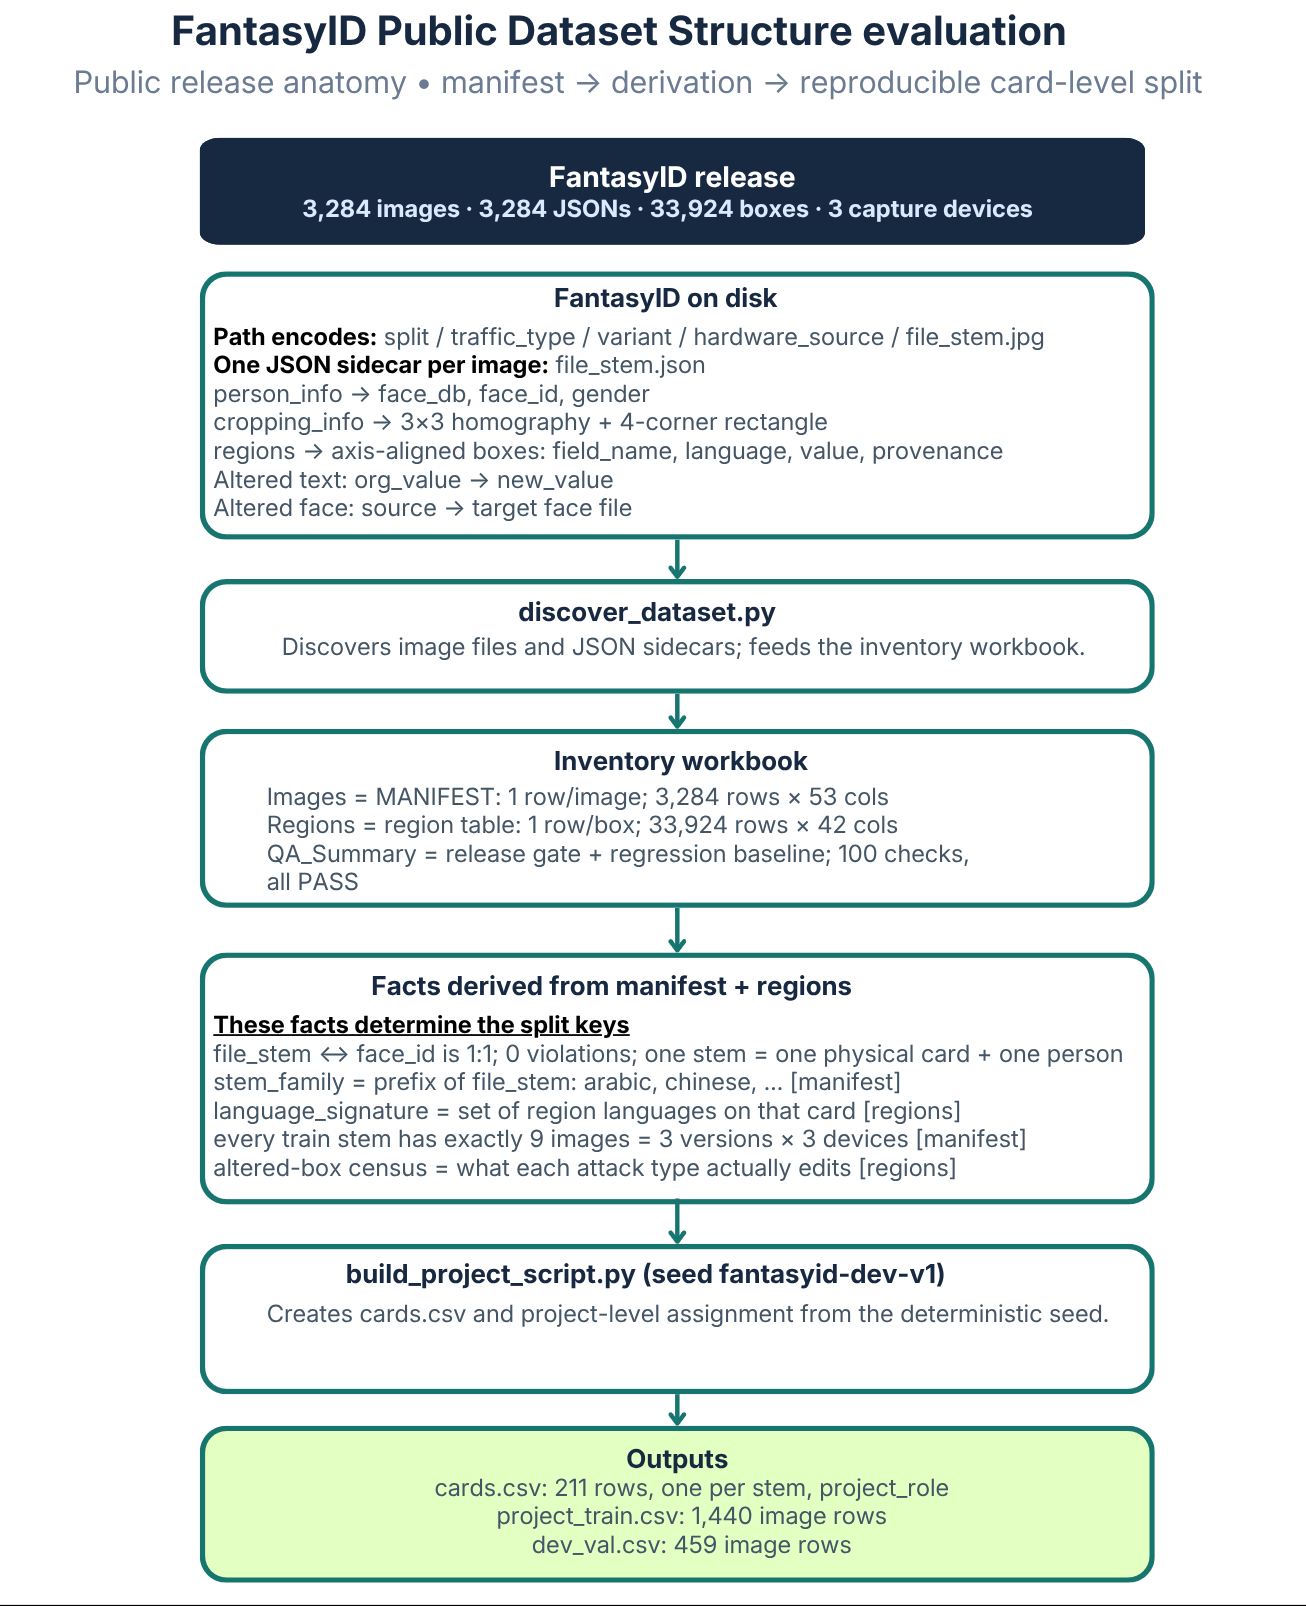
\includegraphics[width=0.95\textwidth,height=0.73\textheight,keepaspectratio]{Images/CH04_01.png}
\caption{Evaluation process of Fantasy ID dataset along with discovered information.}
\label{fig:FantasyIDdatasetEval}
\end{figure}

\begin{landscape}
\thispagestyle{empty}

\begin{figure}[H]
\centering
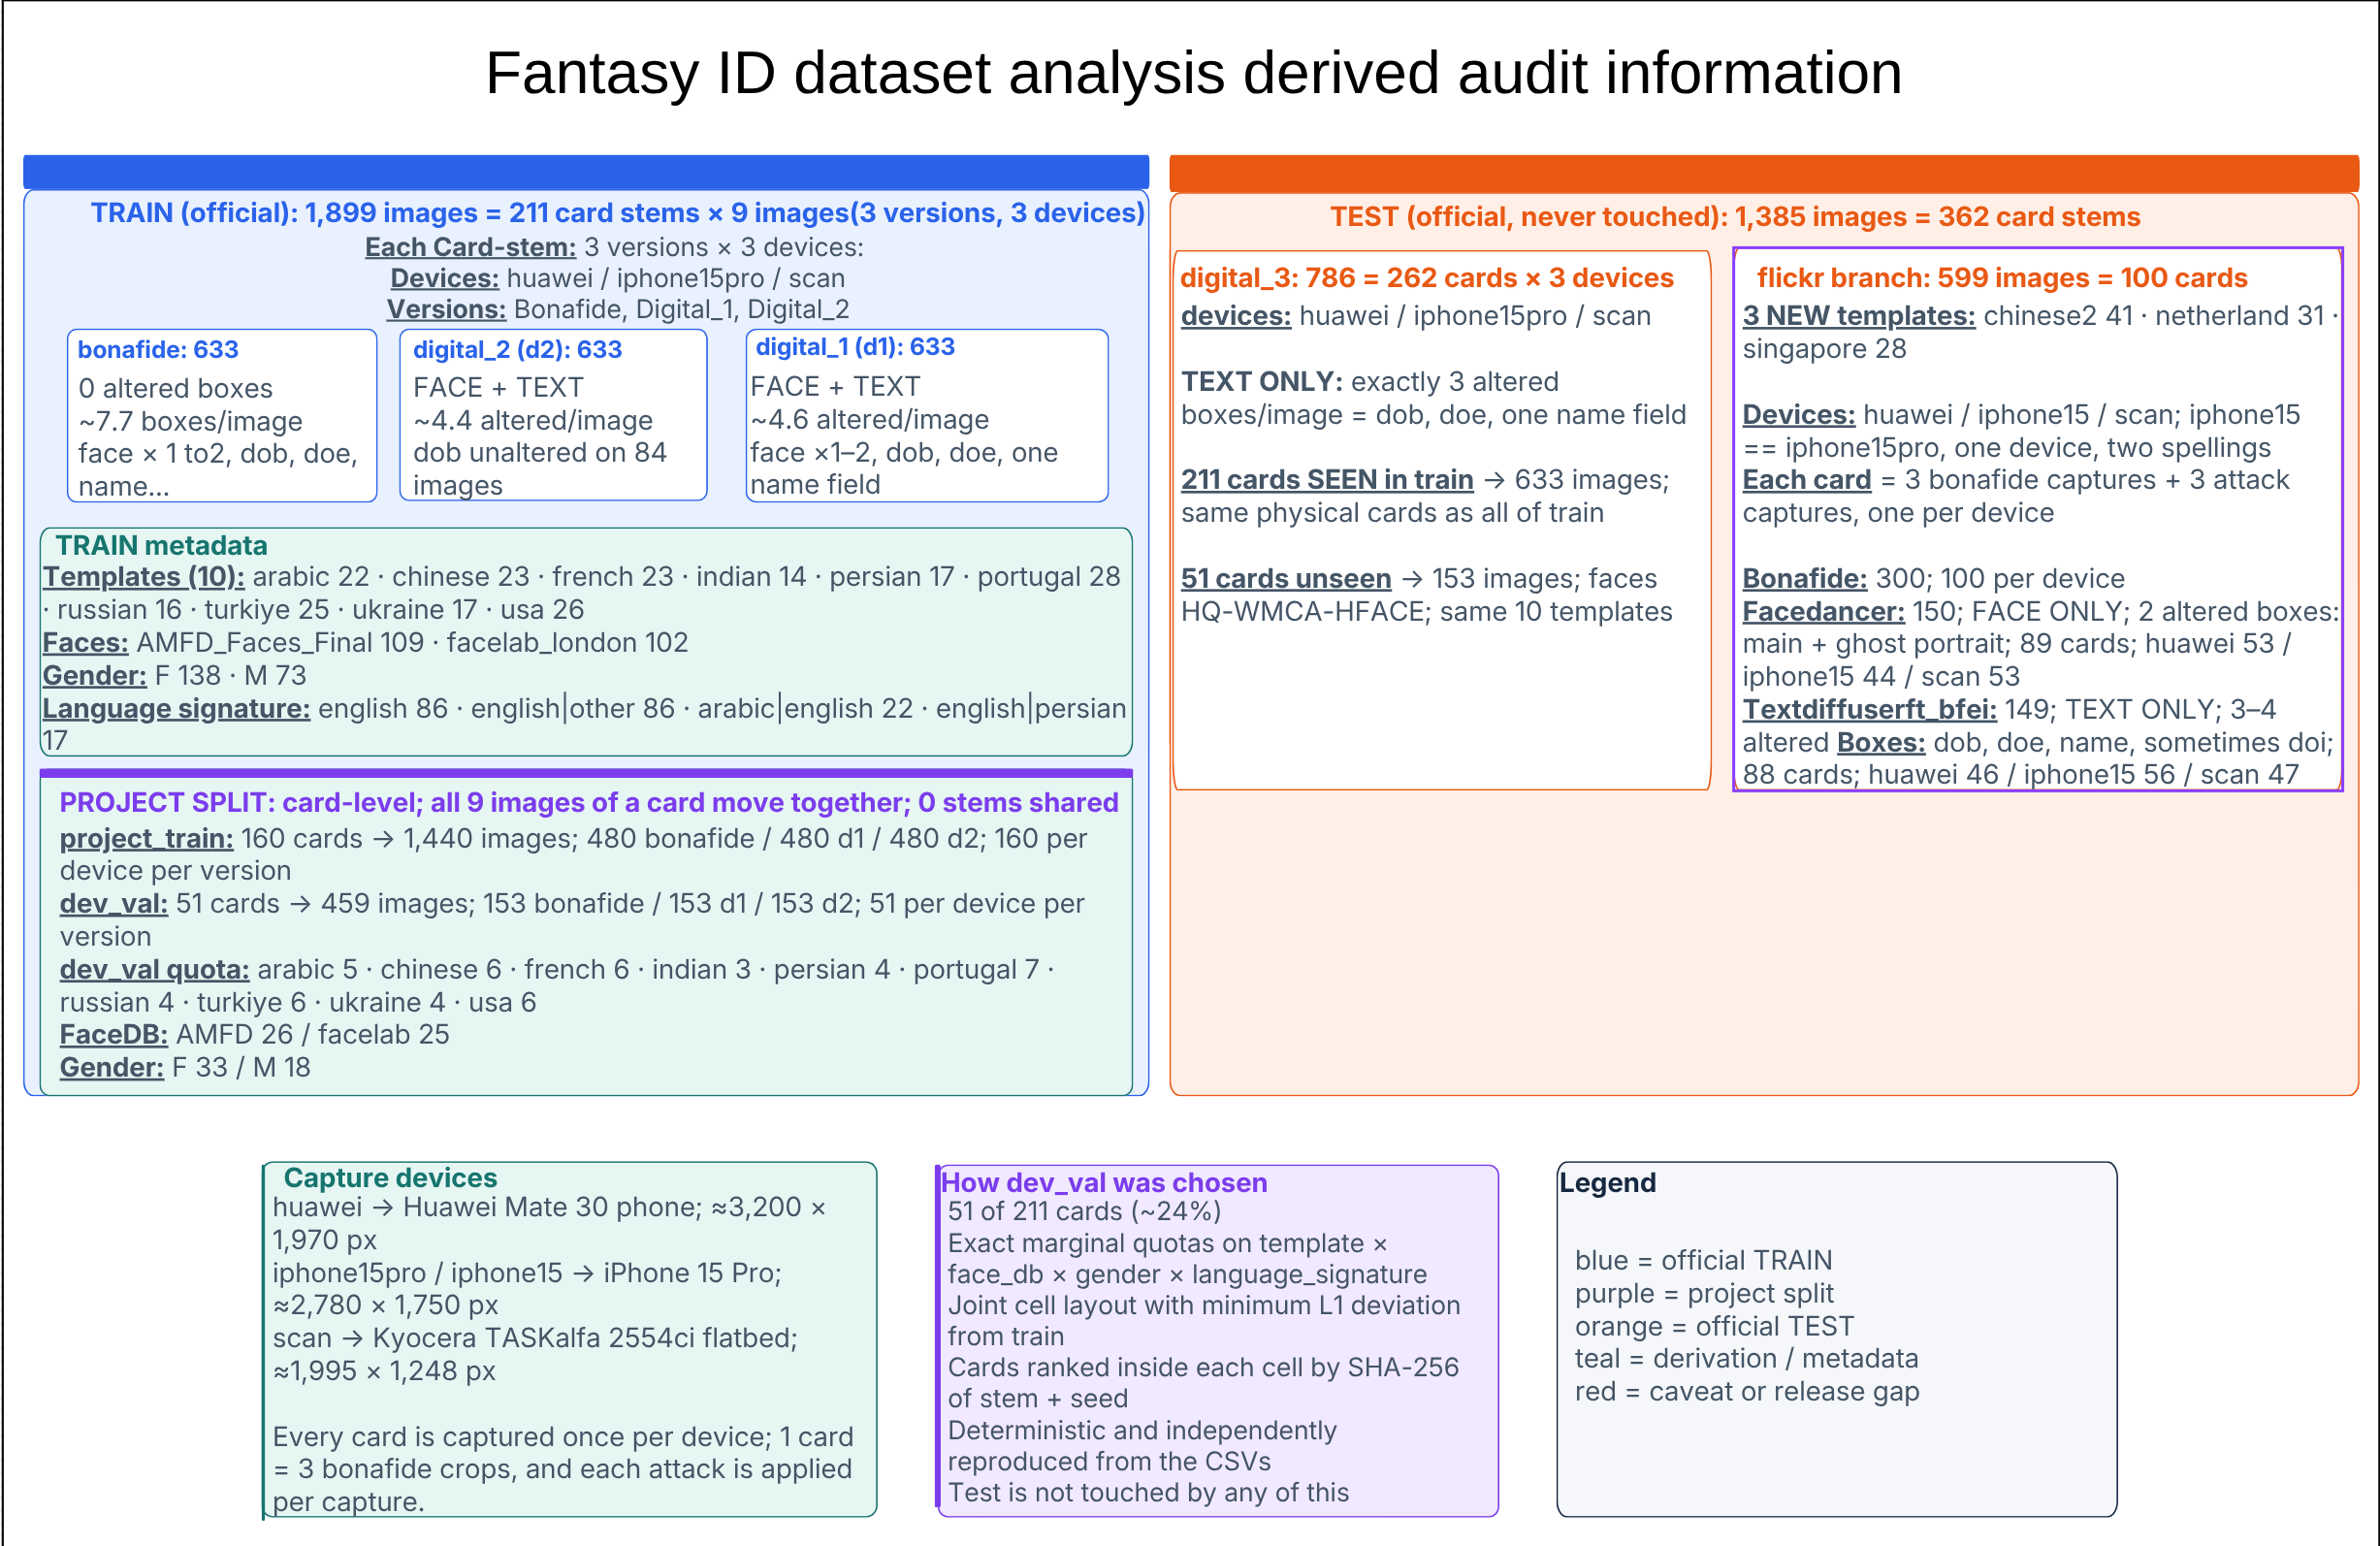
\includegraphics[
    width=1.0\linewidth,
    height=0.8\textheight,
    % keepaspectratio
]{Images/CH04_02_Dataset_Audit.png}
\caption{Fantasy ID dataset audit information.}
\label{fig:FantasyIDdatasetAudit}
\end{figure}

% Landscape page number
\begin{tikzpicture}[remember picture,overlay]
\node[rotate=90] at ([xshift=1.25cm]current page.west) {\thepage};
\end{tikzpicture}

\end{landscape}

ResNet-18 was trained on Digital-1 and Digital-2 categories and receives a resized document within a padded canvas. Grad-CAM is calculated from the forged-minus-bona-fide logit at the last residual block. TruFor keeps its pretrained weights, reads the document at its original resolution and produces a map of manipulation likelihood. Its \emph{decision} threshold was selected using the project-development images; its weights were not adapted in the final condition. ``Zero-shot'' therefore describes the weights, not an absence of calibration. 
%sa-review
% An earlier fine-tuning trial followed a different evaluation protocol and is recorded in Appendix~\ref{app:clean-trufor}, not merged with these results.

The development results are partly apparent performance: they informed ResNet checkpoint selection and TruFor threshold calibration. The official test prompted some later diagnostics, which are identified below as post-hoc checks. Training exposure, image resolution, map meaning and calibration all differ between pipelines. The main question remains how each pipeline's spatial output holds up against \emph{its own} clean baseline.

\section{Checking the compression shortcut}
\label{sec:clean-shortcut}

An initial audit found an alternative explanation for very good development detection. JPEG-history features alone separated forged from bona-fide development images with AUROC 1.000. The audit fitted a simple \emph{logistic-regression classifier} on compression features from project training, then tested it on the stem-disjoint development set. It showed that preparation history could reveal the class without examining the edited face or field. This is the kind of shortcut discussed in Chapter~2 \citep{geirhos2020shortcut}.

Policy C was adopted to reduce this class-correlated cue. Table~\ref{tab:clean-policy-c} gives the actual image sequence; the two JPEG encodings are separate, with a decode between them. The final quality is deterministic for a document stem and capture source, so its forged and bona-fide versions receive the same assignment. Chapter~3 and Appendix~\ref{app:clean-resnet} give the implementation and the reasons for choosing this policy.

\begin{table}[htbp]
\centering\small
\caption{Policy C at a glance. The same final quality is assigned to images from the same card and capture source. This is an outline of the implemented sequence, not a new image enhancement method.}
\label{tab:clean-policy-c}
\begin{tabularx}{\textwidth}{@{}lp{0.30\textwidth}X@{}}
\toprule
Step & Input and operation & Output \\
\midrule
1 & Decode the source JPEG to RGB. & Source pixels in memory. \\
2 & Encode those pixels as JPEG at quality 75, 4:2:0. & Common intermediate JPEG. \\
3 & Decode the intermediate JPEG to RGB. & Intermediate pixels in memory. \\
4 & Encode at a deterministic, matched quality from 50 to 90, 4:2:0. & Generates the Policy-C image used in evaluation. \\
\bottomrule
\end{tabularx}
\end{table}

Using the same kind of logistic-regression probe after this control,following was observed. 
\begin{itemize}
    \item Final JPEG-table features alone gave development AUROC 0.500.
    \item Broader JPEG-history features gave 0.524.
    \item All measured compression features together gave 0.586, with a stem-resampled 95\% interval [0.572, 0.606].
\end{itemize}
These are \emph{different feature sets}, not three scores for one unchanged input. The aim was to harmonise a preparation cue correlated with the class, not to remove every encoding trace a real edit might leave.

Both evaluated pipelines use Policy-C images. Recompression could weaken a useful forensic trace, while residual histories could still influence a decision. The results describe this controlled condition, not performance on the source files or in a bank. The regional intervention below, tests whether ResNet also responds to edited content under the control. It cannot restore traces lost through recompression or exclude every shortcut. These limits are retained in the Appendix~\ref{app:clean-resnet} risk register.

\section{Document decisions across forgery families}
\label{sec:clean-detection}

DeepID competition style overall reporting provides a useful first view: it includes false alarms on genuine cards as well as missed forgeries. Table~\ref{tab:clean-pooled} uses class-weighted F1, as in the competition's detection reporting, alongside accuracy, balanced accuracy and the underlying correct counts \citep{korshunov2025deepid}. These are \emph{this study's} Policy-C results at its chosen decision thresholds. They are not challenge leaderboard scores: the inputs and TruFor threshold differ from the challenge protocol, and the private competition set was not evaluated here. DeepID also scores binary localisation masks; the spatial measures later in this chapter answer a different question.

\begin{table}[htbp]
\centering
\small
\setlength{\tabcolsep}{4.5pt}
\caption{Pooled clean detection under this study's protocol. ``Forged DC(Decision-Correct)'' and ``BF(Bona-fide) correct'' give the numerators and denominators behind the summary. Accuracy, balanced accuracy (BA), class-weighted F1 and AUROC are calculated separately for each split.}
\label{tab:clean-pooled}

\begin{tabular}{@{}ll|cc|rrrr@{}}
\toprule
Split & Pipeline & Forged DC & BF correct & Accuracy & BA & Weighted F1 & AUROC \\
\midrule

Dev & ResNet-18 & 306/306 & 148/153 & .989 & .984 & .989 & 1.000 \\
Dev & TruFor & 288/306 & 73/153 & .786 & .709 & .769 & .843 \\
\midrule

Test & ResNet-18 & 182/1,085 & 209/300 & .282 & .432 & .274 & .234 \\
Test & TruFor & 1,042/1,085 & 131/300 & .847 & .699 & .831 & .944 \\

\bottomrule
\end{tabular}
\end{table}

An overall figure as noted in Table~\ref{tab:clean-pooled} and used in competitions cannot show \emph{which} kind of forgery a model detects or whether its spatial map points to the edit. Table~\ref{tab:clean-detection} therefore retains the family results. AUROC is the chance that a randomly selected forgery receives a higher forgery score than a randomly selected genuine document, across decision thresholds. Each family AUROC uses that family's forgeries and the bona-fide pool from the \emph{same split}. DC and balanced accuracy refer instead to the selected operating threshold. Balanced accuracy is $(\text{forged recall}+\text{bona-fide specificity})/2$; the same genuine pool is reused for each family in a split. 
%sa-review
% It should not be confused with the forged-only DC population used for spatial evidence.

\begin{table}[htbp]
\centering
\small
\setlength{\tabcolsep}{4.5pt}
\caption{Clean detection by forgery family. Forged $n$ is the original family size. DC is the number correctly called forged; BA includes genuine images from the same split. All results use the final fixed decision thresholds.}
\label{tab:clean-detection}

\begin{tabular}{@{}llr|rrr|rrr@{}}
\toprule
 & & &
\multicolumn{3}{|c}{ResNet-18} &
\multicolumn{3}{|c}{TruFor} \\
\midrule

Split & Family & Forged $n$
& AUROC & DC/$n$ & BA
& AUROC & DC/$n$ & BA \\
\midrule

Dev & Digital-1 & 153 & 1.000 & 153/153 & .984 & .986 & 153/153 & .739 \\
Dev & Digital-2 & 153 & 1.000 & 153/153 & .984 & .699 & 135/153 & .680 \\
\midrule

Test & Digital-3 & 786 & .059 & 6/786 & .352 & .999 & 786/786 & .718 \\
Test & FaceDancer & 150 & .958 & 144/150 & .828 & .601 & 107/150 & .575 \\
Test & TextDiffuserFT & 149 & .429 & 32/149 & .456 & .999 & 149/149 & .718 \\

\bottomrule
\end{tabular}
\end{table}

ResNet's 6/786 Digital-3 decisions and 32/149 TextDiffuser decisions reveal a much narrower test population for later evidence analysis than the pooled number suggests. 
TruFor detects every Digital-3 and TextDiffuser image here, but at its fixed threshold it also flags 169 of the 300 genuine test cards. 

High AUROC on those families describes score ranking however it does not undo the false-positive rate. The large Digital-3 family can also dominate a pooled score while a smaller family behaves differently.

ResNet uses a forged-score threshold of 0.5. TruFor uses one threshold, 0.532956, selected on development images for every family and capture source. 
%sa-review
% These classification thresholds are distinct from the two, still-unfrozen requirements for acceptable spatial evidence. Table~\ref{tab:clean-trufor-threshold} shows the trade-off against TruFor's upstream 0.5 operating point. The selected threshold improved apparent development accuracy and genuine specificity but missed five more forgeries. It was fitted to equal-weight image accuracy on these development images, not to a bank's cost of accusing a genuine customer.
These classification thresholds are distinct from the requirements for acceptable spatial evidence. Table~\ref{tab:clean-trufor-threshold} shows the trade-off against TruFor's upstream 0.5 operating point. The selected threshold improved apparent development accuracy and genuine specificity but missed five more forgeries. It was fitted to equal-weight image accuracy on these development images, not to a bank's cost of accusing a genuine customer.

\begin{table}[htbp]
\centering
\small
\setlength{\tabcolsep}{5pt}
\caption{TruFor development decisions at two fixed thresholds. The selected threshold was fitted on these same 459 images; the table is a calibration diagnostic, not independent validation. AUROC is unchanged because the score order does not change.}
\label{tab:clean-trufor-threshold}

\begin{tabular}{@{}l|cc|rrr@{}}
\toprule
Forged-score threshold & Forged DC & BF correct & Accuracy & BA & Weighted F1 \\
\midrule

Upstream .500 & 293/306 & 51/153 & .749 & .645 & .714 \\
Selected .532956 & 288/306 & 73/153 & .786 & .709 & .769 \\

\bottomrule
\end{tabular}
\end{table}

The one TruFor threshold also behaves unevenly across development capture sources (Table~\ref{tab:clean-trufor-device}). For Huawei captures, only five of 51 genuine cards are accepted; the corresponding number for iPhone15Pro is 41 of 51. The groups are small and related through card identities. No device-specific threshold was fitted after seeing this spread.

\begin{table}[htbp]
\centering\small
\caption{TruFor development results by capture source at the single selected threshold. Source-specific BA uses only that source's forged and bona-fide images; each group contains 102 forgeries and 51 genuine cards.}
\label{tab:clean-trufor-device}

\begin{tabular}{@{}l|cc|cc@{}}
\toprule
Capture source & Forged DC & BF correct & BF specificity & BA \\
\midrule
Huawei & 99/102 & 5/51 & 9.8\% & .534 \\
iPhone15Pro & 96/102 & 41/51 & 80.4\% & .873 \\
Scan & 93/102 & 27/51 & 52.9\% & .721 \\
\bottomrule
\end{tabular}
\end{table}

\section{Does ResNet respond to the edited regions?}
\label{sec:clean-regions}

For ResNet, the development score were near perfect but test scores did not match up to that. Further, the development forgeries contain altered face and text regions, whereas the unseen families in test dataset change the mix of manipulations. The uneven decisions above raised a practical question of whether ResNet-18 learnt cues from both kinds of region edits(face, text), or mainly from one? 
A larger face edit might be easier for a whole-document classifier to learn than a small text change, but that is a hypothesis, not an explanation supplied by the detection scores. Hence the regional test was designed to examine that possibility.

% Optional explanatory image to add when its annotation and edit-family
% descriptions have been checked against the actual FantasyID family records.
% Suggested file: Images/CH04_Family_Edit_Contrast_V1.pdf.
%sa-review
\IfFileExists{Images/CH04_Family_Edit_Contrast_V1.pdf}{%
\begin{figure}[htbp]
\centering
\includegraphics[width=0.94\textwidth]{Images/CH04_Family_Edit_Contrast_V1.pdf}
\caption{Illustrative face and text annotations in the development families and examples from unseen test families. The panels illustrate edit scale; they are not a measurement of why a classifier succeeds or fails.}
\label{fig:clean-family-edits}
\end{figure}
}{}

For each suitable development image, the annotated face or text was replaced with the corresponding region from the same card's bona-fide capture. Geometry and JPEG processing were matched. Figure~\ref{fig:clean-restoration} reports the average of ResNet's forged-class scores \emph{over the same paired cards} before and after replacement. This shows score movement even when both scores lead to the same class decision; it is neither a localisation score nor a calibrated probability of fraud.

\begin{figure}[htbp]
\centering
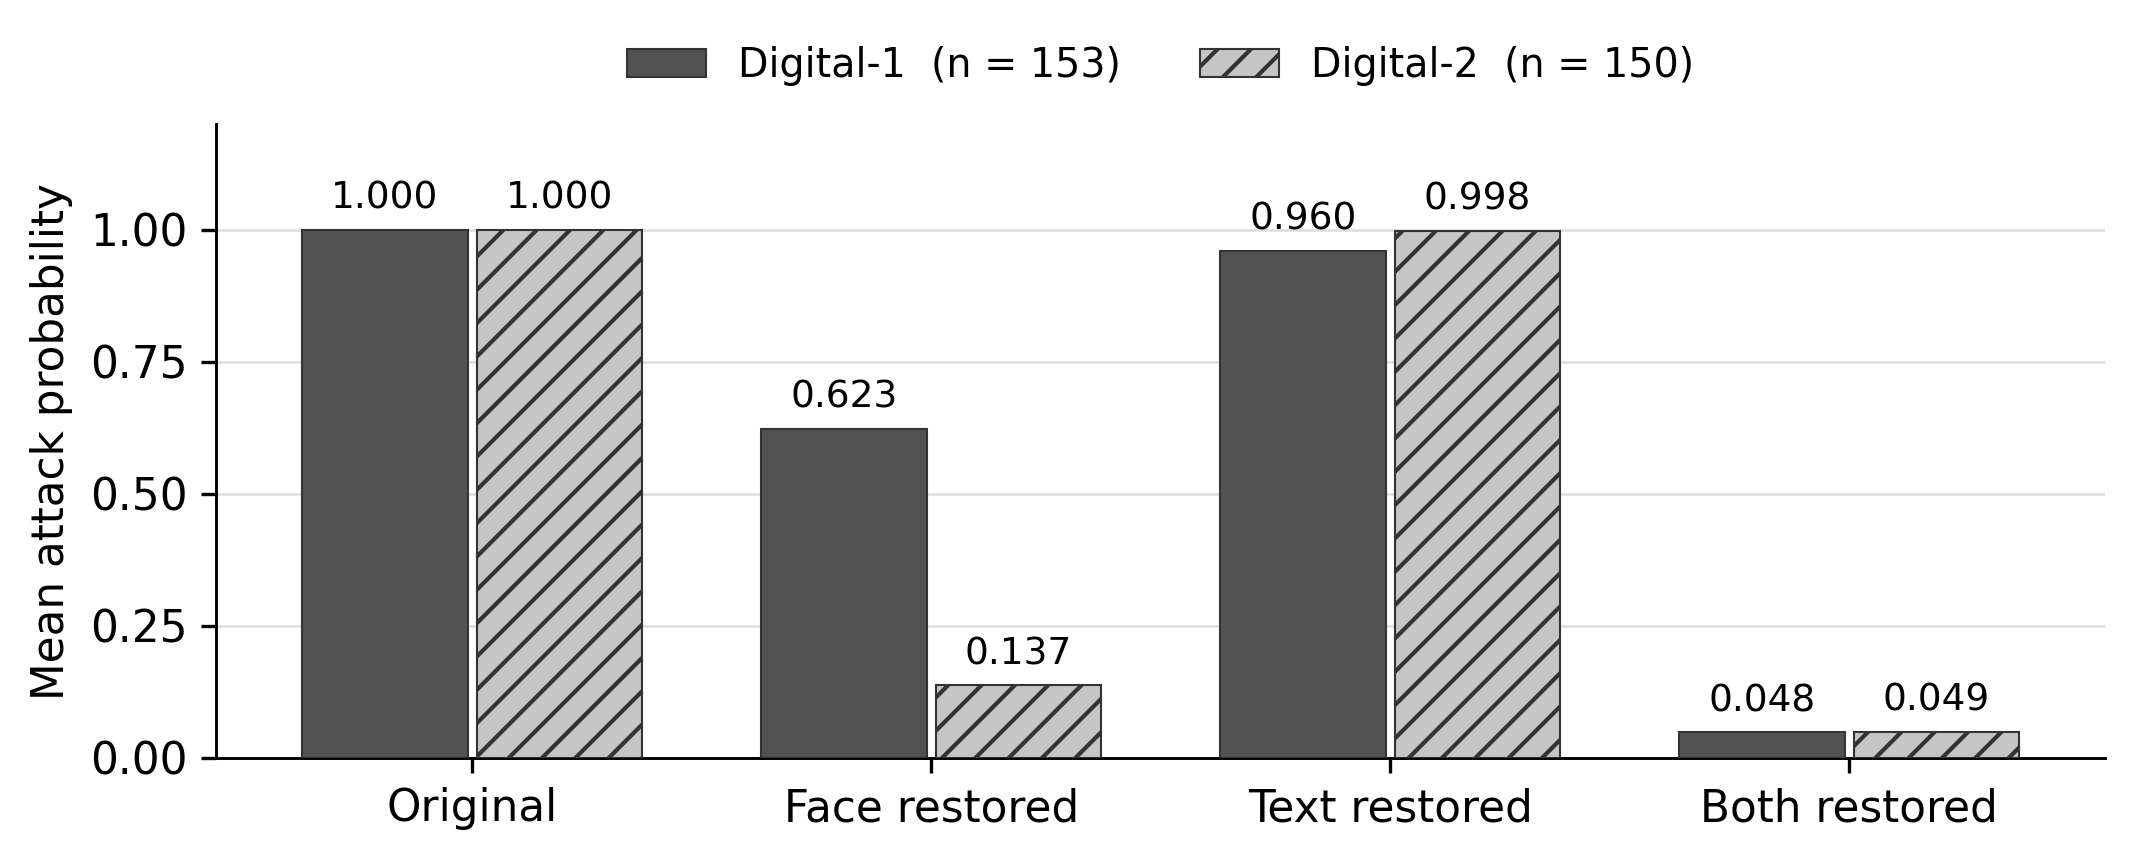
\includegraphics[width=0.96\textwidth]{Images/CH04_Restoration_V1.png}
\caption{Mean ResNet forged-class scores after same-card regional restoration on development images. Digital-1 uses 153 pairs; Digital-2 uses 150 because three pairs have incompatible geometry. Bars describe paired image-score averages, not the effect of a single isolated forensic feature.}
\label{fig:clean-restoration}
\end{figure}

On Digital-2 from development dataset, the mean score falls from almost 1.000 to 0.137 when the face is restored, but remains 0.998 when only text is restored. Restoring both regions brings it near the genuine-card score of 0.049. This supports stronger dependence on face-region content under the tested intervention. 

It does not prove that text never matters or reveal the exact texture used. Replacement can also change local boundaries. Although the procedure matches JPEG processing and geometry, a separate classifier test of post-restoration artifacts was also performed. Its results evidence that post-restoration artifacts were not enough to separate out post-restoration artifacts.
%sa-review
Altered boundaries still remain a residual risk in Appendix~\ref{app:clean-resnet}. A restoration-augmented training trial improved some internal cue balance but left official-test AUROC at 0.089 for Digital-3 and 0.463 for TextDiffuser. It was a diagnostic, not the primary model regardless.

Digital-3 from test dataset required another check. In 153 pairs, an \emph{official-test Digital-3 forgery} was matched to the bona-fide parent card in this project's development data. The forgery's score rose relative to its own parent in 82.4\% of pairs. Yet the average increase was only 0.0094 and its stem-resampled interval included zero; the same-source AUROC was 0.628 [0.592, 0.669]. The official-test AUROC of 0.059 instead compares all 786 Digital-3 forgeries with a different pool of 300 official-test bona-fide cards. These checks suggest that a weak response to the edit and a change in the comparison population could both matter. They do not identify a single proven cause, and the paired check was pursued after the official-test result was seen purely as diagnostics.

\section{Agreement between maps and altered regions}
\label{sec:clean-spatial}

Chapter~2 introduced altered-area fraction $A$ (Area) and $E$ as the Relevance Mass Accuracy (RMA). $E$ is the fraction of map mass inside the annotated region; $A$ is the fraction of valid document area it occupies. The ratio $\mu_w=E/A$ expresses how concentrated the map is relative to that area's size. If a map spreads its mass evenly, $E$ is close to $A$. 

The Pointing Game (PG) asks only whether the \emph{single strongest} map pixel falls inside an annotated region. Relevance rank accuracy (RRA) checks how many of the strongest pixels, selected in the same number as the altered pixels, lie inside it. Appendix~\ref{app:clean-metrics} specifies the per-image calculations and invalid-map rules.

Table~\ref{tab:clean-spatial} keeps three denominators visible: the original forged family, its clean DC subset and the maps evaluated. All displayed map summaries are now restricted to DC. In particular, the archived ResNet FaceDancer audit covered all 150 maps; this table filters its individual-image records to the 144 correctly detected images, so its means differ slightly from the earlier whole-family description. ResNet excludes its artificial padding when calculating map agreement. TruFor uses its native manipulation map. 
%sa-review??????????????????????????????
A common-coordinate RRA audit still needs to be completed before setting the final evidence gate.

\begin{table}[htbp]
\centering\small\setlength{\tabcolsep}{5pt}
\caption{Clean spatial agreement, conditional on a correct forgery decision. ``All'' is the original family size, ``DC'' the correctly detected count and ``maps'' the number summarised. $A$ is altered document area in percent; $E$ and PG are fractions. The displayed $\mu_w$ is the mean of per-image $E_i/A_i$, not the ratio of the displayed means. ResNet's FaceDancer row is calculated from its per-image records after filtering to DC.}
\label{tab:clean-spatial}
\begin{tabular}{@{}llr|rr|r|rrr@{}}
\toprule
Map & Family & All $n$ & DC $n$ & Maps $n$ & $A$ (\%) & $E$ & $\mu_w$ & PG \\
\midrule
Grad-CAM & Digital-1 (dev) & 153 & 153 & 153 & 15.9 & .707 & 4.77 & 1.000 \\
Grad-CAM & Digital-2 (dev) & 153 & 153 & 153 & 9.3 & .546 & 6.16 & .523 \\
\midrule
Grad-CAM & Digital-3 (test) & 786 & 6 & 6 & 2.6 & .0007 & .03 & .000 \\
Grad-CAM & FaceDancer (test) & 150 & 144 & 144 & 6.6 & .494 & 7.82 & .722 \\
Grad-CAM & TextDiffuserFT (test) & 149 & 32 & 32 & 4.3 & .010 & .24 & .000 \\
\midrule
\addlinespace

TruFor & Digital-1 (dev) & 153 & 153 & 153 & 15.7 & .555 & 3.90 & 1.000 \\
TruFor & Digital-2 (dev) & 153 & 135 & 135 & 9.3 & .192 & 2.09 & .504 \\
\midrule
TruFor & Digital-3 (test) & 786 & 786 & 786 & 2.9 & .642 & 23.26 & .991 \\
TruFor & FaceDancer (test) & 150 & 107 & 107 & 6.9 & .112 & 1.70 & .402 \\
TruFor & TextDiffuserFT (test) & 149 & 149 & 149 & 4.2 & .703 & 17.13 & 1.000 \\
\bottomrule
\end{tabular}
\end{table}

The ``means'' help describe a family, but can hide how varied its individual maps are. Table~\ref{tab:clean-spatial-median} gives the median and middle half of the image-level $E$ values behind the preceding table. These are descriptive distributions for DC images, not DCEC pass rates.

\begin{table}[htbp]
\centering\small
\caption{Median relevance mass $E$ and interquartile range (IQR) among the DC images in Table~\ref{tab:clean-spatial}. Values are computed from per-image map records; RRA thresholds are not inferred from this table.}
\label{tab:clean-spatial-median}
\begin{tabular}{@{}ll|c|c@{}}
\toprule
Map & Family & Median $E$ & $E$ IQR \\
\midrule
Grad-CAM & Digital-1 (dev) & .708 & [.639, .784] \\
Grad-CAM & Digital-2 (dev) & .520 & [.467, .624] \\
Grad-CAM & Digital-3 (test) & .00032 & [.00005, .00150] \\
Grad-CAM & FaceDancer (test) & .531 & [.367, .581] \\
Grad-CAM & TextDiffuserFT (test) & .00266 & [.00031, .01199] \\
\addlinespace
TruFor & Digital-1 (dev) & .550 & [.406, .693] \\
TruFor & Digital-2 (dev) & .157 & [.112, .232] \\
TruFor & Digital-3 (test) & .697 & [.453, .859] \\
TruFor & FaceDancer (test) & .102 & [.084, .124] \\
TruFor & TextDiffuserFT (test) & .778 & [.579, .860] \\
\bottomrule
\end{tabular}
\end{table}

\newpage
%sa-review add image!!!!
An ID can have both a changed face and changed text. A high $E$ over the \emph{combined} annotation could still come entirely from the face. A PG success only establishes that one peak falls somewhere inside that combined area. Table~\ref{tab:clean-components} therefore separates the face and text contributions on the two development families. For Digital-2, ResNet places an average 0.540 of its total map mass in the face region but only 0.006 in text, even though its union $E$ is 0.546. Its strongest point is in the combined annotation in only 80 of 153 cases. The component results expose what the union summary misses.

\begin{table}[htbp]
\centering\small
\caption{Mean share of total map mass in the annotated face and text regions on correctly detected development forgeries. The union is the existing $E$ measure; component results are shown because a union-level score need not cover both edits. Face and text annotations can overlap, so their shares need not add exactly to the union.}
\label{tab:clean-components}
\begin{tabular}{@{}llr|rrr@{}}
\toprule
Map & Dev family & DC maps $n$ & Face $E$ & Text $E$ & Union $E$ \\
\midrule
Grad-CAM & Digital-1 & 153 & .658 & .049 & .707 \\
Grad-CAM & Digital-2 & 153 & .540 & .006 & .546 \\
\midrule
TruFor & Digital-1 & 153 & .359 & .197 & .555 \\
TruFor & Digital-2 & 135 & .161 & .031 & .192 \\
\bottomrule
\end{tabular}
\end{table}

ResNet's FaceDancer maps (test) show meaningful concentration on the edited area when restricted to the 144 DC images; its six correctly detected Digital-3 maps (test) and 32 TextDiffuser maps (test) show very little. Six Digital-3 examples cannot represent that 786-image family. 

TruFor gives stronger clean spatial agreement on Digital-3 and TextDiffuser but weaker agreement on FaceDancer. 

These differences describe the \emph{implemented pipelines}, with different outputs and resolutions. The attack question compares each one to its own starting maps, so no claim that one architecture is inherently better is needed.

For the \emph{mean $E$} values in Table~\ref{tab:clean-spatial}, ResNet's Digital-1 and Digital-2 development rows have document-stem-resampled 95\% intervals [0.677, 0.736] and [0.513, 0.578], respectively. They describe sampling variation across these document stems for this fitted model. They do not include a new training seed or uncertainty in the annotation rectangles. Neither means nor medians can tell us how many individual maps pass both eventual $E$ and RRA requirements.

\section{Visual review and the unfinished evidence gate}
\label{sec:clean-review}

The supplied rectangles approximate a manipulation, and an enlarged Grad-CAM map is coarse. A visual check is therefore needed alongside numeric agreement. The author is reviewing development maps against the altered document and its same-card bona-fide reference. Face and text are rated separately, with an ambiguous category where a yes/no judgement would overstate what can be seen. The ongoing coding task uses the displayed images and maps rather than per-image $E$, RRA, proposed DCEC membership or attack outcomes. Appendix~\ref{app:clean-metrics} gives the coding sheet, sampling procedure and intended threshold-selection rule.

This is an \emph{author-conducted contextual review}. The author has seen some aggregate results before rating the images, so it cannot be presented as an independent or prospectively blind assessment. Consistent display rules and a repeat rating of selected images can help expose inconsistent judgements; they cannot turn those judgements into ground truth or show how a document examiner would use a map. Ratings, agreement statistics and the final joint $E$/RRA thresholds remain incomplete at this version.

The order of work must also be disclosed. Attacks were first run on the broader DC population, before the clean-evidence rule was finalised. The remaining control is to choose the evidence rule from clean development measurements and the declared visual ratings, without optimising it against attack success. Official-test results, attack outcomes and a convenient eligible sample size must not select the thresholds. Prior analyst exposure remains a limitation. Appendix~\ref{app:clean-metrics} records the sensitivity checks needed before a DCEC claim, including coordinate conventions, uncertain rectangle boundaries and component coverage.

\section{What the clean population supports}
\label{sec:clean-populations}

Across the five manipulated families, ResNet has 488 observed DC images and TruFor has 1,330. These totals combine the development and official-test family counts in Table~\ref{tab:clean-detection}; they are \emph{not} evidence-eligible sample sizes. For each pipeline, the eventual DCEC gate will retain DC images whose clean $E$ and RRA both meet its accepted thresholds. The same accepted thresholds must then be used on that pipeline's attacked maps. Until calibration and coordinate checks finish, no DCEC coverage or shared-DCEC intersection can be reported.

The full denominator trail is original forged family $\rightarrow$ clean DC $\rightarrow$ clean DCEC. Low coverage at any stage will be reported, not hidden by reporting success only among eligible examples. Within the fixed DCEC set, DCEW means the attack makes spatial evidence fail while the forgery decision stays correct. A classification flip remains in the original DCEC denominator but is reported separately. The existing attacks on DC images can be analysed again under the later clean-only eligibility rule without rerunning them. Images eligible for both pipelines may provide matched visual examples and another view of \emph{within-pipeline} degradation; their intersection is not a controlled architecture comparison.

\section{Conclusion}
\label{sec:clean-conclusion}

The clean audit shows why a correct document decision is only a first step. ResNet's very strong development detection does not carry evenly to unseen forgery families, and its Digital-2 map is concentrated mainly on the face. TruFor has different strengths across families and many false alarms on genuine official-test cards at its selected threshold. The compression and regional checks narrow some alternative explanations while leaving documented risks. Objective O1 now has a clear detection and continuous spatial baseline; O2's author review and joint evidence calibration are still under way. Chapter~5 will assess adversarial evidence degradation against each pipeline's fixed clean DCEC population once that population is established.

% Chapter 5, version 1 (05V1.tex), 23 September 2026.
% Requires amsmath, graphicx, booktabs, tabularx, array and natbib.
% Companion scientific figure: Images/CH05_ResNet_LossDistribution_V1.pdf.
% Insert as Chapter 5 before the appendix sequence. The companion
% 05_AppendixV1.tex occupies Appendix E; Appendix D is reserved.
% IMPORTANT: No numeric DCEC-to-DCEW rate can yet be stated. The joint
% E/RRA clean gate and paired RRA evaluation are still unfinished.

\chapter{Adversarial Evaluation of Spatial Evidence}
\label{ch:adversarial}

\section{What is being tested}
\label{sec:adv-question}

Chapter~\ref{ch:clean} established that a correct forgery decision does not always come with a useful map. This chapter examines a different failure: whether a small, deliberate change to an image can make its map agree less with the annotated alteration while the detector still calls the image forged. The perturbation is applied \emph{after} the forgery and after the controlled JPEG preparation. It does not repair or move the alteration.

The analysis begins with DC, the forged images that each pipeline called correctly before the extra perturbation. On these images, the paired change in relevance mass $E$ measures how much of the map falls inside the annotated region before and after the attack. The stricter outcome in the research question starts with DCEC: images that also have acceptable \emph{clean} spatial evidence under the joint $E$/RRA rule. An image becomes DCEW only when it was in that fixed DCEC set, its forged decision remains correct, and its adversarial $E$ \emph{or} RRA falls below the original evidence threshold. A classification flip is a separate outcome and stays in the DCEC denominator. Appendix~\ref{app:adv-details} gives the recording rules.

The full ResNet-18/Grad-CAM attacks have been run on 450 DC images. They give a substantial paired result for $E$ and a useful classification-attack control. TruFor's attack settings have been frozen and its full run is in progress; an exact native-resolution gradient route and a one-image attack check have been completed. The clean human review, joint $E$/RRA thresholds and paired RRA results still need to be completed for both pipelines. For that reason, this chapter reports the measured DC results and leaves visible markers for the final DCEC-to-DCEW rates. It does not turn a fall in mean $E$ into an unmeasured binary success rate.

The attacks are white-box: they use the model's gradients and the altered-region annotations to seek a low $E$. This tests what is possible under a deliberately informed attacker. It is stronger access than a typical document submitter would have; the results concern these evaluated pipelines, not an observed attack on a live verification service. Work on explanation attacks shows why holding the label fixed matters, while document-localisation attacks provide a related, but different, forensic precedent \citep{ghorbani2019fragile,dombrowski2019explanations,shao2025documentrobustness}. Here loss of \emph{annotation agreement}, rather than mere visual difference between maps, is the measured outcome.

\section{Attack population and controls}
\label{sec:adv-population}

Table~\ref{tab:adv-populations} starts from the clean decisions reported in Chapter~\ref{ch:clean}. Each family is counted separately. ResNet's primary attack families were chosen after the clean audit: Digital-1, Digital-2 and FaceDancer had enough correct decisions and interpretable clean map agreement to examine degradation. Digital-3 had only 6/786 correct ResNet forgery decisions and near-zero clean $E$; TextDiffuserFT had 32/149 correct decisions and mean $E=0.010$ on those DC images. Calling further loss of their already poor evidence an adversarial explanation failure would obscure the more basic clean failure. This selection limits coverage and must remain visible alongside the attack result.

TruFor's DC population is larger, but DC does not tell us how many maps will pass the eventual joint evidence rule. Its weak clean Digital-2 and FaceDancer map agreement is a particular reason to retain DCEC coverage by family. The two models operate at their previously selected decision thresholds: attack probability $0.5$ for ResNet and forged score $0.532956$ for TruFor. These thresholds remain fixed after seeing attack outcomes. Their image sizes, training exposure and map types also differ, so the main comparison is an attacked image against its \emph{own pipeline's} clean map, not an unqualified contest between models.

\begin{table}[htbp]
\centering\small
\caption{Forged images entering the adversarial analysis. DC counts are clean, correct decisions; they do not establish DCEC eligibility. ResNet's primary decision-preserving attack covers its three indicated families.}
\label{tab:adv-populations}
\begin{tabular}{@{}llrrl@{}}
\toprule
Split & Forgery family & Total & ResNet DC & TruFor DC \\
\midrule
Dev & Digital-1 & 153 & 153 & 153 \\
Dev & Digital-2 & 153 & 153 & 135 \\
Test & Digital-3 & 786 & 6 & 786 \\
Test & FaceDancer & 150 & 144 & 107 \\
Test & TextDiffuserFT & 149 & 32 & 149 \\
\midrule
 & DC roster for evidence attack & & $450^{\dagger}$ & $1{,}330^{\ddagger}$ \\
\bottomrule
\end{tabular}

\vspace{2pt}\parbox{\linewidth}{\footnotesize $^{\dagger}$Digital-1, Digital-2 and FaceDancer, completed. $^{\ddagger}$Frozen TruFor run roster across all five families; full population outcomes pending.}
\end{table}

Across these development and test splits there are 1,391 forged images. ResNet called 488 of them correctly, but its primary evidence attack covers 450, or 32.4\% of all 1,391. This is partly a consequence of poor clean detection on Digital-3 and TextDiffuserFT, not an adversarial exclusion chosen after seeing their attacked maps. TruFor's 1,330 clean-correct cases cover 95.6\% of all forgeries, although many may still have weak clean spatial evidence. These figures are useful coverage checks, not a like-for-like robustness score. Two ResNet attacked families are development families used in model selection; FaceDancer supplies the selected pipeline's principal unseen-family attack result.

Both evidence-directed attacks minimise $E$ within the union of the annotated altered regions while requiring the forged decision to remain correct. They use the same bound on changes to the RGB image, $\lVert\delta\rVert_\infty\leq1/255$ in $[0,1]$ units. Ten proposed gradient steps use a step size of $0.25/255$ and an eight-step feasibility pull-back when a proposal would cross the decision boundary. The attacks begin at the clean input without restarts. The unchanged Policy-C image is the baseline; no new crop or JPEG stage is applied during attack evaluation. For ResNet, only resized document-content pixels can change: its artificial side padding stays fixed. TruFor uses its full native-resolution document without padding. The precise model-space conversions and acceptance rules are in Appendix~\ref{app:adv-details}; an $L_\infty$ bound alone is not a perceptual study.

The ResNet classification-targeted PGD control asks a separate question: can a small perturbation change the \emph{decision} to bona fide? Its result is necessary for interpreting Grad-CAM. When the attack-class decision disappears, a heatmap calculated for that class may also disappear; that cannot be counted as a decision-preserving spatial-evidence failure. This distinction follows the evaluation caution in \citet{carlini2019evaluating}: the attack and success condition must match the property being claimed.

\section{ResNet: the classification-attack control}
\label{sec:adv-resnet-control}

The classification control evaluated 456 images at the $1/255$ bound: 153 Digital-1, 153 Digital-2 and all 150 FaceDancer images. It pushed the score toward bona fide with ten projected steps and a random start. Among the 450 initially correct decisions, all 153 Digital-1, 153 Digital-2 and 144 FaceDancer decisions flipped. The six other FaceDancer images were already misclassified and are excluded from the conditional flip rate and the paired map-loss figures below.

Grad-CAM's $E$ also fell among these clean-correct images: the mean per-image relative losses were 66.75\%, 97.72\% and 86.70\%, respectively. Yet the manipulated-class CAM had effectively zero positive mass on 30.7\% of Digital-1, 96.7\% of Digital-2 and 86.1\% of FaceDancer adversarial images. The evaluator records $E=0$ for such maps. It would be misleading to interpret those low $E$ values as evidence being directed toward the wrong part of a forged document: the forged classification was gone, and in many cases its positive map was gone too.

Three 72-image PGD pilots at $4/255$, $2/255$ and $1/255$ each flipped all 70 images that were initially correct; two FaceDancer cases were already wrong. The full control then used the smallest of these \emph{tested} conventional intensity-level budgets. No finer budget was tested, so the data do not locate a minimum perturbation at which decisions start to fail. They do show why the main evidence attack must enforce the original decision and check that its map remains defined.

This control has a practical implication for how the results should be read. At the tested bound, a white-box attacker targeting these selected ResNet images could simply seek a wrong forgery decision. The evidence-directed attack asks what can happen when the decision is \emph{held} correct and a person might still inspect its map. Neither result says how often an uninformed submitter could achieve that condition or whether a downstream system would accept the altered file.

\section{ResNet: reducing evidence while preserving the decision}
\label{sec:adv-resnet-evidence}

The evidence-directed ResNet attack differentiates through Grad-CAM and seeks to move map mass away from the annotated union. It maintains the forged-minus-bona-fide logit margin at or above zero and only accepts a feasible proposal if $E$ does not increase beyond a small numerical tolerance. The same frozen evaluator measured clean and adversarial maps after attack. All 450 final outputs stayed on the forged side of the decision threshold, all had nonzero positive CAM mass, and all 450 had strictly lower final $E$ than their corresponding clean images. That last observation is an evaluated end result; the optimisation rule does not demand strict improvement at \emph{every} accepted step.

Table~\ref{tab:adv-resnet-e} reports the most recent full visual rerun, consistently for all three families. The table pairs exactly the DC images that entered the attack. Its FaceDancer clean $E=0.4940$ therefore differs from Chapter~\ref{ch:clean}'s all-150 mean of $0.4888$. The column headed ``relative loss'' is the mean of each image's $100(E_{\rm clean}-E_{\rm adv})/E_{\rm clean}$, not the percentage formed by dividing the two displayed family means.

\begin{table}[htbp]
\centering\small
\caption{Completed ResNet decision-preserving attack on paired DC images. $E$ and PG are clean$\rightarrow$adversarial; relative loss averages image-wise losses. All attacked decisions remained forged and all adversarial CAMs were nonzero.}
\label{tab:adv-resnet-e}
\begin{tabular}{@{}lrrrrl@{}}
\toprule
Family & DC $n$ & Mean $E_{\rm clean}$ & Mean $E_{\rm adv}$ & Relative loss & PG, clean$\rightarrow$adv \\
\midrule
Digital-1 & 153 & .7066 & .1458 & 79.24\% & 1.000$\rightarrow$.673 \\
Digital-2 & 153 & .5460 & .1004 & 81.22\% & .523$\rightarrow$.235 \\
FaceDancer & 144 & .4940 & .0226 & 95.12\% & .722$\rightarrow$.000 \\
\bottomrule
\end{tabular}
\end{table}

Stem-resampled 95\% intervals for the mean per-image relative loss are [77.86\%, 80.59\%] for Digital-1, [78.75\%, 83.67\%] for Digital-2 and [92.97\%, 96.84\%] for FaceDancer. These intervals respect repeated images from the same document stem. They describe variation from sampling stems within these selected DC populations; they do not include retraining the model, changing the rectangles or uncertainty about the later DCEC gate.

\IfFileExists{Images/CH05_ResNet_LossDistribution_V1.pdf}{%
\begin{figure}[htbp]
\centering
\includegraphics[width=0.90\textwidth]{Images/CH05_ResNet_LossDistribution_V1.pdf}
\caption{Individual relative falls in annotated-region $E$ on the 450 paired DC images. Each dot is one image; boxes show median and interquartile range, and whiskers the 10th--90th percentiles. These are DC-wide $E$ changes, not DCEC-to-DCEW outcomes.}
\label{fig:adv-resnet-e}
\end{figure}
Figure~\ref{fig:adv-resnet-e} shows the spread hidden by family means. FaceDancer's median individual loss was 99.6\%, but one image lost less than 1\% of its clean $E$. The attack changed every map's $E$ in the intended direction; the size of the change still varied.
}{}

For Digital-1, mean $E$ fell from .7066 to .1458 while the correct decision was retained on all 153 images. Its Pointing Game (PG) score, which checks only the location of the strongest map point, fell from 1.000 to .673. This difference matters: a maximum can still land in the altered area even when most relevance is elsewhere. On Digital-2, the mean was .5460 before and .1004 after attack. Its PG score fell from .523 to .235, though the clean result was already face-dominated: Chapter~\ref{ch:clean} found little map mass on the altered text. Lower union-level $E$ cannot by itself show which field a reviewer would now overlook.

FaceDancer gives the strongest observed relative decrease. On its 144 clean-correct documents, mean $E$ moved from .4940 to .0226 and PG from .722 to zero, with all 144 forged decisions preserved. Thus the classifier still gave the warning on these images while its Grad-CAM no longer put its single highest point in the annotated alteration on any of them. The result is stronger than saying the maps merely look different. It is also narrower than saying all 150 FaceDancer forgeries became misleading: six did not qualify as DC, and some of the remaining 144 may not pass the eventual clean DCEC rule.

The mean adversarial forged probabilities remained .920, .841 and .909 for Digital-1, Digital-2 and FaceDancer. These are reassurance that the final images were generally not balanced exactly on the decision line, but the individual decision check, rather than a family mean, establishes preservation. The visual rerun produced paired clean and attacked overlays for all 450 DC images. Producing panels is an audit aid; it is not a blinded judgment that a human examiner would make a worse decision. A figure-selection rule is given in Appendix~\ref{app:adv-details} so later examples can show typical changes and counterexamples rather than only the most striking heatmaps.

The plot gives a second caution about averages. Individual FaceDancer losses were strongly concentrated near the top of the scale, while at least one was small; a large mean does not mean the search succeeded equally for every image. The three populations also have different clean map strengths and altered-area sizes. Dividing by each image's own clean $E$ makes the relative change readable, while absolute paired $E$ and the original DC counts keep it grounded. Reporting only a percentage loss would hide whether the starting map had much annotated-region mass to lose.

These findings support one concrete claim: at this fixed budget and under annotation-aware white-box access, the evaluated ResNet classifier can remain correct while its Grad-CAM agreement with altered regions becomes much weaker. They do not establish a worst-case degradation over restarts, imply that benign image changes have the same effect, or prove that the classifier itself has stopped using the true alteration. Grad-CAM is an attribution to the output; $E$ measures agreement with the annotated region. Neither observation alone establishes explanation faithfulness or what a reviewer would infer from a particular map.

\section{TruFor: full-resolution attack readiness and outstanding result}
\label{sec:adv-trufor}

TruFor takes a native-resolution document and produces a manipulation-probability map and an image-level score. Its attack also minimises $E$ under a hard correct-decision constraint; it does not optimise RRA directly. A routine full-image backpropagation ran out of GPU memory on the largest pilot documents. The adopted route recomputes selected network activations and evaluates attention in exact query chunks. It keeps the \emph{whole image} in the calculation rather than resizing it or attacking tiles independently. The attack obtains gradients through that route, while a separate, unmodified TruFor instance supplies the reported maps and decisions.

This implementation was checked against ordinary computation where both routes fit in memory: the recorded worst map discrepancy was $9.54\times10^{-7}$ and the gradient-sign agreement was at least .999998523. The largest tested image, about 6.78 megapixels, then completed a native-resolution backward pass. These are numerical and feasibility checks, not evidence that the full attack has succeeded on the study population. They reduce the risk of claiming resistance merely because the implementation could not obtain a gradient.

On one clean-correct TextDiffuser pilot image, one proposed step made a physical RGB change of only $0.25/255$. Its annotated-region $E$ changed from .755468 to .052624; the forged score went from .976692 to .850684, above the frozen .532956 threshold. This is a useful check that the objective, gradient and decision constraint can operate together. It is one image, selected for a memory stress test, with no verified RRA or DCEC status. It must not be turned into a population success percentage, an estimated DCEW transition, or a comparison of the two pipelines.

The ten-step TruFor protocol is now fixed for all 1,330 clean-correct forged images across the five families in Table~\ref{tab:adv-populations}. Its RGB budget and step size match the stated ResNet physical scale, with TruFor-specific conversion into its model coordinates. Execution progress has been recorded, but the accessible progress records contain work scheduling rather than the completed pairs of attack scores and spatial metrics needed here. A completed multi-step attack result and a TruFor classification-targeted control are therefore not reported at this revision. Attack outcome rates must be calculated from the final evaluated images, not extrapolated from the subset processed so far.

Chapter~\ref{ch:clean} shows why this gap matters by family. TruFor started with strong average annotated-region mass on clean-correct Digital-3 and TextDiffuser, but weak average mass on Digital-2 and FaceDancer. If a family contains few clean DCEC maps, even a strong population-level DC attack could yield a small or unstable DCEC denominator. Conversely, the large Digital-3 clean-correct roster does not establish that its maps survive a bounded perturbation. The full paired distributions and the clean gate are needed to separate these questions.

\par\medskip\noindent\textbf{[TRUFOR RESULT PENDING: insert the validated, full-run family-level paired clean/adversarial $E$, RRA and PG results, decision-preservation counts, nonzero-map checks, and stem-resampled uncertainty. State exclusions and failures, and include representative paired maps selected by Appendix~\ref{app:adv-details}. Do not use execution-progress counts as an outcome denominator.]}\par\medskip

The attack representation is continuous full-resolution RGB input to the model. Neither attack arm establishes that its effect would survive saving an 8-bit image or passing the adversarial image through another JPEG stage. That transfer question matters in an image-submission workflow and remains an explicit limitation of the present digital stress test.

\section{From paired change to a DCEC-to-DCEW result}
\label{sec:adv-dcew}

The measured ResNet falls in $E$ show vulnerability among DC images, but $E$ alone does not answer the complete research question. Clean DCEC membership requires $E\geq\tau_E$ \emph{and} $\mathrm{RRA}\geq\tau_{\rm RRA}$ for each individual map. After that membership is fixed, DCEW requires the adversarial forged decision to remain correct and at least one of the two spatial tests to fail. The $E$ objective may also change RRA, but no RRA transition should be claimed without measuring it. Conversely, an image with very poor clean evidence cannot count as a new DCEW failure even if the attack reduces its $E$ further.

The clean-development visual coding and threshold calibration specified in Appendix~\ref{app:clean-metrics} have not yet been completed, and TruFor's paired RRA/common-coordinate checks are outstanding. Some attack work preceded the final design of that clean evidence gate. The remaining calibration must use clean development judgments without choosing thresholds to maximise an already observed adversarial effect; the chronology and the remaining risk should be recorded. Once the values are fixed, Chapter~\ref{ch:clean} will report the number of forged images progressing from total to DC to DCEC, by pipeline, split and family. This chapter will then report the count remaining decision-correct with acceptable evidence, the count changing from DCEC to DCEW, and the count flipping classification, all against the \emph{same clean DCEC denominator}. Appendix~\ref{app:adv-details} supplies the arithmetic and the table to fill.

\par\medskip\noindent\textbf{[JOINT-GATE RESULT PENDING: insert frozen $\tau_E$/$\tau_{\rm RRA}$ and clean DCEC denominators from Chapter~\ref{ch:clean}; calculate paired adversarial RRA, DCEC-to-DCEW counts and rates, separate decision flips, invalid maps and stem-cluster intervals for each pipeline and family. Report overall coverage against the original family size. No numerical transition claim is made in this version.]}\par\medskip

The main view remains within each pipeline: how far does it move from its own acceptable clean evidence? A second view can restrict attention to images that satisfy \emph{both} pipelines' clean DCEC rules, then examine a separate within-pipeline change on those same documents. Because one uses a classifier attribution and the other a native localiser, this common-image view controls the document sample, not the architectural or training differences. It should include actual image examples and its own denominator. The shared DCEC intersection has not been measured yet.

If the clean review does not support a stable threshold pair, the appropriate result is the continuous paired $E$/RRA change with the uncertain evidence classifications made explicit. A sharp DCEW percentage would imply more precision than the rectangles, map resolution and visual ratings support. The preselected $E$ attack objective and the jointly evaluated $E$/RRA outcome must also stay distinct: an attacked map can lose mass without crossing the calibrated boundary, or cross it mainly through an RRA change. Those possibilities should be tabulated, not treated as contradictory measurements.

\par\medskip\noindent\textbf{[SHARED-IMAGE VIEW PENDING: insert the intersection count by family, paired within-model changes, selection rule for visual examples and coverage relative to each pipeline's full clean population after both evidence gates are fixed.]}\par\medskip

\section{Interpretation and remaining limits}
\label{sec:adv-interpretation}

The ResNet result establishes a large change in annotated-region Grad-CAM mass despite preservation of every selected correct forgery decision. Its classification control establishes a separate, serious susceptibility to label flips at the same tested budget, and shows why disappearing attack-class CAMs must be interpreted carefully. Taken together, these observations show the value of asking about the decision and its map separately. They are consistent with earlier work showing that stable predictions need not have stable explanations, while testing agreement with identity-document annotations under an explicit decision constraint \citep{ghorbani2019fragile,arras2022clevrxai}.

Several limits prevent a broader claim. The ResNet attack selects annotated regions, uses one clean starting point and a fixed ten-step search; it is a demonstrated vulnerability under those conditions, not a maximum over attacks. The development images and later diagnostics informed some design choices, so this is not a fully prospective test. Rectangular annotations and a coarse Grad-CAM can make a useful cue inside a face look poor by a coverage measure, or make a face-focused map look good while text is missed. The measured stem intervals address related captures for the DC-wide relative $E$ result, but not uncertainty in the uncalibrated evidence gate. Appendix~\ref{app:adv-details} records these risks, what was checked and what remains.

This chapter therefore completes the DC-wide ResNet evidence and classification-control analysis, and establishes the TruFor attack's technical feasibility and fixed design. The conditional DCEC-to-DCEW answer, its uncertainty and the shared-image view await the stated gate and attack results. Chapter~6 can synthesise the final two-pipeline result once those values are added; the present measurements already show why a correct forgery warning alone is insufficient evidence that its displayed map remains well aligned with the annotated edit.

% Methodology chapter supplied as a separate file.
%\input{03_V2}

% \IfFileExists{references_V3.bib}{
%   \clearpage
%   \addcontentsline{toc}{chapter}{References}
%   \bibliographystyle{plainnat}
%   \bibliography{references_V3} % Note: Do not include the .bib extension here
%   \bibliography{ref_ch01}
% }{
%   \PackageWarningNoLine{main}{references_V3.bib not found; citations will remain undefined}
% }

%TC:ignore
\IfFileExists{ref_ch03_V3.bib}{
  \clearpage
  \addcontentsline{toc}{chapter}{References}
  \bibliographystyle{plainnat}
  % Combine multiple .bib files with a comma and no spaces
  \bibliography{ref_ch03_V3,ref_ch01_v1,ref_ch02_V0,ref_ch04_V3,ref_ch_05_V1} 
}{
  \typeout{Warning: ref_ch03_V3.bib not found; citations will remain undefined}
}

% ---- Appendices (one per chapter) ----

\appendix
% Chapter 3 supporting Appendix D, version 4 (03_AppendixD_V4.tex).
% 26 September 2026; based on V3, with figure redraw briefs and an updated
% description of partial TruFor record ingestion. The chapter's figure
% fallbacks compile even when the optional vector drawings are absent.
% Place after \appendix and Appendices A--C, and before the attack Appendix E.
% Requires amsmath, booktabs, tabularx, array and url (for \path).
% Exact checkpoint identifiers/digests, ethics proof and still-open results
% are AUTHOR VERIFY fields; do not fill them by guesswork.

\chapter{Method protocol, reproducibility and study-wide risks}
\label{app:method-details}

This appendix makes Chapter~\ref{ch:methodology}'s analytical choices reproducible without filling the main chapter with file identifiers. Appendix~\ref{app:clean-metrics} specifies the clean-map rating and threshold exercise; Appendices~\ref{app:clean-resnet} and~\ref{app:clean-trufor} hold the pipeline-specific clean decisions; Appendix~\ref{app:adv-details} holds attack-specific checks and result templates. The rules here apply across those sections. ``Pending'' means that the procedure is specified but the evidence or calculation has not yet been verified.

\section{Population and coordinate conventions}
\label{app:method-population}

Use the public FantasyID open training release for the internal 160-stem project-train / 51-stem project-development separation. Link same-card captures by the dataset card stem \emph{before} splitting. Record image filename, full stem, source device, bona-fide/forged status, manipulation family and split in the working manifest. The project development release of 459 images is an internal split of the 1,899-image open training release. Do not label it the dataset's separately restricted validation release. Reserve the official test as a different image and manipulation-family source, while retaining the documented Digital-3 card-parent overlaps. The Digital-3 audit has 480 project-train parents, 153 project-development parents and 153 images without a matching parent; this does not establish the identity relations of FaceDancer or TextDiffuserFT.

Every manipulated image has one mask $M$ formed by the union of its annotated altered rectangles after conversion to the relevant raster and clipping to valid pixels. If there are both face and text boxes, keep component masks as well as their union; do not double-count overlapping pixels. Define $\Omega$ as the actual document content on the working raster. For ResNet this is the resized content of the $512\times864$ canvas and excludes its zero-normalised horizontal padding. For TruFor it is the native image grid. Pixel counting and top-$|M|$ selection take place inside $\Omega$. For each tested map, save the transformed rectangles, $|M|$, $|\Omega|$, map-validity flag, $E$, RRA, PG and any tie diagnostic with the per-image record. Native rectangles need a review of 108 clips before the clean TruFor gate is claimed. If comparisons use a common display grid, keep the evaluation grid and interpolation rule stated separately from the illustrative resampling used to draw a figure.

\section{Preparation and model construction}
\label{app:method-preparation}

Policy C has two real JPEG operations with a decode between them: source-JPEG decode to RGB, encode at Q75/4:2:0, decode to RGB, encode at a deterministic matched final Q from 50--90/4:2:0, and decode the resulting file for a model. The assignment key is card stem plus capture source, so bona-fide and forged views of the same capture get the same final quality. Document the actual function used to assign Q and the cache manifest when making a reproduction package. JPEG-feature logistic-regression probes were fitted to project-training labels and measured on stem-distinct project-development labels before and after this control. Direct final-JPEG tables, broader history and the combined set are \emph{distinct} feature sets. Report the class priors and the particular AUROC for each rather than claiming that all compression information disappeared.

The final ResNet training uses ImageNet-1K V1 initialisation, three frozen-backbone classifier-head epochs, then twelve end-to-end epochs. The recorded run uses seed 10, inverse-frequency class weights 1.5 (bona fide) and .75 (forged), AdamW weight decay .01, backbone learning rate $10^{-4}$ and head learning rate $10^{-3}$. Select by project-development AUROC; the recorded selected full epoch is 12. These training settings specify the observed run, not a hyperparameter search with an independent validation set. The image height is 512 with original aspect ratio and central placement into 512$\times$864; actual RGB uses the ImageNet mean and standard deviation, while the artificial side areas have zero value in the \emph{normalised} tensor. The Grad-CAM target is the forged-minus-bona-fide logit at \path{layer4[-1]}; apply ReLU and divide by the positive map maximum if one exists, then interpolate to the full canvas. Measure spatial agreement within the document content only. Record the empty-positive-map case separately.

The final TruFor protocol retains its released weights. A cached Policy-C JPEG decodes to uint8 RGB, which is converted to model input by $\mathrm{uint8}/256$. The manipulated-class probability of the native per-pixel softmax supplies the map; the separate sigmoid detector supplies the image score. A single detector cut-off $0.5329559743404388$ was fitted for pooled image accuracy using 306 forged and 153 bona-fide project-development examples. The same cut-off is then used for every family and source, with no family-specific recalibration. Any resumed weights, alternate dev partition or older fine-tuned EP28 trial belongs to a separately labelled exploratory record.

\section{Auditable analysis rules}
\label{app:method-analysis}

\subsection{Clean coverage and the joint gate}

For every pipeline, split and forged family, log the original family size $n_f$; the number called forged at the fixed clean decision threshold $n_{\rm DC}$; the number with valid clean masks and maps; and, when calibrated, $n_{\rm DCEC}$. Retain bona-fide correct and incorrect counts separately for detection measures. Do not reduce the denominator of a detection rate because a forged map is invalid. Use the same two-threshold AND rule on all relevant images for a given pipeline. The \emph{procedure} for fitting the two thresholds is shared across pipelines; the numerical values need not match.

\begin{enumerate}
    \item Finish and lock the clean-development author coding table, preserving reviewer instructions, masked IDs, displayed panels, field-level 0/1/2 ratings and reasons for ambiguous images. Declare how those ratings become a binary visual reference, including the treatment of mixed face/text ratings, \emph{before} joining metrics to labels.
    \item Verify clean $E$/RRA on a consistent region and raster convention, examine top-$K$ ties and clipped rectangles, and state the candidate grid and its tie-break rule. Select the pair that best fits the clean author reference by the declared balanced-accuracy criterion. This is within-development fitting, not external validation.
    \item Inspect sensitivity to annotation dilation, component imbalance, stem-resampled recalibration and a few neighbouring candidate thresholds. Record the date, chosen thresholds, reviewed population and analyst exposure in a gate-freeze record. The ResNet attack was already measured at the DC level when this rule was designed; that chronology must be disclosed.
    \item Apply the \emph{frozen} thresholds to all relevant clean DC images and create the fixed DCEC ID lists. Only then join attacked per-image records and compute DCEW. If the clean calibration is too unstable to defend a binary gate, describe continuous paired changes and the instability instead of reporting a precise conditional transition percentage.
\end{enumerate}

Examples of candidate $E$ and RRA threshold grids are in Appendix~\ref{app:clean-metrics}; none is a frozen cut-off here. An empty altered region, undefined rank, non-finite map or zero positive map cannot pass the clean joint gate. For attacked maps, state a primary convention for decision-preserved invalid maps \emph{before} scoring and give a sensitivity table that keeps them separate. Do not set their continuous $E$ to zero and merge them silently with well-defined, low-$E$ maps. Record the number of tested eligible images that have no completed attack, since an unrun gradient step does not establish resistance.

\subsection{Decision-preserving search: executable pseudocode}

The following is pseudocode for the evaluated \emph{method}, not a claim that all proposed TruFor outcomes have been validated. \texttt{AttackGradient} differentiates the attack map. \texttt{CandidateCheck} tests the fixed decision and objective $E$ before accepting a step. For ResNet it uses the differentiable Grad-CAM objective, whose omitted positive max-normalisation cancels in $E$; the final result is checked with the ordinary clean Grad-CAM routine. For TruFor the candidate and final checks use a separate unmodified model instance. $C$ is the valid physical-RGB pixel support and $T_m$ is that model's fixed forged decision threshold. $\operatorname{Project}$ clips to RGB $[0,1]$, to the clean-centred $1/255$ box and to the immutable ResNet padding when present.

\begin{quote}\footnotesize\ttfamily
input clean image z0, reference mask M, model m, valid support C\\
current = z0; (score, E, valid) = CandidateCheck(m, current, M)\\
require forged decision at threshold T\_m; record clean map validity\\
if map is zero or invalid: mark the clean map outside DCEC;\\
\quad log any DC-wide search under its checked implementation convention\\
for t = 1,...,10:\\
\quad g = AttackGradient(m, current, M) through chosen map\\
\quad proposal = Project(current - (0.25/255)*sign(g), z0, C)\\
\quad if CandidateCheck(m, proposal).decision is not forged:\\
\qquad lo = current; hi = proposal\\
\qquad repeat 8 times: mid = (lo + hi)/2;\\
\qquad\quad if CandidateCheck(m, mid).decision is forged: lo = mid\\
\qquad\quad else: hi = mid\\
\qquad proposal = lo\\
\quad (newscore, newE) = CandidateCheck(m, proposal, M)\\
\quad if decision forged and newE is valid and newE <= E + 1e-8:\\
\qquad current = proposal; E = newE\\
save current; ReferenceEvaluate verifies decision, E, map validity, bound\\
when paired RRA is implemented, evaluate it with the frozen gate
\end{quote}

The sign and $0.25/255$ step refer to physical RGB. On ResNet, divide the per-channel RGB step and norm bound by its ImageNet standard deviation to perform the equivalent projection in the network tensor; restore padding unchanged. Because its CAM uses a first derivative, the $E$ image gradient requires higher-order differentiation. On TruFor, the model tensor is $x=z\,255/256$: its equivalent bounds are $1/256$ and $0.25/256$. Its full-image gradient uses activation recomputation and mathematically exact query-chunked attention rather than independent tiles. The separate TruFor reference model evaluates each candidate score and map. No extra score margin or score-drop tolerance is part of the feasibility rule in either arm. RRA, face/text components and PG are post-attack assessments, not terms in the attack loss.

ResNet's classification-targeted control is a different projected-gradient search: target bona fide with cross-entropy, use one random start within the same physical $1/255$ box, then ten $0.25/255$ steps. It is assessed against the initial clean decision, and cases already misclassified are kept visible. It cannot contribute to a decision-preserving DCEW numerator. A TruFor classification control and any additional perturbation budgets must be labelled as separate experiments when completed.

\subsection{Counting, uncertainty and images}

With $N_m=|\mathrm{DCEC}_m|$ fixed from \emph{clean} images, classify each eligible image in order: (1) no complete attack result; (2) final decision flipped, recording map validity as a separate flag; (3) decision preserved but map invalid; (4) decision preserved with valid map and failed evidence rule, $n_{\rm DCEW}$; or (5) decision preserved with valid map and passing rule, $n_{\rm stay}$. These \emph{exclusive} dispositions must sum to $N_m$. The main conditional attack fraction is $n_{\rm DCEW}/N_m$, alongside $N_m/n_f$ and absolute counts. An alternate tally counting decision-preserved invalid maps as evidence failures should reveal how much that choice matters; a flipped decision never counts as DCEW. For each same-document pair retain $E_{\rm clean}$, $E_{\rm adv}$, RRA on both when available, decision scores, validity flags and signed change; if $E_{\rm clean}=0$, relative change is undefined and must not be divided by zero.

For a 95\% interval on a fixed family/pipeline statistic, resample card stems with replacement, retain all associated image pairs for a sampled stem and recompute the statistic on each replicate. Indicate the interval construction and number of replicates in the final reproduction record. A stem bootstrap respects repeated captures, but it neither resamples the classifier's single seed nor corrects a biased family selection. For an interval on a DCEW proportion, keep the clean gate fixed and resample both numerator and eligible denominator; repeat the \emph{clean-only threshold fitting} in a distinct sensitivity analysis if uncertainty in $\tau_E,\tau_R$ is needed. Do not fabricate a confidence interval when $N_m$ or attacked RRA does not yet exist.

Select illustrative overlays from the frozen sets by an announced rule: a case near median change, a low-change or unsuccessful case, a high-change decision-preserved case and a threshold-borderline case. Include a DC-but-not-DCEC map to show lost coverage, a two-component face/text example and at least one shared-image example if that intersection exists. Keep clean/attack maps on the same displayed colour scale where interpretation depends on intensity, and give numerical $E$/RRA, clean/attacked decision, family, split, mask and membership in the caption. These panels are examples, not evidence of the population frequency.

\clearpage
\section{Method-wide risk register}
\label{app:method-risks}

\begin{table}[H]
\centering\footnotesize
\caption{Study-wide design risks. A completed check and a proposed check are distinguished; the right column states what the check cannot settle. More specific decisions remain in Appendices B, C and E.}
\label{tab:app-method-risks}
\begin{tabularx}{\textwidth}{@{}>{\raggedright\arraybackslash}p{.21\textwidth}>{\raggedright\arraybackslash}p{.38\textwidth}X@{}}
\toprule
Risk & Action and observed status & Remaining risk \\
\midrule
Class-correlated JPEG history & Measured logistic probes before and after Policy C; matched final Q by stem/source; final-table AUROC .500. & Combined features still yield .586; re-encoding may hide authentic manipulation traces. \\
Related card captures inflate independence & Completed stem separation of internal train/dev; stem resampling for paired intervals; audited Digital-3 parent overlaps. & Official-test Digital-3 includes parents in internal sets; other-family identity relations are not asserted. \\
Poor clean decisions distort an attack headline & Report original forged count, clean DC, DCEC and attack outcomes by family; no DCEW label for a clean wrong decision. & ResNet's Digital-3 and TextDiffuser clean coverage is low; conditional results have a narrow scope. \\
Broad mask or one large face field hides text misses & Measured area, mass and face/text components where available; planned joint rank gate and visual coding. & Rectangle boundaries, resolution and union dominance persist; TruFor RRA/common-coordinate audit is pending. \\
Gate fitted after some attacks & Mask per-image attack results from remaining clean review; select thresholds on development clean data; record decision chronology. & The researcher has already seen aggregate effects; selection is not fully preregistered or independent. \\
Spurious robustness from broken gradients & ResNet higher-order derivatives and frozen final checks; TruFor parity and full-image feasibility checks completed. & TruFor full paired results are unverified; one start/ten steps cannot establish a worst-case bound. \\
Decision flip mistaken for displaced map & Separate ResNet classification-targeted control and individual decision guard; check map validity. & No verified full TruFor classification control at this revision. \\
Benchmark effect treated as deployment effect & State GT-aware white-box access, processed-input norm bound, native/resized difference and continuous-float evaluation. & Effect after uint8 quantisation, fresh JPEG, camera recapture or on real IDs has not been established. \\
Selective examples or underestimated uncertainty & Predefine panel types; keep per-stem paired records and stem-cluster intervals. & One model seed, post-hoc diagnostics and annotation uncertainty lie outside a fixed-gate stem interval. \\
Dataset and ethics provenance not fully recorded & Fictional dataset and author-only coding described; approval/storage fields left for evidence check. & WMG approval/waiver, storage practice and training/confirmation documents must be verified before submission. \\
\bottomrule
\end{tabularx}
\end{table}

\section{Reproducibility index and unfinished work}
\label{app:method-repro}

The study uses public Python-based ResNet/Grad-CAM and TruFor implementations, image and JPEG decoders, and the recorded model checkpoints. A reader needs the \emph{actual} software versions, device record, file manifests and selected checkpoints, not just algorithm names. Table~\ref{tab:app-method-provenance} is a map to the current scripts in the two project repositories. Verify each path, run log and chosen artefact against the final dissertation submission before fixing an immutable version. Do not place digest values in the main thesis narrative; a complete digest/identifier manifest may be attached to this appendix or supplied as a linked reproducibility inventory.

\begin{table}[htbp]
\centering\footnotesize
\caption{Sources for a final reproducibility manifest. Paths are project-relative and need a checked commit/run link before submission. A path is evidence of implementation, not proof that a later experimental result has finished.}
\label{tab:app-method-provenance}
\begin{tabularx}{\textwidth}{@{}>{\raggedright\arraybackslash}p{.22\textwidth}X>{\raggedright\arraybackslash}p{.25\textwidth}@{}}
\toprule
Decision or artefact & Script or result source to verify & Evidence currently available \\
\midrule
Card split and ResNet fit & \path{scripts/train_resnet18_policy_c.py}; selected-epoch training log. & Split assertions and selected full epoch recorded. \\
Policy-C preparation and compression probes & \path{scripts/prepare_policy_c_cache.py}; \path{scripts/compression_leakage.py}; \path{scripts/check_policy_c_leakage.py}. & Two-stage JPEG rule and probe scores recorded. \\
Clean ResNet Grad-CAM & \path{scripts/eval_resnet18_gradcam_clean_rma.py}. & DC-wide per-image clean audit; final joint pass rule pending. \\
Clean TruFor evaluator and score cut-off & \path{scripts/trufor/trufor_common.py}; \path{scripts/trufor/03_calibrate_dev_threshold_accuracy.py}. & Native evaluator and global decision threshold recorded. \\
Shared-card Digital-3 audit & \path{scripts/audit_digital3_same_source.py}. & Parent-overlap counts; not a wholly unseen-card family. \\
ResNet decision-preserving visual run & \path{scripts/eval_resnet18_localisation_attack_preserve_cls_full_with_visuals.py}; corresponding final visual log and per-image records. & 450 validated pairs; avoid mixing with earlier run. \\
TruFor attack protocol and execution & \path{scripts/trufor/trufor_adversarial_attack_common.py}; frozen attack configuration, Phase-A records and reference-evaluator logs. & Gradient parity/one-step feasibility checked; partial records ingested; full paired outcome pending. \\
Gate, ratings and final reporting & Dated rating sheet, mask-coordinate audit, gate-freeze record and final paired-score table: \textbf{[AUTHOR VERIFY]} & No frozen E/RRA pair or DCEW result yet. \\
\bottomrule
\end{tabularx}
\end{table}

\begin{table}[htbp]
\centering\small
\caption{Checks needed before the finished dissertation can claim the full conditional answer. ``Pending'' is not a measured zero.}
\label{tab:app-method-open}
\begin{tabularx}{\textwidth}{@{}>{\raggedright\arraybackslash}p{.34\textwidth}X@{}}
\toprule
Question & Present status / completion criterion \\
\midrule
Are clean maps acceptable under a defendable rule? & Author face/text coding underway; validate TruFor RRA/native boxes and common coordinates, record the clean-development gate choice and robustness checks, then publish DCEC coverage. \\
Does TruFor's ten-step attack change evidence at scale? & One-step full-image feasibility verified; evaluate and audit \emph{all} selected per-image pairs or label each missing case and its cause. \\
Do clean-eligible maps cross into DCEW? & Join only a frozen DCEC roster to attacked E/RRA, scores and valid-map flags; give absolute counts, conditional rates and coverage for each family. \\
What does the same-image view show? & Compute the intersection of both clean DCEC rosters; report a separate within-model change for each pipeline on those images and show rule-selected panels. \\
Are approval and outputs reproducible? & Insert checked WMG approval/waiver and real data-management record; freeze final code/results/weights manifest with identifiers. \\
\bottomrule
\end{tabularx}
\end{table}

\begin{sloppypar}\noindent\textbf{[AUTHOR VERIFY REPRODUCIBILITY INVENTORY: repository/commit for each final code route; exact checkpoint and model weights; Python/library and JPEG-library versions; GPU/precision; stem split manifest; random seeds; Policy-C quality assignment; final ResNet visual run and complete TruFor run identifiers; paired-result row counts; any checksum/SHA256 values; and data-access licence or dataset version. Give sensitive or bulky identifiers in a linked manifest here rather than throughout Chapters 3--5.]}\end{sloppypar}

\section{Redraw briefs for the three Chapter 3 figures}
\label{app:method-figures}

Chapter~\ref{ch:methodology} contains typeset fallback figures, so the source
compiles without separate artwork. For a final vector drawing, replace each
fallback with the optional same-named PDF while retaining its caption and
label. These briefs also state what a new drawing must avoid implying.

\begin{sloppypar}
\begin{enumerate}
    \item \textbf{Eligibility and outcomes.} Figure~\ref{fig:method-eligibility}; optional file \path{Images/CH03_Eligibility_V3.pdf}. Draw a left-to-right flow from all forged images to the subset with a correct clean decision (DC), then to the subset meeting \emph{both} clean $E$ and RRA thresholds (DCEC). Branch the \emph{fixed} DCEC denominator into incomplete run, changed decision, preserved decision with invalid map, preserved decision with failed evidence gate (DCEW), and preserved decision with passing gate. Show counts as symbolic $n$ values, since the clean gate is not frozen. Note below the diagram that this is the order of \emph{analysis}, whereas some attacks preceded gate design.
    \item \textbf{Data and Policy C.} Figure~\ref{fig:method-policy}; optional file \path{Images/CH03_Data_PolicyC_V3.pdf}. At the top show the 1,899-image open training release branching to project train (1,440 images, 160 stems) and internal development (459 images, 51 distinct stems). Keep the separate 1,385-image official test alongside; mark that 633 Digital-3 test edits have a card/capture parent in project train or development. Below show source JPEG decode $\rightarrow$ Q75/4:2:0 encode $\rightarrow$ decode $\rightarrow$ stem/capture-matched final Q50--90/4:2:0 encode $\rightarrow$ decode. From the shared prepared image split into ResNet's resized/padded transform and TruFor's native-raster transform. Never label the official test identity-disjoint.
    \item \textbf{Attack arms.} Figure~\ref{fig:method-arms}; optional file \path{Images/CH03_Attack_Arms_V3.pdf}. Draw parallel branches from the prepared forged image. ResNet's branch changes document-content pixels on a $512\times864$ canvas, differentiates through forged-class Grad-CAM and checks logit margin $\geq0$; TruFor's branch changes native pixels, differentiates through its manipulation map and checks image score $\geq0.532956$. Beneath both put the common physical RGB $L_\infty$ budget $1/255$, ten $0.25/255$ steps, eight feasibility bisections if needed, and a final reference-evaluator check. Draw RRA as an \emph{afterwards} measurement. Label the completed ResNet DC sample $n=450$ and TruFor's frozen DC roster $n=1{,}330$ as populations, with TruFor full paired result pending. Do not portray either as DCEC or DCEW.
\end{enumerate}
\end{sloppypar}
% Clean-evaluation appendices, version 3. Supersedes 04_AppendixV2.tex.
% Place \appendix in the dissertation master before \input{04_AppendixV3.tex}.
% These three chapters occupy the already-agreed A/B/C slots. Appendix D,
% containing code, run and checkpoint provenance, belongs to reproducibility.
% Completed results and proposed checks are distinguished throughout.
% Requires booktabs, tabularx, array and graphicx.

\chapter{Spatial measures, human review and calibration}
\label{app:clean-metrics}

\section{How an image enters the clean evidence audit}
\label{app:clean-metrics-entry}

The unit for the evidence rule is one manipulated image and one pipeline. An image enters DC if that pipeline calls it forged on the clean input at its fixed \emph{decision} threshold. Bona-fide images still inform specificity but have no annotated altered region, so they do not enter the manipulated-region E/RRA gate. Repeated captures of a document remain associated through its stem. The number entering each stage must be reported by split and manipulation family: evaluated forged images, DC, and eventually DCEC. A percentage conditioned on DCEC must always be accompanied by the size of the original family.

For a valid map $S_i(p)\geq0$, altered-region union $M_i$ and valid document support $\Omega_i$, the measures are
\begin{equation}
\begin{aligned}
A_i&=\frac{|M_i|}{|\Omega_i|},\\
E_i&=\frac{\sum_{p\in M_i}S_i(p)}{\sum_{p\in\Omega_i}S_i(p)},\\
\mu_{w,i}&=\frac{E_i}{A_i},\\
\mathrm{RRA}_i&=\frac{|\operatorname{TopK}_{|M_i|}(S_i)\cap M_i|}{|M_i|}.
\end{aligned}
\label{eq:app-clean-measures}
\end{equation}
PG is one when the strongest valid map pixel lies in $M_i$, zero otherwise. Intersections, ranks and maxima must all be evaluated within $\Omega_i$. These definitions agree with the mass/rank distinction explained in Chapter~2 \citep{arras2022clevrxai,wang2020scorecam}. The combined $E$/RRA \emph{pass rule} is this study's own operational criterion, not a standard threshold supplied by either paper. Report per-image distributions as well as means and bootstrap intervals; $\operatorname{mean}(E_i/A_i)$ is not $\operatorname{mean}(E_i)/\operatorname{mean}(A_i)$.

The masks union all altered rectangles after clipping to valid image bounds. Do not include ResNet's artificial padding in $\Omega$ or in the top-$K$ ranking. TruFor's existing outputs are measured on its native pixels, whereas the established ResNet audit measures the resized document inside its padded canvas. The final paired/common-image analysis needs a recorded common content-coordinate convention, including interpolation, clipped-box rounding and an audit that rankings and memberships remain coherent across resolutions. Merely naming the same metric does not make the two current rasters identical.

An empty region, zero total map mass, NaN, or other invalid map needs an explicit diagnostic category rather than being silently assigned a favourable score. For ties at rank $K$, record the lowest and highest possible RRA from equally ranked pixels. Use a fixed coordinate rule for the reported value. A preliminary ResNet development check recorded 0/306 membership changes at provisional RRA 0.5; its original output still needs to be linked to the final evidence record. This says nothing about later thresholds or TruFor ties.

\section{Visual review to support the evidence rule}
\label{app:clean-metrics-human}

\textbf{Status at this revision:} the author has begun reviewing the prepared panels. A completed, locked coding table and measured human--metric agreement are not yet available. The following is the protocol to complete and document; its suggested codes and candidate thresholds must not be written up as achieved results. Because the author has seen some aggregate findings, this is a contextual review with per-image outcomes withheld from the coding task, not independent blind validation.

Create one record per clean DC development image and pipeline, with a stable but masked review ID. Default coverage is all 306 ResNet development DC forgeries and 288 TruFor development DC forgeries; if capacity requires sampling, select strata by family, annotated area and preliminary map behaviour \emph{before} opening the ratings, then disclose the sampling fraction. Present each document at readable native resolution with the altered-image overlay and its corresponding clean bona-fide reference. Show the annotated rectangle or the difference only where needed to make the rating task clear, using the same display convention for both pipelines. Preserve a copy of the exact viewed panels and instructions.

Hide all E, RRA, $\mu_w$, PG, candidate acceptance status, attack outcomes, filenames that reveal an experiment outcome and any proposed numerical threshold. Randomise order within pipeline, and avoid displaying two outputs for the same stem consecutively. A reviewer may still recognise the family or the model from the map's appearance. If the researcher has already seen earlier attack summaries, the later ratings can be \emph{blinded to the displayed values} but cannot honestly be described as prospectively uninformed. Record who rated, when, whether any images were rerated and any earlier familiarity with the material.

For the two development families, which each alter face and text, use separate ordinal face/text grades: 0 (no meaningful localisation), 1 (partial or uncertain coverage), 2 (clear coverage). The short codes in Table~\ref{tab:app-clean-reviewcodes} preserve where a union-level pass might conceal neglect of one field. They are proposed labels for the coding sheet, not observations.

\begin{table}[htbp]
\centering\small
\caption{Proposed clean-development visual codes for images containing both face and text edits. The reviewer records a brief reason when using an ambiguous rating.}
\label{tab:app-clean-reviewcodes}
\begin{tabular}{@{}lccp{0.55\textwidth}@{}}
\toprule
Code & Face & Text & Interpretation \\
\midrule
BY & 2 & 2 & Both altered components clearly indicated. \\
FFPT & 2 & 1 & Face clear, text partially indicated. \\
PFFT & 1 & 2 & Face partial, text clear. \\
F & 2 & 0 & Face indicated, text missed. \\
T & 0 & 2 & Text indicated, face missed. \\
N & 0 & 0 & Neither component meaningfully indicated. \\
50 & -- & -- & Genuinely ambiguous; reason retained. \\
\bottomrule
\end{tabular}
\end{table}

For the primary \emph{union-level} human reference, one proposed rule treats BY, FFPT and PFFT as acceptable; F and T are component-only and remain unacceptable for the main binary comparison, while 50 is set aside. Test the alternative in which F and T also count as acceptable, because the answer may depend on how a user interprets the union of altered regions. If 1/1, 1/0 or 0/1 combinations occur, record their literal grades and a reason rather than forcing them into an inaccurate short code. For one-component official-test manipulations, grade only the component present; those later images provide examples and external checks, not labels for fitting the development thresholds.

The rating task asks whether a map visually agrees with an annotation. It is not a study of reviewers' decisions in a bank, an explanation-faithfulness test, or a pixel-exact manipulation boundary assessment. A repeated masked subset can estimate the same reviewer's consistency; a second reviewer is useful if available, with disagreement and adjudication recorded rather than concealed. Do not report agreement statistics until ratings actually exist.

\section{Joint threshold selection and what remains to be checked}
\label{app:clean-metrics-threshold}

Join reviewed development IDs to clean per-image E/RRA only \emph{after} ratings are locked. For each candidate pair $(\tau_E,\tau_{\rm RRA})$, call an image spatially acceptable if both inequalities hold. Compare this predicted status with the declared human reference. A possible search grid is $\tau_E\in\{.40,.45,\ldots,.70\}$ and $\tau_{\rm RRA}\in\{.50,.55,\ldots,.80\}$, but the actual candidate grid and tie rules must be recorded before fitting; this line is a proposal, not a chosen pair. Use the same selection procedure for both pipelines while allowing different numeric thresholds because the map distributions differ.

The proposed main fit criterion is balanced accuracy against the human labels, so an imbalance between visually acceptable and poor maps cannot make ordinary accuracy look artificially strong. Record sensitivity, specificity, confusion counts, precision and agreement by Digital-1/Digital-2 as diagnostics. Examine whether RRA excludes images that E alone would accept, and whether each threshold disproportionately removes a family or a component type. Never optimise thresholds against official-test results, adversarial E/RRA or a desired attack-success rate. Because some attacks existed before this protocol was finalised, maintain an explicit audit of data actually viewed during selection; a clean-only computation does not erase analyst exposure.

Perturb the rectangles outward by small fixed distances in a defined common coordinate system, and recompute area, E, RRA and eligibility. The proposed 8- and 16-pixel dilations are measured on a 512-pixel-high reference document and converted proportionally when the native raster differs. Report the fraction of borderline images changing membership, not just new pooled means. Resample document stems and refit the entire candidate grid to describe threshold instability. Review top-$K$ ties again at the finally selected RRA threshold. Provide separate face/text E and, where feasible, RRA so the union criterion's limitations remain visible. If these checks reveal no stable joint cut-off, report that limitation instead of forcing a binary DCEC headline.

\begin{table}[htbp]
\centering\small
\caption{Evidence available for the final DCEC gate. ``Pending'' means the appendix gives a procedure, not a completed result.}
\label{tab:app-clean-status}
\begin{tabularx}{\textwidth}{@{}>{\raggedright\arraybackslash}p{0.40\textwidth}>{\raggedright\arraybackslash}X@{}}
\toprule
Required item & Current record \\
\midrule
ResNet dev per-image E/RRA and provisional tie audit & Available; 0/306 sensitive at RRA 0.5. \\
TruFor E/area/PG on native maps & Available; matching RRA and common-coordinate check pending. \\
Author visual labels and reviewer consistency & Rating underway; completed codes and agreement pending. \\
Joint threshold values and human-agreement results & Not frozen or reported. \\
Rectangle dilation and component RRA & Dilation pending; face/text E exists for ResNet, component RRA pending. \\
Final DCEC counts and shared-image intersection & Pending on completed preceding checks. \\
\bottomrule
\end{tabularx}
\end{table}

Once the evidence pair is selected, retain the exact development population, annotation convention, reviewed labels, selection criterion and threshold values in a dated freeze record. The figures and results in Chapter~4 are descriptive DC baselines until that record exists. The measured DCEC size, continuous spatial distributions and joint cut-offs then belong in Chapter~4; any DCEC-to-DCEW rates belong in Chapter~5. Model and code identities, run filenames, checkpoint hashes and content digests belong in the separate reproducibility Appendix D.

\section{How visual examples will be selected}
\label{app:clean-metrics-visuals}

When the screenshots are ready, select examples by a recorded rule rather than choosing only attractive heatmaps. For each pipeline include a clear two-component development example, a case with high E but low RRA or an ambiguous map, a face-focused/text-poor case where applicable, a low-agreement DC image and an image near each final threshold. Add at least one official-test single-component example. Show a document crop at readable scale, the map with the rectangle overlay, the family and whether the image belongs to DC or DCEC, but conceal personal-looking details if an image is later shared beyond the dissertation. Report the values $A,E,\mathrm{RRA},PG$ once calculated, making clear that these are illustrative cases, not a representative performance estimate.

% Screenshot slots for later insertion; no figure is displayed until supplied.
% Recommended files: Images/CH04_Review_ResNet_V1.pdf and
% Images/CH04_Review_TruFor_V1.pdf. Include each in a figure with a caption
% listing family, scope (DC/DCEC), mask convention and actual E/RRA values.

\chapter{ResNet-18 clean-audit decisions and risks}
\label{app:clean-resnet}

\section{Preprocessing and chosen clean model}

The analysed model is the compression-controlled, whole-document ResNet-18 trained on project-train Digital-1 and Digital-2 with disjoint development stems. Policy C re-encodes at JPEG Q75 and then a matched deterministic final Q50--90. The model resizes document content to a height of 512 while preserving aspect ratio, centres it on a 512 $\times$ 864 canvas and excludes the padded margins from spatial measures. Grad-CAM uses the final residual block and the forged-minus-bona-fide logit. Its map is coarse, approximately $16\times27$ before interpolation. Because this is a classifier attribution, a correct class decision and high Grad-CAM annotation agreement answer different questions.

The initial raw JPEG-only development AUROC was 1.000. Under the adopted control, final table features alone gave 0.500, history 0.524 and combined compression features 0.586 [0.572, 0.606]. These numbers justify treating the perfect controlled ResNet development AUROC as a result needing additional checks, not proof that it identifies every manipulation. The held-out development recall was 306/306 forged images; specificity was 148/153 bona fide images. The official-test diagnostic had just 6/786 Digital-3 and 32/149 TextDiffuser correct decisions, but 144/150 FaceDancer correct decisions. Chapter~4 keeps these family denominators visible.

\section{Alternative explanations tested}

Same-card, same-capture regional restorations provided a content intervention. For 153 Digital-1 and 150 compatible Digital-2 pairs, restoring the face reduced mean forged scores to 0.623 and 0.137, respectively; restoring both face and text reduced them to roughly 0.049. Text-only restoration left Digital-2 near 0.998. This supports face-dominant decision evidence under the intervention, but matching and blending do not prove the specific feature learned. The excluded three Digital-2 geometry mismatches must not be silently counted in the 150 paired cases. Figure~\ref{fig:clean-restoration} shows the results in the main chapter.

The official Digital-3 AUROC of 0.059 against the official bona-fide pool prompted matched-source diagnostics. For 153 official-test Digital-3 edits paired with their project-development bona-fide parent captures, scores rose after editing in 82.4\% and the matched AUROC was 0.628 [0.592, 0.669]. The mean rise was small, 0.0094, with a 95\% interval including zero. A further test retained about 91\% of gross greyscale pixel difference after resizing and Policy C. These findings weaken the single explanation that the edit reverses the detector's signal or is simply erased by resizing, without proving that it learns a particular alternative cue. A native text-patch variant improved the same-source Digital-3 diagnostic to AUROC 0.740 but did not solve official generalisation. It was not substituted for the primary whole-document model.

\section{ResNet-18 risk register}

\begin{table}[htbp]
\centering\footnotesize
\caption{ResNet clean risks. ``Measured'' identifies an actual test; a proposed control is labelled as such. The residual risk is part of the finding.}
\label{tab:app-resnet-risks}
\begin{tabularx}{\textwidth}{@{}>{\raggedright\arraybackslash}p{0.20\textwidth}>{\raggedright\arraybackslash}p{0.32\textwidth}>{\raggedright\arraybackslash}X@{}}
\toprule
Risk & Mitigation and current evidence & Remaining limitation \\
\midrule
Class-correlated JPEG processing & Measured Policy-C compression-feature probes; direct final-table AUROC .500. & Residual combined-feature AUROC .586; recompression changes traces. \\
Correct decision from irrelevant cues & Measured same-parent restoration with matched JPEG processing and geometry; face dependence in both development families. & A separate classifier result for restoration artifacts has not been located; patch boundaries and other cues remain possible. \\
Misleading official-test reversal & Measured same-source Digital-3 scores and 153 matched pairs. & Source population and forgery family still shift together in the official comparison. \\
Coarse map hides text failure & Measured E and face/text E separately; Digital-2 mean text E only .006. & Component RRA, visual grading and GT dilation remain pending. \\
Overconfident clean eligibility & Report full-family and DC counts before eventual DCEC counts. & Evidence cut-offs and DCEC coverage have not been frozen. \\
Related captures understate uncertainty & Measured stem-resampled intervals for selected clean summaries. & One trained model/seed and uncertain rectangle boundaries are outside those intervals. \\
\bottomrule
\end{tabularx}
\end{table}

Area summaries help interpretation: Digital-1 mean annotation area is 15.9\% and mean E is 70.7\%, while Digital-2 area is 9.3\% and E is 54.6\%. The respective mean area-normalised concentrations are 4.77 and 6.16, computed image by image. On Digital-2, about 98.8\% of the mass \emph{inside the annotated union} belongs to the face region. Thus a union-based gate may accept face-focused evidence while still failing to help a reviewer locate a text edit. Face/text breakdowns and a blinded visual review should accompany any final union-based DCEC count.

\chapter{TruFor clean-audit decisions and risks}
\label{app:clean-trufor}

\section{The evaluated zero-shot condition}

The current native pipeline uses pretrained TruFor weights without FantasyID fine-tuning, on Policy-C full-resolution images. Its manipulated-class localisation probability is the spatial map for E, $A$, $\mu_w$ and PG; the separate confidence information participates in the model's pooled image decision but is not substituted for the localisation map. One global forged-score threshold, 0.532956, was selected on all 459 development images by pooled image accuracy and then used across families and devices. It is a completed \emph{classification} calibration, not the pending evidence E/RRA calibration.

At that decision point, development forged recall is 288/306 and bona-fide specificity 73/153. Official-test forged recall is 1,042/1,085, while specificity is 131/300; 169 bona-fide images are false positives. Family detection and DC-spatial results appear in Tables~\ref{tab:clean-detection} and~\ref{tab:clean-spatial}. Native-map E is especially high for correctly called Digital-3 (0.642) and TextDiffuser (0.703), but low for clean-correct FaceDancer (0.112) and Digital-2 (0.192). These are means, not estimates of how many individual maps meet a future joint gate.

The development calibration split is also the reported development evaluation split, so its apparent 78.6\% accuracy is not an independent check of calibration. The optimisation treats every image equally in a 306-forgery/153-bona-fide pool. It does not represent bank-specific error costs or cure the low official-test specificity. Huawei development bona-fide specificity was only 9.8\% under the same global threshold. No post-hoc device-specific adjustment was adopted.

\section{Historical adaptation and evidence status}

An older fine-tuned TruFor EP28 experiment exists, so it would be inaccurate to say the project never attempted adaptation. That experiment used an earlier development split and a different evaluation protocol. Its report gives perfect development classification measures but official-test AUROC 0.409 and 0/786 correct Digital-3 decisions. It is an adaptation diagnostic showing that encouraging development performance did not establish transfer; its numbers must not be merged with, or treated as a controlled ablation of, the later Policy-C zero-shot run. The main Chapter~4 tables describe only the latter.

Existing TruFor runs generated spatial panels, but the panel count is not a completed blinded rating study. The native-mask implementation clipped 108 altered rectangles to image bounds; these need a case-level review to distinguish expected edge clipping from annotation-coordinate errors. A common content-coordinate E/RRA evaluation with ResNet, the human-review labels and boundary sensitivity remain open. Until those checks are complete, no TruFor DCEC count or cross-pipeline DCEC intersection is established.

\section{TruFor risk register}

\begin{table}[htbp]
\centering\footnotesize
\caption{TruFor clean risks, distinguishing measured controls from work still needed for the evidence gate.}
\label{tab:app-trufor-risks}
\begin{tabularx}{\textwidth}{@{}>{\raggedright\arraybackslash}p{0.20\textwidth}>{\raggedright\arraybackslash}p{0.32\textwidth}>{\raggedright\arraybackslash}X@{}}
\toprule
Risk & Mitigation and current evidence & Remaining limitation \\
\midrule
Decision threshold confuses ranking with operating quality & Measured one global dev-accuracy threshold; report recall, specificity and AUROC separately. & Calibration and evaluation share development images; test false positives remain high. \\
Map and score have different roles & Measured the native manipulated-class probability as spatial output; detector score used for DC. & High document score does not imply acceptable map agreement. \\
Device/family shift & Measured family- and device-stratified clean results without a per-device refit. & Weak FaceDancer E and Huawei specificity constrain interpretation. \\
Annotation and coordinate error & Rectangles clipped to native bounds and retained in the current E audit. & Audit of 108 clipped rectangles and common-coordinate RRA still pending. \\
Prepared maps mistaken for human validation & Author rating is under way; Appendix A specifies masking of per-image outcomes. & No locked labels, agreement statistics or joint thresholds. \\
Fine-tuning trial mistaken for like-for-like comparator & Historical EP28 result labelled as a different split/protocol. & It cannot isolate the causal benefit or harm of adaptation in the current setup. \\
\bottomrule
\end{tabularx}
\end{table}

The primary future comparison is still within TruFor's own clean DCEC set. A shared eligible-image subset can help illustrate individual examples once the two evidence gates exist, but different training exposures and spatial outputs remain part of that interpretation. Full run provenance, implementation versions and checkpoint records can be placed in the separately planned reproducibility Appendix D.
   % becomes Appendix A
% Chapter 5 supporting Appendix E, version 1 (05_AppendixV1.tex).
% Insert AFTER the separately reserved reproducibility Appendix D.
% In the dissertation master: \appendix; A/B/C; D; \input{05_AppendixV1.tex}.
% Requires amsmath, booktabs, tabularx and array. Do not silently fill
% the pending results with rates calculated from progress snapshots.

\chapter{Adversarial evaluation: protocols, evidence and risks}
\label{app:adv-details}

\section{Attack question and fixed counting rules}
\label{app:adv-counting}

This appendix supports Chapter~\ref{ch:adversarial}. A clean forged image $i$ enters $\mathrm{DC}_m$ for pipeline $m$ only when the previously fixed decision rule calls it forged. The clean evidence rule then fixes a subset, independently for each pipeline:
\begin{equation}
\mathcal{D}_m=\left\{i\in\mathrm{DC}_m:
E_{i,m}^{\rm clean}\geq\tau_{E,m}\ \land\
\mathrm{RRA}_{i,m}^{\rm clean}\geq\tau_{R,m}\right\}.
\label{eq:app-adv-dcec}
\end{equation}
The joint cut-offs are to be calibrated from \emph{clean} development maps and masked human ratings under Appendix~\ref{app:clean-metrics}, and then fixed. They are currently pending. The two pipelines follow the same selection procedure; a numerical cut-off may differ because the two kinds of map have different distributions. $\mathcal{D}_m$ must not be reselected after the adversarial run. Images outside $\mathcal{D}_m$ can still contribute to the descriptive DC-wide $E$ analysis, but cannot undergo a DCEC-to-DCEW transition.

Among $\mathcal{D}_m$, the adversarial outcome is DCEW only when the original forged decision remains correct and $E_{i,m}^{\rm adv}<\tau_{E,m}$ or $\mathrm{RRA}_{i,m}^{\rm adv}<\tau_{R,m}$. With $N_m=|\mathcal{D}_m|$, the conditional transition rate is
\begin{equation}
\widehat r_{m,\mathrm{DCEW}}=
\frac{\sum_{i\in\mathcal{D}_m}
\mathbf{1}\{\mathrm{DC}^{\rm adv}_{i,m}\ \land\
(E_{i,m}^{\rm adv}<\tau_{E,m}\ \lor\
\mathrm{RRA}_{i,m}^{\rm adv}<\tau_{R,m})\}}{N_m}.
\label{eq:app-adv-rate}
\end{equation}
Report separately the $N_m$ images that remain DCEC after attack, the images that flip classification and the images with missing or invalid attacked maps. A flip never counts in the DCEW numerator, even if its map has little mass. For an undefined map, agree and record a handling rule before final scoring: an undefined $E$ or RRA is never an acceptable evidence pass, but it must not be silently assigned a favourable value or mixed into the numerical $E$ distribution. State whether the primary DCEW tally treats a decision-preserved invalid map as evidence failure, and provide the alternate tally with invalid cases separated. This choice is outstanding until the gate and invalid-map convention are frozen.

For each family, display $n_{\rm forged}\rightarrow n_{\rm DC}\rightarrow N_m$ before an attack rate. A percentage among $N_m$ is conditional coverage, not a percentage of all forged images. For each family and pooled results, report paired clean and adversarial $E$ and RRA, absolute change, and the mean of per-image relative $E$ changes where $E^{\rm clean}>0$. A ratio of two family means is a different statistic. Retain signed individual differences so images that improve are not dropped from a family summary. PG and component-level face/text maps help interpret the result but are not substituted for the joint gate.

\section{ResNet-18: methods and checks}
\label{app:adv-resnet}

The selected classifier is the Policy-C ResNet-18 and final-block Grad-CAM described in Appendix~\ref{app:clean-resnet}. For each annotated forged image, altered boxes are projected onto the 512$\times$864 classifier canvas; $\Omega$ is the resized document-content part of that canvas, without side padding. The adversary changes RGB content pixels only. Resizing precedes the perturbation; the measured norm bound refers to these RGB canvas values, not to an already exported file or to original native-image pixels. All outputs are evaluated with the same map and region geometry as their clean baselines.

The classification control uses targeted projected gradient descent toward bona fide, a random start, ten steps, step size $0.25/255$, and an RGB $L_\infty$ bound $1/255$. It evaluated 153 Digital-1, 153 Digital-2 and 150 FaceDancer images; at the final decision threshold of 0.5 it flipped 153/153, 153/153 and 144/144 of those initially DC. The six already incorrect FaceDancer cases are not part of the conditional map-loss figures. Three pilot budgets $4/255$, $2/255$ and $1/255$ each flipped 70/70 initially correct images among the same 72 pilot inputs; $1/255$ was the smallest tested conventional budget, not a certified minimum. The respective final zero-positive-CAM fractions \emph{among DC images}, 30.7\%, 96.7\% and 86.1\%, make $E$ under this control hard to interpret as a displaced still-positive explanation. For near-zero content CAM energy the frozen control evaluator records $E=0$, PG=0 and leaves map-shape comparisons undefined.

The evidence attack instead differentiates $E$ through the Grad-CAM gradient weights; this requires derivatives through a derivative. The following is a compact account of the implemented search, not a separate proposal for future code:
\begin{enumerate}
    \item Start from the clean image; compute the reference decision and $E$ against the altered-region union.
    \item Propose a sign-gradient step of size $0.25/255$ toward smaller $E$; clip RGB to its valid range and to the clean-centred $1/255$ box; restore all padding exactly.
    \item If the forged-minus-bona-fide logit margin would become negative, bisect from the last feasible image toward the proposal for eight steps to recover a feasible point.
    \item Accept a feasible proposal when its evaluated $E$ is at most the current $E+10^{-8}$; otherwise retain the last feasible image. Repeat for ten proposals. Evaluate the final image again using the frozen clean evaluator.
\end{enumerate}
The small tolerance means an accepted step is feasible and \emph{approximately} non-worsening, not necessarily strictly improving. The observed final $E$ was strictly below clean $E$ for all 450 images. There was one clean start, no random restart and no search over step size. As an objective, $E$ considers the altered union; it does not independently force coverage of both an altered face and altered text or optimise RRA.

The final visual rerun is the sole source for the Chapter~\ref{ch:adversarial} attack means. The earlier nonvisual full run had slightly different final $E$ values; for example its Digital-1 attacked mean was about .1466 rather than the final .1458. The source of that numerical difference has not been resolved. Both support the same large decrease, but mixing one run's clean/attacked pairs with the other's relative change would be unjustified. Final reported mean forged scores were .920 for Digital-1, .841 for Digital-2 and .909 for FaceDancer; every evaluated decision was correct and every attacked positive CAM nonzero. Decision checks were performed for each individual, not inferred from these mean scores.

The most important interpretation check remains the clean baseline for each attacked population. FaceDancer's paired 144-image DC clean $E$ is .4940 and PG .722, whereas the descriptive all-150 clean row in Chapter~\ref{ch:clean} is $E=.4888$ and PG .700. Neither all-150 number should be used to calculate an attack effect on the paired 144. The two development families have 51 stems each; the 144 FaceDancer DC images cover 86 stems. The completed full visual run reports 95\% document-stem bootstrap intervals for mean per-image relative $E$ loss: Digital-1 79.24\% [77.86,80.59], Digital-2 81.22\% [78.75,83.67] and FaceDancer 95.12\% [92.97,96.84]. Paired RRA and DCEC-to-DCEW intervals cannot be reported until those metrics and their clean denominator are established.

\begin{table}[htbp]
\centering\footnotesize
\caption{ResNet attack risks. Checks already performed are distinguished from work needed to narrow the interpretation.}
\label{tab:app-adv-resnet-risks}
\begin{tabularx}{\textwidth}{@{}>{\raggedright\arraybackslash}p{0.22\textwidth}>{\raggedright\arraybackslash}p{0.36\textwidth}>{\raggedright\arraybackslash}X@{}}
\toprule
Risk & Measured mitigation or decision & Residual limitation \\
\midrule
Classification failure masquerades as evidence failure & Separate targeted PGD control; decision-preserving attack checks each forged decision and positive CAM. & The same $1/255$ budget also flips every selected DC case under the control. \\
Padding or norm violations explain the effect & Content-only projection; explicit RGB budget and zero padding-change checks. & Perturbation occurs on the classifier canvas, not a re-exported native image. \\
Uninformative clean maps enter the attack headline & Restrict primary attacked families by clean detection and maps; publish excluded-family counts. & DC-wide $E$ falls are not DCEC-to-DCEW rates; coverage can become smaller after the gate. \\
GT-aware objective exaggerates realistic access & State knowledge of exact altered rectangles and use the same union for clean/attack metrics. & A document submitter may not know the examiner's annotations or detector gradients. \\
Fixed search understates achievable damage & State single start, fixed step size and ten proposals. & No worst-case guarantee, nor guarantee that another search would fail/succeed. \\
Area/geometry misstate map usefulness & Keep PG and region-specific context; apply the planned clean gate/visual review. & Coarse Grad-CAM, broad boxes and weak text evidence remain; dilation and RRA checks pending. \\
Run drift/related images overstate precision & Use one final rerun for all Chapter~5 values; report paired stem intervals for relative $E$ loss. & E07/E08 difference unexplained; RRA/DCEW intervals not yet available. \\
\bottomrule
\end{tabularx}
\end{table}

\section{TruFor: full-image method and checks}
\label{app:adv-trufor}

The TruFor attack uses the Policy-C native-resolution image and the frozen zero-shot model from Appendix~\ref{app:clean-trufor}. Its decision is forged when the image score is at least 0.5329559743404388. The objective is to lower $E$ on the native manipulated-class probability map, measured against the altered-region union; it does not target the image score downwards and does not optimise RRA as an objective. The frozen ten-step search has the same stated physical RGB $1/255$ limit, step $0.25/255$, clean start, no restarts, eight boundary-feasibility bisection steps and acceptance only if the image remains forged and $E_{\rm candidate}\leq E_{\rm current}+10^{-8}$.

The clean input is held in continuous float32 for optimisation. If the physical RGB $[0,1]$ input is $z$, the model uses $x=z\,255/256$, so the physical $1/255$ limit and $0.25/255$ step correspond to $1/256$ and $0.25/256$ in model coordinates. This distinction avoids accidentally giving TruFor a different pixel budget. All native document pixels can change because this model has no artificial padding. The authoritative attacked object is the continuous model input; there is no uint8 requantisation or second Policy-C JPEG pass before attack evaluation.

The full-input gradient originally exceeded available memory. Activation recomputation in the noise branch and transformer MLPs, plus exact splitting along the attention query axis, enable the whole-document gradient without tiling or approximating attention context. Where a conventional graph fitted, the recorded worst map discrepancy was $9.54\times10^{-7}$, gradient cosine 1.000000000 and worst gradient-sign agreement .999998523. The 6.782-megapixel largest pilot input completed the recomputed backward route, with all 32 attention modules split. A separate unmodified TruFor model evaluates each attack candidate's score and map; attack-engineering changes therefore do not define the reported spatial outcome. This checks a likely gradient-obstruction failure mode, but does not make a one-image result representative.

In that one-image native TextDiffuser check, $E$ fell .755468$\rightarrow$.052624 after one $0.25/255$ physical step; the forged score remained above the threshold at .976692$\rightarrow$.850684. Its clean DCEC status and RRA response have not been verified. The 1,330-image clean DC roster is fixed: Digital-1 153, Digital-2 135, Digital-3 786, FaceDancer 107 and TextDiffuserFT 149. A run-progress snapshot records 416 completed before a later execution phase, but contains only scheduling and image properties, not pairs of final attacked $E$/RRA and scores. It is not a random sampled scientific outcome or a denominator for a success rate. Full multi-step result validation remains outstanding.

\begin{table}[htbp]
\centering\small
\caption{TruFor attack evaluation to insert after verifying final outputs. ``Pending'' is an explicit missing result, not a zero. Clean DC counts do not imply DCEC eligibility.}
\label{tab:app-adv-trufor-fill}
\begin{tabular}{@{}lrrrr@{}}
\toprule
Family & DC $n$ & Final evaluated $n$ & Forged retained & Mean clean$\rightarrow$adv $E$ \\
\midrule
Digital-1 & 153 & Pending & Pending & Pending \\
Digital-2 & 135 & Pending & Pending & Pending \\
Digital-3 & 786 & Pending & Pending & Pending \\
FaceDancer & 107 & Pending & Pending & Pending \\
TextDiffuserFT & 149 & Pending & Pending & Pending \\
\midrule
Total & 1,330 & Pending & Pending & Pending \\
\bottomrule
\end{tabular}
\end{table}

This table needs an accompanying paired RRA distribution, zero/invalid-map count, uncompleted or excluded-image register, visual examples, and the separately calibrated DCEC transitions before it can answer the principal question. If any attack calculation fails, keep the image in the original eligible denominator and identify the failure separately. A missing gradient or time-out should not be reported as resistance.

\begin{table}[htbp]
\centering\footnotesize
\caption{TruFor attack risks and present controls. No full-population effect is claimed.}
\label{tab:app-adv-trufor-risks}
\begin{tabularx}{\textwidth}{@{}>{\raggedright\arraybackslash}p{0.22\textwidth}>{\raggedright\arraybackslash}p{0.36\textwidth}>{\raggedright\arraybackslash}X@{}}
\toprule
Risk & Mitigation and available evidence & Residual limitation \\
\midrule
High-resolution gradient failure looks like resistance & Verified full-size backward route and numerical parity on manageable inputs; independent reference model reports outcomes. & Full-graph parity cannot be measured on the largest image where the original graph runs out of memory. \\
Pilot mistaken for a family-level result & Identify one image and its exact $E$/score change; keep all 1,330 DC counts visible. & Neither its DCEC membership nor population attack rate is known. \\
Execution progress biases the sample & Fixed DC roster and frozen ten-step settings; scheduling snapshot treated as operations only. & Final individual outcomes, failures and stem intervals still need verification. \\
Decision score and localisation map confused & Hard fixed score threshold for preservation; native map $E$ is the loss. & RRA, invalid maps and final family-level score distributions remain unreported. \\
Metric geometry or clipping changes eligibility & Use annotated union consistently; audit native clipping and common content-coordinate convention before gate. & Review of 108 clipped rectangles, TruFor RRA and DCEC calibration are pending. \\
Attack works only on floats & Explicitly report continuous input, physical/model scaling and no export/re-JPEG. & Survival through common image export, compression or a service pipeline is unknown. \\
\bottomrule
\end{tabularx}
\end{table}

\section{Final outcome table, uncertainty and visual selection}
\label{app:adv-reporting}

\begin{table}[htbp]
\centering\small
\caption{Required final DC$\rightarrow$DCEC$\rightarrow$DCEW reporting, once clean gate and attacked RRA are evaluated. Complete a separate row for each pipeline, family and split; do not fill from mean $E$ alone.}
\label{tab:app-adv-final-fill}
\begin{tabularx}{\textwidth}{@{}>{\raggedright\arraybackslash}p{0.24\textwidth}rrr>{\raggedright\arraybackslash}X@{}}
\toprule
Population & Forged & DC & DCEC & Adversarial outcomes within clean DCEC \\
\midrule
ResNet / each selected family & Ch.~4 & Ch.~4 & Pending & Retain DCEC: pending; DCEW: pending; flip: pending; invalid: pending. \\
TruFor / each family & Ch.~4 & Ch.~4 & Pending & Retain DCEC: pending; DCEW: pending; flip: pending; invalid: pending. \\
Both eligible / each family & Ch.~4 & Both DC & Pending & Report each pipeline's outcomes separately on the same clean documents. \\
\bottomrule
\end{tabularx}
\end{table}

The completed ResNet DC-wide relative $E$ loss already has document-stem intervals, reported in Chapter~\ref{ch:adversarial}. For the remaining outcomes, uncertainty should also resample document stems rather than individual captures. In each resample, keep all included images from sampled stems together; recompute the paired RRA change, the DCEW numerator and the original clean DCEC denominator. Give the interval for each family's conditional transition as well as $N_{\rm DCEC}/n_{\rm forged}$. The interpretation is conditional on the \emph{frozen} gate; repeat the clean-only threshold calibration under stem resampling separately if estimating uncertainty in gate selection. Do not present an RRA or DCEW interval until those calculations exist. The one model seed, model training choices and uncertain annotation edges are additional sources of variation outside a stem-only interval.

For the main chapter, pick paired visual examples by an announced rule \emph{before} choosing attractive panels. From the fixed DCEC set, identify per family an image near the median individual $E$ loss, one near the lower tail (including a failed attack, if present), one with a large loss and preserved decision, and one close to the final clean or adversarial RRA boundary. Show face/text component panels for at least one Digital-2 case. Keep one DC but non-DCEC image as a coverage counterexample. In the shared-image view, show the same document for both pipelines with their own clean and adversarial maps. Every caption should include split, family, clean/attacked $E$ and RRA, forged decisions, the rectangle convention and whether it belongs to DCEC. These examples explain mechanisms and exceptions; they cannot estimate an attack rate. The available 450 ResNet paired overlays are candidates for selection, not human ratings.

\section{Design chronology and remaining interpretation risk}

The $1/255$ ResNet classification budget followed pilots, and the decision-preserving ResNet attack followed the observation that the classification control often erased its positive CAM. The full ResNet attack and a TruFor feasibility image preceded the final joint clean evidence-gate design. This sequence does not invalidate the completed paired DC $E$ changes, but it prevents a claim that every analysis decision was preregistered before all attack outcomes were known. The future clean threshold exercise should mask the attack outcomes during the actual visual coding and gate fitting, log prior analyst exposure honestly, then freeze its values before DCEW reporting. No threshold should be adjusted to secure a particular DCEW rate.

Differences between the pipelines include ResNet training on these forgery families, TruFor's pretrained zero-shot weights, classification calibration, map meaning and resolution, and the size of the clean-correct set. The shared-image intersection reduces the difference in images but does not remove the other differences. Accordingly, report each pipeline's relative change from its own clean accepted evidence, show original-family coverage, and avoid treating a raw between-model percentage as an intrinsic architecture ranking. Reproducibility items such as exact scripts, runs and content digests belong to the separately reserved Appendix D, not to this scientific risk register.
   % becomes Appendix B
%TC:endignore

\end{document}

\end{document}